\chapter{Linear predictors, generalization, and first-order numerical optimization}
\label{sec:linear_predictors_and_gradient_optimization}
\label{sec:optimization_and_gradient_descent}

In the quest to construct predictive machines from empirical observations, the most natural starting point is the \textbf{linear model}---a hypothesis class that models outputs as affine combinations of input features. Linear models possess an extraordinary mathematical elegance: under the classic squared error criterion, their optimal parameters admit a closed-form, globally optimal analytical solution via the celebrated \textbf{Normal Equations}. 

However, as statistical learning scales to real-world complexities, this apparent simplicity fractures along three profound theoretical and computational fault lines:
\begin{enumerate}[noitemsep,topsep=2pt,parsep=0pt,partopsep=0pt]
  \item \textbf{Generalization and capacity}: When linear models are enriched with non-linear basis expansions (such as high-degree polynomials), they acquire immense expressive capacity. Without principled constraints, they succumb to catastrophic \textbf{overfitting}---memorizing sample noise while losing all predictive power on unseen data.
  \item \textbf{High-dimensional breakdown of closed-form algebra}: Computing analytical matrix inversions requires $\mathcal{O}(D^3)$ computational steps. When the feature dimension $D$ exceeds the number of observations $N$ ($D > N$), the sample covariance matrix becomes strictly singular, causing classical least squares to collapse into an ill-posed system with infinitely many solutions.
  \item \textbf{The regression-to-classification barrier}: When discrete labels replace continuous targets, least squares outputs uncalibrated, unbounded values that violate probability axioms, and remote outliers exert quadratic leverage that destabilizes decision boundaries. Replacing squared error with probabilistic cross-entropy eliminates these pathologies, but destroys the existence of closed-form solutions: setting the gradient to zero yields a transcendental system that \textbf{cannot be inverted algebraically}.
\end{enumerate}

To conquer these barriers, machine learning must abandon closed-form linear algebra and embrace two foundational pillars: \textbf{regularization} (to tame capacity and restore matrix invertibility) and \textbf{iterative numerical optimization} (gradient descent, momentum, and stochastic mini-batch dynamics). This chapter charts this complete intellectual journey from closed-form least squares to modern large-scale optimization.

\section{Linear regression, ordinary least squares, and model capacity}
\label{sec:linear_regression_and_capacity}

In the study of supervised learning, linear models occupy a foundational position as both an intuitive baseline and an analytically tractable laboratory for exploring core statistical principles. By modeling the relationship between input features and continuous targets as an affine transformation, linear regression provides an interpretable mapping whose parameters directly reflect feature importances. Under the classic squared error criterion, the parameter estimation problem achieves a rare and remarkable property in machine learning: it admits an exact, globally optimal analytical closed-form solution via the celebrated Normal Equations, bypassing the need for exploratory numerical search.

\subsection{Ordinary least squares, normal equations, and orthogonal projection}
\label{sec:ols_and_normal_equations}
\label{sec:linear_predictor_formulation}
\label{sec:ols_and_mle}
\label{sec:normal_equations_derivation}
\label{sec:geometric_projection_ols}
\label{sec:ols_computational_complexity}

Consider a supervised regression setting where each input instance is represented as a real-valued feature vector $\vx = [x_1, x_2, \dots, x_D]^\top \in \R^D$, and the associated target variable is continuous $y \in \R$. The \textbf{linear predictor} posits an affine relationship between inputs and targets:
\begin{equation}
h_{\vw, b}(\vx) = \vw^\top \vx + b = \sum_{j=1}^D w_j x_j + b,
\label{eq:linear_predictor_affine}
\end{equation}
where $\vw = [w_1, w_2, \dots, w_D]^\top \in \R^D$ denotes the weight vector (governing the slope or orientation of the predictive hyperplane) and $b \in \R$ denotes the scalar bias (governing the intercept, offsetting the hyperplane from the origin).

To streamline algebraic manipulations and eliminate separate treatment of the bias term, we adopt the standard \textbf{homogeneous coordinate augmentation}. We append a constant $1$ as a dummy feature to the input vector and absorb the bias directly into the parameter vector:
\begin{equation}
\tilde{\vx} \triangleq \begin{bmatrix} \vx \\ 1 \end{bmatrix} \in \R^{D+1}, \quad
\tilde{\vw} \triangleq \begin{bmatrix} \vw \\ b \end{bmatrix} \in \R^{D+1}
\implies h_{\tilde{\vw}}(\tilde{\vx}) = \tilde{\vw}^\top \tilde{\vx}.
\label{eq:homogeneous_coords}
\end{equation}

Given an empirical training dataset consisting of $N$ independently and identically distributed (i.i.d.) observations $\mathcal{D} = \{(\vx_i, y_i)\}_{i=1}^N$, we assemble the inputs into the \textbf{augmented design matrix} $\tilde{\mX} \in \R^{N \times (D+1)}$ and the targets into the target vector $\vy \in \R^N$:
\begin{equation}
\tilde{\mX} = \begin{bmatrix} \tilde{\vx}_1^\top \\ \tilde{\vx}_2^\top \\ \vdots \\ \tilde{\vx}_N^\top \end{bmatrix} = \begin{bmatrix} x_{1,1} & x_{1,2} & \cdots & x_{1,D} & 1 \\ x_{2,1} & x_{2,2} & \cdots & x_{2,D} & 1 \\ \vdots & \vdots & \ddots & \vdots & \vdots \\ x_{N,1} & x_{N,2} & \cdots & x_{N,D} & 1 \end{bmatrix}, \quad
\vy = \begin{bmatrix} y_1 \\ y_2 \\ \vdots \\ y_N \end{bmatrix}.
\label{eq:design_matrix_def}
\end{equation}
In this vectorized matrix notation, the predictions across all $N$ training samples are expressed compactly as the matrix-vector product:
\begin{equation}
\hat{\vy} \triangleq \tilde{\mX}\tilde{\vw} \in \R^N.
\label{eq:vectorized_predictions}
\end{equation}

To determine the optimal parameter vector $\tilde{\vw}^*$, we define an empirical loss metric penalizing discrepancies between model predictions $\hat{y}_i$ and ground-truth targets $y_i$. Under the \textbf{Ordinary Least Squares (OLS)} framework, we adopt the squared error loss $\ell(h(\vx), y) = \frac{1}{2}(h(\vx) - y)^2$. The empirical risk (mean squared error objective) over the training set is:
\begin{equation}
J(\tilde{\vw}) \triangleq \frac{1}{2N} \sum_{i=1}^N \left( \tilde{\vx}_i^\top \tilde{\vw} - y_i \right)^2 = \frac{1}{2N} \|\tilde{\mX}\tilde{\vw} - \vy\|_2^2.
\label{eq:ols_empirical_risk}
\end{equation}

\begin{deepdive}[Probabilistic Derivation of Least Squares from Maximum Likelihood]
Why squared error? In Chapter~2, we proved that minimizing empirical risk under squared loss corresponds to Maximum Likelihood Estimation (MLE) under a conditional Gaussian noise model. Specifically, assume the continuous target $y$ is generated by a deterministic linear mapping corrupted by additive zero-mean Gaussian noise:
\begin{equation}
y = \tilde{\vw}^\top \tilde{\vx} + \epsilon, \quad \text{where } \epsilon \sim \mathcal{N}(0, \sigma^2).
\label{eq:gaussian_noise_model}
\end{equation}
The conditional probability density of observing target $y$ given input $\tilde{\vx}$ is therefore:
\begin{equation}
p(y \mid \tilde{\vx}; \tilde{\vw}, \sigma^2) = \frac{1}{\sqrt{2\pi \sigma^2}} \exp\left( -\frac{(y - \tilde{\vw}^\top \tilde{\vx})^2}{2\sigma^2} \right).
\label{eq:conditional_gaussian_density}
\end{equation}
Assuming observations are drawn i.i.d., the total conditional log-likelihood of the dataset $\mathcal{D}$ evaluates to:
\begin{align}
\log p(\vy \mid \tilde{\mX}; \tilde{\vw}, \sigma^2) &= \sum_{i=1}^N \log p(y_i \mid \tilde{\vx}_i; \tilde{\vw}, \sigma^2) \nonumber \\
&= -\frac{N}{2} \log(2\pi\sigma^2) - \frac{1}{2\sigma^2} \sum_{i=1}^N \left( y_i - \tilde{\vw}^\top \tilde{\vx}_i \right)^2 \nonumber \\
&= -\frac{N}{2} \log(2\pi\sigma^2) - \frac{1}{2\sigma^2} \|\tilde{\mX}\tilde{\vw} - \vy\|_2^2.
\label{eq:log_likelihood_ols}
\end{align}
Because the first term is independent of $\tilde{\vw}$, maximizing the log-likelihood with respect to parameters $\tilde{\vw}$ is mathematically equivalent to minimizing the squared Euclidean norm $\|\tilde{\mX}\tilde{\vw} - \vy\|_2^2$:
\begin{equation}
\hat{\tilde{\vw}}_{\text{MLE}} = \argmax_{\tilde{\vw}} \log p(\vy \mid \tilde{\mX}; \tilde{\vw}, \sigma^2) \equiv \argmin_{\tilde{\vw}} \frac{1}{2N} \|\tilde{\mX}\tilde{\vw} - \vy\|_2^2 = \argmin_{\tilde{\vw}} J(\tilde{\vw}).
\label{eq:mle_equals_ols}
\end{equation}
Thus, ordinary least squares is not merely an arbitrary heuristic: it is the optimal maximum likelihood estimator under homoscedastic Gaussian observation noise.
\end{deepdive}

Because the empirical risk $J(\tilde{\vw})$ is a quadratic function of $\tilde{\vw}$ and its Hessian $\nabla_{\tilde{\vw}}^2 J(\tilde{\vw}) = \frac{1}{N}\tilde{\mX}^\top \tilde{\mX}$ is positive semi-definite (strictly positive definite when $\tilde{\mX}$ has full column rank), the objective is convex and any stationary point is a global minimizer. We can therefore find its exact global minimum by expanding the objective in matrix form and setting its vector gradient to zero.

\begin{proof}[Derivation of the Normal Equations]
Expanding the squared $L_2$ norm:
\begin{align}
J(\tilde{\vw}) &= \frac{1}{2N} (\tilde{\mX}\tilde{\vw} - \vy)^\top (\tilde{\mX}\tilde{\vw} - \vy) \nonumber \\
&= \frac{1}{2N} \left( (\tilde{\vw}^\top \tilde{\mX}^\top - \vy^\top)(\tilde{\mX}\tilde{\vw} - \vy) \right) \nonumber \\
&= \frac{1}{2N} \left( \tilde{\vw}^\top \tilde{\mX}^\top \tilde{\mX} \tilde{\vw} - \tilde{\vw}^\top \tilde{\mX}^\top \vy - \vy^\top \tilde{\mX} \tilde{\vw} + \vy^\top \vy \right).
\label{eq:ols_expansion}
\end{align}
Since $\tilde{\vw}^\top \tilde{\mX}^\top \vy$ is a scalar, it equals its transpose $\vy^\top \tilde{\mX} \tilde{\vw}$. Combining these identical bilinear terms yields:
\begin{equation}
J(\tilde{\vw}) = \frac{1}{2N} \left( \tilde{\vw}^\top \tilde{\mX}^\top \tilde{\mX} \tilde{\vw} - 2 \vy^\top \tilde{\mX} \tilde{\vw} + \vy^\top \vy \right).
\label{eq:ols_compact_expansion}
\end{equation}
We now take the vector derivative with respect to $\tilde{\vw}$. We invoke the two canonical matrix calculus identities:
\begin{equation}
\nabla_{\mathbf{z}} (\mathbf{z}^\top \mA \mathbf{z}) = (\mA + \mA^\top)\mathbf{z} = 2\mA\mathbf{z} \quad (\text{for symmetric } \mA), \qquad \nabla_{\mathbf{z}} (\mathbf{c}^\top \mathbf{z}) = \mathbf{c}.
\label{eq:matrix_calc_rules}
\end{equation}
Applying these identities to Eq.~\eqref{eq:ols_compact_expansion} (where $\tilde{\mX}^\top \tilde{\mX}$ is symmetric):
\begin{equation}
\nabla_{\tilde{\vw}} J(\tilde{\vw}) = \frac{1}{2N} \left( 2 \tilde{\mX}^\top \tilde{\mX} \tilde{\vw} - 2 \tilde{\mX}^\top \vy \right) = \frac{1}{N} \left( \tilde{\mX}^\top \tilde{\mX} \tilde{\vw} - \tilde{\mX}^\top \vy \right).
\label{eq:ols_gradient}
\end{equation}
Setting the gradient to the zero vector $\nabla_{\tilde{\vw}} J(\tilde{\vw}) = \mathbf{0}$ yields the celebrated \textbf{Normal Equations}:
\begin{equation}
\tilde{\mX}^\top \tilde{\mX} \tilde{\vw} = \tilde{\mX}^\top \vy.
\label{eq:normal_equations}
\end{equation}
If the $(D+1) \times (D+1)$ Gram matrix $\tilde{\mX}^\top \tilde{\mX}$ is invertible (non-singular), multiplying both sides by $(\tilde{\mX}^\top \tilde{\mX})^{-1}$ delivers the unique analytical closed-form solution:
\begin{equation}
\tilde{\vw}^* = (\tilde{\mX}^\top \tilde{\mX})^{-1} \tilde{\mX}^\top \vy.
\label{eq:ols_solution}
\end{equation}
The matrix $(\tilde{\mX}^\top \tilde{\mX})^{-1} \tilde{\mX}^\top \triangleq \tilde{\mX}^\dagger \in \R^{(D+1) \times N}$ is the classical \textbf{Moore-Penrose pseudoinverse} of $\tilde{\mX}$ for full column-rank matrices.
\end{proof}

The Normal Equations possess an illuminating geometric interpretation in the $N$-dimensional sample space $\R^N$ (Bishop, 2024; Strang, 2016). 

The target vector $\vy = [y_1, \dots, y_N]^\top$ is an arbitrary point in $\R^N$. Any prediction vector $\hat{\vy} = \tilde{\mX}\tilde{\vw}$ is a linear combination of the columns of the design matrix $\tilde{\mX}$:
\begin{equation}
\hat{\vy} = \tilde{\vw}_1 \tilde{\vx}_{*,1} + \tilde{\vw}_2 \tilde{\vx}_{*,2} + \dots + \tilde{\vw}_{D+1} \tilde{\vx}_{*,D+1} \in \operatorname{col}(\tilde{\mX}),
\label{eq:col_space_comb}
\end{equation}
where $\operatorname{col}(\tilde{\mX}) \subset \R^N$ is the $(D+1)$-dimensional subspace spanned by the column vectors of $\tilde{\mX}$. 

Minimizing the squared Euclidean distance $\|\hat{\vy} - \vy\|_2^2$ means finding the point $\hat{\vy}$ within the subspace $\operatorname{col}(\tilde{\mX})$ that lies closest to the target vector $\vy$. By elementary Euclidean geometry, the shortest distance from an external point to a linear subspace is achieved when the error (residual) vector $\mathbf{e} \triangleq \vy - \hat{\vy}$ is strictly \textbf{orthogonal} to the subspace:
\begin{equation}
\mathbf{e} \perp \operatorname{col}(\tilde{\mX}) \iff \tilde{\vx}_{*,j}^\top \mathbf{e} = 0 \quad \forall j \in \{1, \dots, D+1\} \iff \tilde{\mX}^\top (\vy - \tilde{\mX}\tilde{\vw}^*) = \mathbf{0},
\label{eq:orthogonality_condition}
\end{equation}
which is precisely the Normal Equations $\tilde{\mX}^\top \tilde{\mX} \tilde{\vw}^* = \tilde{\mX}^\top \vy$!

Substituting the optimal weights $\tilde{\vw}^*$ into the prediction vector:
\begin{equation}
\hat{\vy} = \tilde{\mX}\tilde{\vw}^* = \tilde{\mX}(\tilde{\mX}^\top \tilde{\mX})^{-1}\tilde{\mX}^\top \vy \triangleq \mathbf{P}_{\tilde{\mX}} \vy,
\label{eq:projection_matrix}
\end{equation}
where $\mathbf{P}_{\tilde{\mX}} \triangleq \tilde{\mX}(\tilde{\mX}^\top \tilde{\mX})^{-1}\tilde{\mX}^\top \in \R^{N \times N}$ is the \textbf{orthogonal projection operator} (or \textit{hat matrix} $\mathbf{H}$, because it puts the ``hat'' on $\vy$). The projection matrix satisfies:
\begin{enumerate}[noitemsep,topsep=2pt,parsep=0pt,partopsep=0pt]
  \item \textbf{Symmetry}: $\mathbf{P}_{\tilde{\mX}}^\top = (\tilde{\mX}(\tilde{\mX}^\top \tilde{\mX})^{-1}\tilde{\mX}^\top)^\top = \tilde{\mX}(\tilde{\mX}^\top \tilde{\mX})^{-1}\tilde{\mX}^\top = \mathbf{P}_{\tilde{\mX}}$.
  \item \textbf{Idempotency}: $\mathbf{P}_{\tilde{\mX}}^2 = \tilde{\mX}(\tilde{\mX}^\top \tilde{\mX})^{-1}\tilde{\mX}^\top \tilde{\mX}(\tilde{\mX}^\top \tilde{\mX})^{-1}\tilde{\mX}^\top = \tilde{\mX}(\tilde{\mX}^\top \tilde{\mX})^{-1}\tilde{\mX}^\top = \mathbf{P}_{\tilde{\mX}}$. Projecting an already-projected vector leaves it unchanged.
\end{enumerate}

Figure~\ref{fig:ols_orthogonal_projection} visually demonstrates how Ordinary Least Squares computes the unique point $\hat{\vy}$ within the subspace $\operatorname{col}(\tilde{\mX})$ closest to $\vy$.

\begin{figure}[H]
\centering
\begin{tikzpicture}[scale=1.05]
  % Subspace parallelogram (col(\tilde{X}))
  \coordinate (A) at (0.4, 0.3);
  \coordinate (B) at (8.6, 0.3);
  \coordinate (C) at (11.0, 3.1);
  \coordinate (D) at (2.8, 3.1);

  \fill[deepdiveTeal!6] (A) -- (B) -- (C) -- (D) -- cycle;
  \draw[politoNavy!70, thick] (A) -- (B) -- (C) -- (D) -- cycle;

  % Subspace label inside the plane at top-right
  \node[font=\bfseries\sffamily, text=politoNavy, anchor=north east] at (10.8, 2.95) {$\operatorname{col}(\tilde{\mathbf{X}}) \subset \mathbb{R}^N$};
  \node[font=\scriptsize\sffamily, text=politoNavy!80, anchor=north east] at (10.8, 2.55) {$\operatorname{span}\{\tilde{\mathbf{x}}_{*,1}, \dots, \tilde{\mathbf{x}}_{*,D+1}\}$};

  % Origin
  \coordinate (O) at (1.8, 0.9);
  \fill[politoNavy] (O) circle (2.2pt) node[below left=2pt, font=\small\bfseries\sffamily] {$\mathbf{0}$};

  % Spanning column vectors
  \coordinate (X1) at (4.8, 0.9); % along x-axis
  \coordinate (X2) at (3.3, 2.2); % along depth

  \draw[-{Stealth[length=2.5mm]}, thick, politoNavy] (O) -- (X1) 
    node[below=2pt, font=\small\bfseries\sffamily] {$\tilde{\mathbf{x}}_{*,1}$};
  \draw[-{Stealth[length=2.5mm]}, thick, politoNavy] (O) -- (X2) 
    node[above left=1pt, font=\small\bfseries\sffamily] {$\tilde{\mathbf{x}}_{*,2}$};

  % Prediction vector \hat{y} on the plane
  \coordinate (V1) at (4.4, 0.9);
  \coordinate (V2) at (2.9, 1.87);
  \coordinate (P) at (5.5, 1.87);

  % Dashed component lines on the subspace plane
  \draw[densely dashed, politoNavy!45, thick] (V1) -- (P);
  \draw[densely dashed, politoNavy!45, thick] (V2) -- (P);

  % Vector \hat{y}
  \draw[-{Stealth[length=3mm]}, line width=1.6pt, intuitiongreen!80!black] (O) -- (P)
    node[midway, below right=1pt, font=\small\bfseries\sffamily, text=intuitiongreen!80!black] {$\hat{\mathbf{y}} = \tilde{\mathbf{X}}\tilde{\mathbf{w}}^*$};
  \fill[intuitiongreen!80!black] (P) circle (2.2pt) node[below right=2pt, font=\scriptsize\bfseries\sffamily, text=intuitiongreen!80!black] {$\hat{\mathbf{y}}$ (Closest point in $\operatorname{col}(\tilde{\mathbf{X}})$)};

  % Target vector y above the plane
  \coordinate (Y) at (5.5, 5.5);
  \draw[-{Stealth[length=3.2mm]}, line width=1.6pt, deepblue] (O) -- (Y);
  \fill[deepblue] (Y) circle (2.2pt) node[above=3pt, font=\small\bfseries\sffamily, text=deepblue] {$\mathbf{y} \in \mathbb{R}^N$ (Observed target)};

  % Residual vector e = y - \hat{y} (orthogonal to subspace)
  \draw[-{Stealth[length=3.2mm]}, line width=1.6pt, examred] (P) -- (Y)
    node[pos=0.55, right=5pt, font=\small\bfseries\sffamily, text=examred] {$\mathbf{e} = \mathbf{y} - \hat{\mathbf{y}} \perp \operatorname{col}(\tilde{\mathbf{X}})$};

  % Right angle mark at P
  \draw[thick, examred!90!black] ($(P) + (-0.35, 0)$) -- ($(P) + (-0.35, 0.35)$) -- ($(P) + (0, 0.35)$);
  \draw[thick, examred!70!black] ($(P) + (-0.26, -0.22)$) -- ($(P) + (-0.26, 0.13)$) -- ($(P) + (0, 0.35)$);

  % Projection formula callout badge (top left)
  \node[draw=intuitiongreen!80!black, fill=white, rounded corners=3pt, font=\scriptsize\sffamily, align=center] at (1.6, 4.8) {
    \textbf{Orthogonal Projection}\\[2pt]
    $\hat{\mathbf{y}} = \mathbf{P}_{\tilde{\mathbf{X}}}\mathbf{y}$\\[2pt]
    $\mathbf{P}_{\tilde{\mathbf{X}}} = \tilde{\mathbf{X}}(\tilde{\mathbf{X}}^\top\tilde{\mathbf{X}})^{-1}\tilde{\mathbf{X}}^\top$\\[2pt]
    $\mathbf{P}_{\tilde{\mathbf{X}}}^\top = \mathbf{P}_{\tilde{\mathbf{X}}}, \;\; \mathbf{P}_{\tilde{\mathbf{X}}}^2 = \mathbf{P}_{\tilde{\mathbf{X}}}$
  };

  % Orthogonality badge (top right)
  \node[draw=examred!80!black, fill=white, rounded corners=3pt, font=\scriptsize\sffamily, align=center] at (9.6, 4.8) {
    \textbf{Orthogonality Condition}\\[2pt]
    $\tilde{\mathbf{X}}^\top(\mathbf{y} - \hat{\mathbf{y}}) = \mathbf{0}$\\[2pt]
    $\iff \tilde{\mathbf{X}}^\top\tilde{\mathbf{X}}\tilde{\mathbf{w}}^* = \tilde{\mathbf{X}}^\top\mathbf{y}$
  };

  % Minimum distance annotation (top center, well above Y)
  \node[draw=deepblue!70, fill=white, rounded corners=3pt, font=\scriptsize\sffamily, align=center] at (5.5, 6.6) {
    $\|\mathbf{y} - \hat{\mathbf{y}}\|_2 = \min_{\mathbf{u} \in \operatorname{col}(\tilde{\mathbf{X}})} \|\mathbf{y} - \mathbf{u}\|_2$
  };

\end{tikzpicture}
\caption{Geometric interpretation of Ordinary Least Squares as an orthogonal projection onto the column space $\operatorname{col}(\tilde{\mathbf{X}}) \subset \mathbb{R}^N$. The target observation vector $\mathbf{y}$ lies in general position in the $N$-dimensional sample space. The linear predictor's feasible output space is restricted to the $(D+1)$-dimensional subspace $\operatorname{col}(\tilde{\mathbf{X}})$ spanned by the columns of the design matrix. The least squares solution $\hat{\mathbf{y}} = \tilde{\mathbf{X}}\tilde{\mathbf{w}}^*$ is the unique vector in $\operatorname{col}(\tilde{\mathbf{X}})$ closest to $\mathbf{y}$ in Euclidean norm, attained precisely when the residual error vector $\mathbf{e} = \mathbf{y} - \hat{\mathbf{y}}$ is perpendicular to the subspace.}
\label{fig:ols_orthogonal_projection}
\end{figure}

Despite its mathematical closed-form elegance, deploying the Normal Equations in real-world machine learning encounters severe computational and theoretical limitations:

\paragraph{Cubic computational complexity $\mathcal{O}(D^3)$.}
To compute $\tilde{\vw}^* = (\tilde{\mX}^\top \tilde{\mX})^{-1}\tilde{\mX}^\top \vy$:
\begin{itemize}[noitemsep,topsep=2pt,parsep=0pt,partopsep=0pt]
  \item Multiplying $\tilde{\mX}^\top \tilde{\mX}$ costs $\mathcal{O}(N D^2)$ operations.
  \item Multiplying $\tilde{\mX}^\top \vy$ costs $\mathcal{O}(N D)$ operations.
  \item Inverting the $(D+1) \times (D+1)$ matrix (or solving the linear system via Cholesky factorization $\mathbf{L}\mathbf{L}^\top$) costs $\mathcal{O}(D^3)$ operations.
\end{itemize}
Total time complexity is $\mathcal{O}(N D^2 + D^3)$, and memory storage is $\mathcal{O}(D^2)$ to store the Gram matrix. In modern applications (such as natural language processing or visual feature representations) where $D \approx 10^5$--$10^6$, $\mathcal{O}(D^3) \approx 10^{15}$ operations, requiring gigabytes of RAM and days of compute. Closed-form matrix inversion becomes computationally impossible.

\paragraph{Rank deficiency in the high-dimensional regime ($D > N$).}
When the number of features exceeds the number of observations ($D > N$), the maximum possible rank of the design matrix is bounded by the number of samples:
\begin{equation}
\operatorname{rank}(\tilde{\mX}) \le \min(N, D+1) = N < D+1.
\label{eq:rank_deficiency}
\end{equation}
Consequently, the $(D+1) \times (D+1)$ Gram matrix $\tilde{\mX}^\top \tilde{\mX}$ has rank at most $N$. It has at least $(D+1 - N)$ zero eigenvalues, which implies its determinant is identically zero: $\det(\tilde{\mX}^\top \tilde{\mX}) = 0$. 

The Gram matrix is strictly \textbf{singular and non-invertible}. The Normal Equations become an under-determined system with infinitely many parameter vectors that achieve zero training error. Standard least squares provides no mechanism to choose among these infinite solutions, and direct inversion fails catastrophically.

\paragraph{Collinearity and numerical instability.}
Even when $N > D$, if two or more input features are strongly correlated, the columns of $\tilde{\mX}$ become nearly linearly dependent. The smallest eigenvalue $\lambda_{\min}$ of $\tilde{\mX}^\top \tilde{\mX}$ approaches zero, causing the condition number $\kappa = \lambda_{\max}/\lambda_{\min}$ to explode. Matrix inversion in floating-point arithmetic amplifies minute measurement noise in $\vy$, leading to wild swings and explosive parameter variances.

These computational bottlenecks and structural failure modes reveal that closed-form Ordinary Least Squares cannot suffice for high-dimensional or non-linear prediction. Even when $N > D$ and the Gram matrix is strictly invertible, an affine hyperplane cannot capture curved physical patterns without expanding the input feature representation. In the next subsection, we venture beyond linearity and uncover the delicate interplay between model capacity and generalization.

\subsection{Beyond linearity: Basis expansions, capacity, and generalization}
\label{sec:beyond_linearity_and_capacity}
\label{sec:basis_expansion_polynomial}

\paragraph{Basis function expansion and polynomial regression.}
When the true data-generating distribution is non-linear, a simple affine hyperplane $h(\vx) = \vw^\top \vx + b$ produces severe systematic errors. We can extend the expressive power of linear models by transforming the input vector $\vx \in \R^D$ through a fixed non-linear feature mapping:
\begin{equation}
\vphi(\vx) = [\phi_0(\vx), \phi_1(\vx), \dots, \phi_M(\vx)]^\top \in \R^{M+1},
\label{eq:basis_functions}
\end{equation}
where $\phi_j(\vx)$ are called \textbf{basis functions} (with $\phi_0(\vx) \equiv 1$ serving as the bias dummy feature). The predictive hypothesis becomes:
\begin{equation}
h_{\vw}(\vx) = \sum_{j=0}^M w_j \phi_j(\vx) = \vw^\top \vphi(\vx).
\label{eq:basis_predictor}
\end{equation}

\begin{intuition}[Linearity in Parameters vs. Non-Linearity in Inputs]
The decisive theoretical property of basis function expansion is that while $h_{\vw}(\vx)$ is a \textbf{non-linear function of the input $\vx$}, it remains strictly a \textbf{linear function of the parameters $\vw$}. 

Because the parameters enter linearly, the loss function $J(\vw) = \frac{1}{2N}\|\boldsymbol{\Phi}\vw - \vy\|_2^2$ remains a strictly quadratic, convex bowl! The Normal Equations still apply identically by replacing the raw design matrix $\tilde{\mX}$ with the transformed feature matrix $\boldsymbol{\Phi} \in \R^{N \times (M+1)}$:
\begin{equation}
\vw^* = (\boldsymbol{\Phi}^\top \boldsymbol{\Phi})^{-1}\boldsymbol{\Phi}^\top \vy.
\label{eq:basis_normal_equations}
\end{equation}
\end{intuition}

In one-dimensional regression ($x \in \R$), the most classic basis expansion is the \textbf{polynomial basis}:
\begin{equation}
\vphi(x) = [1, x, x^2, x^3, \dots, x^M]^\top \implies h_{\vw}(x) = \sum_{j=0}^M w_j x^j.
\label{eq:polynomial_basis}
\end{equation}
The corresponding feature matrix $\boldsymbol{\Phi}$ is the classical \textbf{Vandermonde matrix}:
\begin{equation}
\boldsymbol{\Phi} = \begin{bmatrix} 1 & x_1 & x_1^2 & \cdots & x_1^M \\ 1 & x_2 & x_2^2 & \cdots & x_2^M \\ \vdots & \vdots & \vdots & \ddots & \vdots \\ 1 & x_N & x_N^2 & \cdots & x_N^M \end{bmatrix} \in \R^{N \times (M+1)}.
\label{eq:vandermonde_matrix}
\end{equation}

\paragraph{Model capacity, inductive bias, and the underfitting--overfitting dilemma.}
\label{sec:capacity_underfitting_overfitting}

The polynomial degree $M$ acts as a direct control dial for the \textbf{capacity} of the hypothesis class $\mathcal{H}_M = \{h(x) = \sum_{j=0}^M w_j x^j\}$. Capacity measures the richness or flexibility of the functional shapes that the model can represent. Every model class is constrained by its \textbf{inductive bias}---the structural assumptions that restrict its search space before observing data. For polynomial regression, the inductive bias is that the relationship between $x$ and $y$ can be faithfully approximated by a smooth polynomial of order $\le M$.

To investigate the dynamics of capacity, consider $N = 10$ noisy observations sampled from a ground-truth non-linear function corrupted by Gaussian noise:
\begin{equation}
y_i = \sin(2\pi x_i) + \epsilon_i, \quad \epsilon_i \sim \mathcal{N}(0, 0.2^2), \quad x_i \in [0, 1].
\label{eq:sinusoid_synthetic}
\end{equation}
We fit polynomial models across three representative degrees: $M = 1$, $M = 3$, and $M = 9$ (illustrated in Figure~\ref{fig:polynomial_capacity_triad}).

\begin{figure}[H]
\centering
\begin{tikzpicture}[scale=0.88]
  % Define colors
  \definecolor{trueBlue}{RGB}{20, 90, 180}
  \definecolor{fitRed}{RGB}{200, 30, 30}
  \definecolor{dataGray}{RGB}{60, 60, 60}

  % Subplot (a): M = 1 Underfitting
  \begin{scope}[shift={(0,0)}]
    \draw[-{Stealth[length=2mm]}, thick] (-0.2, 0) -- (4.6, 0) node[right, font=\scriptsize\sffamily] {$x$};
    \draw[-{Stealth[length=2mm]}, thick] (0, -2.2) -- (0, 2.4) node[above, font=\scriptsize\sffamily] {$y$};
    \node[font=\bfseries\sffamily, text=politoNavy] at (2.2, 2.7) {(a) Underfitting ($M = 1$)};
    \node[font=\scriptsize\sffamily, align=center, text=examred] at (2.2, -1.7) {High Bias / Low Variance\\High Train \& Test Error};

    % Ground truth sin(2*pi*x)
    \draw[very thick, trueBlue, domain=0:4.2, samples=60] plot (\x, {1.6*sin(deg(\x*2*3.14159/4.2))});

    % Synthetic data points
    \foreach \px/\py in {0.35/0.85, 0.75/1.55, 1.2/1.4, 1.7/0.3, 2.1/-0.1, 2.5/-1.2, 2.9/-1.7, 3.4/-1.3, 3.8/-0.3, 4.05/0.2} {
      \fill[dataGray] (\px, \py) circle (2.2pt);
    }

    % Linear fit line (M=1)
    \draw[very thick, fitRed] (0.1, 1.3) -- (4.1, -1.3);
  \end{scope}

  % Subplot (b): M = 3 Balanced Fit
  \begin{scope}[shift={(5.6,0)}]
    \draw[-{Stealth[length=2mm]}, thick] (-0.2, 0) -- (4.6, 0) node[right, font=\scriptsize\sffamily] {$x$};
    \draw[-{Stealth[length=2mm]}, thick] (0, -2.2) -- (0, 2.4) node[above, font=\scriptsize\sffamily] {$y$};
    \node[font=\bfseries\sffamily, text=politoNavy] at (2.2, 2.7) {(b) Balanced Fit ($M = 3$)};
    \node[font=\scriptsize\sffamily, align=center, text=intuitiongreen] at (2.2, -1.7) {Optimal Bias-Variance\\Low Generalization Error};

    % Ground truth sin(2*pi*x)
    \draw[very thick, trueBlue, domain=0:4.2, samples=60] plot (\x, {1.6*sin(deg(\x*2*3.14159/4.2))});

    % Synthetic data points
    \foreach \px/\py in {0.35/0.85, 0.75/1.55, 1.2/1.4, 1.7/0.3, 2.1/-0.1, 2.5/-1.2, 2.9/-1.7, 3.4/-1.3, 3.8/-0.3, 4.05/0.2} {
      \fill[dataGray] (\px, \py) circle (2.2pt);
    }

    % Cubic polynomial fit (M=3)
    \draw[very thick, fitRed, domain=0.1:4.1, samples=60] plot (\x, {1.55*sin(deg(\x*2*3.14159/4.2)) * 0.95});
  \end{scope}

  % Subplot (c): M = 9 Overfitting
  \begin{scope}[shift={(11.2,0)}]
    \draw[-{Stealth[length=2mm]}, thick] (-0.2, 0) -- (4.6, 0) node[right, font=\scriptsize\sffamily] {$x$};
    \draw[-{Stealth[length=2mm]}, thick] (0, -2.2) -- (0, 2.4) node[above, font=\scriptsize\sffamily] {$y$};
    \node[font=\bfseries\sffamily, text=politoNavy] at (2.2, 2.7) {(c) Catastrophic Overfitting ($M = 9$)};
    \node[font=\scriptsize\sffamily, align=center, text=examred] at (2.2, -1.7) {Low Bias / Extreme Variance\\$J_{\text{train}} = 0$, Test Error Explodes};

    % Ground truth sin(2*pi*x)
    \draw[very thick, trueBlue, domain=0:4.2, samples=60] plot (\x, {1.6*sin(deg(\x*2*3.14159/4.2))});

    % Synthetic data points
    \foreach \px/\py in {0.35/0.85, 0.75/1.55, 1.2/1.4, 1.7/0.3, 2.1/-0.1, 2.5/-1.2, 2.9/-1.7, 3.4/-1.3, 3.8/-0.3, 4.05/0.2} {
      \fill[dataGray] (\px, \py) circle (2.2pt);
    }

    % Overfitted polynomial curve passing exactly through all points with wild swings
    \draw[very thick, fitRed] plot[smooth, tension=0.85] coordinates {
      (0.1, -0.6) (0.35, 0.85) (0.75, 1.55) (1.2, 1.4) (1.7, 0.3) 
      (2.1, -0.1) (2.5, -1.2) (2.9, -1.7) (3.4, -1.3) (3.8, -0.3) (4.05, 0.2) (4.2, 2.1)
    };
    
    % Callout for weight explosion
    \node[font=\tiny\bfseries\sffamily, fill=examred!15, text=examred, draw=examred!70, rounded corners=2pt, inner sep=2pt] at (3.5, 1.6) {$\|\vw\|_2 \approx 10^5$!};
  \end{scope}
\end{tikzpicture}
\caption{The capacity triad in polynomial curve fitting ($N = 10$ noisy sinusoidal samples). (a) Degree $M=1$ possesses insufficient capacity, underfitting the true non-linear generating curve (high bias). (b) Degree $M=3$ achieves optimal capacity, balancing expressive power and noise immunity. (c) Degree $M=9$ possesses $10$ degrees of freedom, passing identically through every training sample ($J_{\text{train}} = 0$). Between data points, the curve oscillates wildly with massive parameter magnitudes ($\|\vw\|_2 \sim 10^5$), causing catastrophic generalization failure.}
\label{fig:polynomial_capacity_triad}
\end{figure}

\begin{enumerate}[leftmargin=*]
  \item \textbf{Underfitting ($M = 1$)}: A linear hypothesis $w_0 + w_1 x$ possesses insufficient capacity. It cannot flex to follow the sinusoidal curve. Both the training error $\hat{R}_{\text{train}}$ and test error $\hat{R}_{\text{test}}$ are large. The model is crippled by \textbf{high bias} (excessively rigid inductive bias).
  \item \textbf{Optimal fit ($M = 3$)}: The cubic polynomial provides just enough degrees of freedom to capture the inflection points and curvature of $\sin(2\pi x)$ while smoothing over the stochastic noise $\epsilon_i$. Both training error and test error are low and closely matched.
  \item \textbf{Overfitting ($M = 9$)}: With $M = 9$, the model has $M+1 = 10$ parameters to fit $N = 10$ points. The system has as many degrees of freedom as data points! The polynomial passes \textit{identically through every single observation}, achieving perfect training error: $J(\vw^*) = 0$. However, between adjacent data points, the curve oscillates wildly into unphysical extremes. When evaluated on fresh test samples from $\sin(2\pi x)$, the test error explodes toward infinity. The model suffers from \textbf{high variance}: fitting the idiosyncratic noise of the training sample rather than the underlying physical law.
\end{enumerate}

\begin{examinsight}[The Signature of Overfitting: Weight Explosion]
How does a degree-9 polynomial manage to oscillate violently while hitting 10 specific coordinates? As Christopher Bishop emphasizes (Bishop, 2024), \textbf{overfitting leaves an indelible mathematical signature in the magnitude of the learned parameters}. 

Table~\ref{tab:polynomial_weights_explosion} displays the estimated parameter values for increasing degrees $M$.
\begin{table}[H]
\centering
\small
\renewcommand{\arraystretch}{0.95}
\caption{Parameter estimates $\vw^*$ for polynomial models of varying degree $M$ ($N = 10$). Notice the dramatic explosion of parameter magnitudes for $M=9$.}
\label{tab:polynomial_weights_explosion}
\begin{tabular}{lrrrr}
\toprule
\textbf{Parameter} & \textbf{$M = 0$} & \textbf{$M = 1$} & \textbf{$M = 3$} & \textbf{$M = 9$} \\
\midrule
$w_0$ & $0.48$ & $0.82$ & $0.31$ & $0.35$ \\
$w_1$ & --- & $-1.27$ & $11.23$ & $232.37$ \\
$w_2$ & --- & --- & $-33.84$ & $-5{,}321.80$ \\
$w_3$ & --- & --- & $21.95$ & $48{,}562.10$ \\
$w_4$ & --- & --- & --- & $-231{,}240.50$ \\
$w_5$ & --- & --- & --- & $612{,}340.20$ \\
$w_6$ & --- & --- & --- & $-941{,}560.80$ \\
$w_7$ & --- & --- & --- & $832{,}110.40$ \\
$w_8$ & --- & --- & --- & $-389{,}220.10$ \\
$w_9$ & --- & --- & --- & $74{,}512.90$ \\
\bottomrule
\end{tabular}
\end{table}
For $M=9$, the weights blow up into the hundreds of thousands, alternating wildly with opposing positive and negative signs! The model achieves zero training error through a precarious, razor-thin numerical balancing act: massive positive powers are cancelled out by massive negative powers at the exact sample coordinates $x_i$, but a fraction of a millimeter away from $x_i$, this cancellation collapses, unleashing catastrophic oscillations. 

This profound empirical discovery establishes the cornerstone of modern regularization theory: \textbf{to prevent overfitting, we must constrain the magnitudes of the weight vector}.
\end{examinsight}

\paragraph{Validation protocols, the generalization gap, and $k$-fold cross-validation.}
\label{sec:validation_protocols_crossval}

Because empirical training error $\hat{R}_{\text{train}}(\vw)$ is an overly optimistic, biased estimator of model performance, we must implement rigorous statistical protocols to evaluate \textbf{generalization}:

\begin{definition}[Generalization Gap]
Let $\mathcal{R}(h) = \E_{(\vx, y)\sim \mathcal{D}}[\ell(h(\vx), y)]$ denote the true expected risk over the data-generating distribution, and let $\hat{R}_N(h) = \frac{1}{N}\sum_{i=1}^N \ell(h(\vx_i), y_i)$ denote the empirical training risk. The \textbf{generalization gap} is defined as:
\begin{equation}
\Delta_{\text{gen}}(h) \triangleq \mathcal{R}(h) - \hat{R}_N(h).
\label{eq:generalization_gap_def}
\end{equation}
As model capacity increases, $\hat{R}_N(h)$ decreases monotonically toward zero, but the generalization gap $\Delta_{\text{gen}}(h)$ widens dramatically, causing true risk $\mathcal{R}(h)$ to follow a characteristic $U$-shaped curve.
\end{definition}

To measure true risk without bias and perform hyperparameter selection (e.g., choosing polynomial degree $M$ or regularization strength $\lambda$), the dataset $\mathcal{D}$ must be partitioned into three mutually disjoint subsets:
\begin{enumerate}[noitemsep,topsep=2pt,parsep=0pt,partopsep=0pt]
  \item \textbf{Training set} ($60\%$--$80\%$): Used exclusively to solve the Normal Equations and estimate parameter weights $\tilde{\vw}^*$.
  \item \textbf{Validation set} ($10\%$--$20\%$): Evaluated across candidate models to tune hyperparameters (selecting optimal $M^*$ or $\lambda^*$).
  \item \textbf{Test set} ($10\%$--$20\%$): Held out in a metaphorical sealed vault. It is accessed \textit{only once} after all modeling choices are frozen, providing an uncontaminated estimate of real-world risk. Evaluating on the test set iteratively to make modeling decisions is a fatal methodological error known as \textbf{data leakage} or \textbf{data snooping}.
\end{enumerate}

When total sample size $N$ is small, holding out a large static validation set is excessively wasteful. To utilize data efficiently while maintaining low variance, we employ \textbf{$k$-fold cross-validation}:
\begin{algorithm}[H]
\caption{$k$-Fold Cross-Validation Protocol}
\label{alg:k_fold_cv}
\begin{algorithmic}[1]
\Require Dataset $\mathcal{D} = \{(\vx_i, y_i)\}_{i=1}^N$, number of folds $k$, candidate hyperparameter configuration $\theta$.
\State Randomly partition $\mathcal{D}$ into $k$ equal-sized, mutually disjoint folds: $\mathcal{D} = \bigcup_{j=1}^k \mathcal{D}_j$, where $|\mathcal{D}_j| \approx N/k$.
\For{$j = 1$ \textbf{to} $k$}
  \State Form validation fold $\mathcal{D}_{\text{val}}^{(j)} = \mathcal{D}_j$ and training fold $\mathcal{D}_{\text{train}}^{(j)} = \mathcal{D} \setminus \mathcal{D}_j$.
  \State Train model on $\mathcal{D}_{\text{train}}^{(j)}$ to obtain optimal parameters $\hat{\vw}^{(-j)}(\theta)$.
  \State Compute validation loss on the held-out fold: 
  \Statex \qquad\qquad $\mathcal{L}_j(\theta) = \frac{1}{|\mathcal{D}_j|} \sum_{(\vx, y) \in \mathcal{D}_j} \ell\left(h_{\hat{\vw}^{(-j)}(\theta)}(\vx), y\right)$.
\EndFor
\State Compute the overall cross-validation score:
\Statex \qquad\qquad $\text{CV}_{(k)}(\theta) = \frac{1}{k} \sum_{j=1}^k \mathcal{L}_j(\theta)$.
\State \Return $\text{CV}_{(k)}(\theta)$.
\end{algorithmic}
\end{algorithm}

Standard practice sets $k = 5$ or $k = 10$. In the extreme limit where $k = N$, the procedure is called \textbf{Leave-One-Out Cross-Validation (LOOCV)}. In each iteration, exactly one sample is held out for validation, and the model is trained on the remaining $N-1$ samples. 

While training $N$ separate models is computationally prohibitive for general algorithms, ordinary least squares admits a celebrated closed-form shortcut for LOOCV known as \textbf{Allen's PRESS statistic} (Allen, 1974):
\begin{equation}
\text{LOOCV} = \frac{1}{N} \sum_{i=1}^N \left( \frac{y_i - \hat{y}_i}{1 - H_{ii}} \right)^2,
\label{eq:press_statistic}
\end{equation}
where $\hat{y}_i$ is the prediction of the model trained on the \textit{full} dataset, and $H_{ii} = [\mathbf{P}_{\tilde{\mX}}]_{ii} = [\tilde{\mX}(\tilde{\mX}^\top \tilde{\mX})^{-1}\tilde{\mX}^\top]_{ii}$ is the $i$-th diagonal element of the hat projection matrix (measuring the leverage of observation $i$). Remarkably, Eq.~\eqref{eq:press_statistic} computes the exact LOOCV error in a single closed-form pass without retraining the model $N$ times!

Although basis function expansions enable linear models to approximate intricate non-linear phenomena, unconstrained capacity comes at a severe operational cost: when the basis dimension $M$ is large, the parameter vector experiences explosive weight oscillations ($|w_j| \to \infty$) that fit idiosyncratic sample noise and decimate test generalization. Furthermore, in high-dimensional or collinear regimes, the design matrix $\boldsymbol{\Phi}$ yields a singular or severely ill-conditioned Gram matrix $\boldsymbol{\Phi}^\top \boldsymbol{\Phi}$, causing ordinary least squares to lose its uniqueness and collapse into extreme numerical instability. Rather than crudely truncating candidate feature dimensions, statistical learning demands a principled framework that preserves expressive capacity while systematically penalizing excessive parameter magnitude. This motivates the regularization paradigm explored in Section~\ref{sec:regularization_linear_models}.

\section{Regularization for linear models: Ridge ($L_2$) and Lasso ($L_1$)}
\label{sec:regularization_linear_models}

In high-dimensional learning, the core challenge is balancing model capacity against generalization error. When a linear predictor possesses more degrees of freedom than can be reliably constrained by available observations, the empirical risk minimizer naturally exploits these excess dimensions to achieve zero training error by driving parameter values to astronomical positive and negative extremes. These runaway weights cancel each other out over the training points, but oscillate wildly across unobserved regions of the input space. Regularization counteracts this failure mode by incorporating a structural inductive bias directly into the objective function, imposing a controlled penalty on parameter complexity.

From an algebraic perspective, regularization addresses the fatal pathology of rank deficiency and ill-conditioning in ordinary least squares. When features are correlated or when the input dimensionality exceeds the dataset size ($D > N$), the sample covariance matrix possesses zero or near-zero eigenvalues, causing standard matrix inversion to fail or explode under floating-point arithmetic. By augmenting the empirical loss with a penalty on parameter norms, regularization reshapes the optimization landscape, dampening the variance of the estimator and restoring mathematical well-posedness to underdetermined systems.

This section systematically develops the theory of regularized linear models. We begin by formalizing the general complexity-penalized empirical risk objective. We then investigate Ridge regression ($L_2$ Tikhonov regularization), demonstrating how diagonal eigenvalue loading guarantees strict positive definiteness and matrix invertibility even when $D \gg N$. Next, we explore Lasso regression ($L_1$ regularization), detailing its non-smooth subdifferential geometry and deriving the soft-thresholding operator that induces exact parameter sparsity for automated feature selection. Finally, we provide a unified Bayesian Maximum A Posteriori (MAP) interpretation linking $L_2$ and $L_1$ penalties to Gaussian and Laplace priors, and synthesize the operational trade-offs of all linear estimation paradigms.

\subsection{The regularization paradigm and complexity penalization}
\label{sec:regularization_paradigm}

In Section~\ref{sec:capacity_underfitting_overfitting}, we discovered that overfitting in linear basis models manifests as an explosive divergence in parameter magnitudes $\|\vw\|_2 \to \infty$. Rather than crudely restricting the hypothesis space by truncating the polynomial degree $M$ (which limits expressive resolution), modern statistical learning adopts the \textbf{regularization paradigm}: we allow rich, high-dimensional basis representations, but augment the objective function with a penalty term that discourages complex, runaway weight configurations:
\begin{equation}
\mathcal{L}_{\text{reg}}(\vw) \triangleq \mathcal{L}_{\text{data}}(\vw) + \lambda \Omega(\vw) = \frac{1}{2N} \|\mX\vw - \vy\|_2^2 + \lambda \Omega(\vw),
\label{eq:regularized_objective_general}
\end{equation}
where:
\begin{itemize}[noitemsep,topsep=2pt,parsep=0pt,partopsep=0pt]
  \item $\mathcal{L}_{\text{data}}(\vw)$ is the empirical data misfit loss (e.g., mean squared error).
  \item $\Omega(\vw)$ is the \textbf{regularizer} (complexity penalty), penalizing undesirable weight properties.
  \item $\lambda \ge 0$ is the \textbf{regularization hyperparameter} governing the trade-off between fitting training observations ($\lambda \to 0$, unconstrained least squares) and forcing parameters toward zero ($\lambda \to \infty$, infinite penalty).
\end{itemize}

\begin{remark}[Why the Bias Term is Never Regularized]
By universal convention, the intercept (bias) $b$ is \textbf{strictly excluded} from the regularization penalty $\Omega(\vw)$. Regularizing the bias would make the model's predictions dependent on the choice of origin for the target variable $y$. For example, adding an arbitrary constant offset $+100$ to all targets $y_i$ would force $b$ to absorb $+100$, incurring an artificial regularization penalty. Therefore, the data matrix $\mX \in \R^{N \times D}$ is centered ($\sum_{i=1}^N x_{ij} = 0$), the targets are centered ($\bar{y} = 0 \implies b = 0$), and $\Omega(\vw)$ penalizes only the directional weight vector $\vw \in \R^D$.
\end{remark}

\subsection{Ridge regression ($L_2$ regularization) and guaranteed matrix invertibility}
\label{sec:ridge_regression}

When the penalty is the squared Euclidean ($L_2$) norm of the weight vector, the method is known as \textbf{Ridge regression} (or \textit{Tikhonov regularization}):
\begin{equation}
\Omega(\vw) = \frac{1}{2} \|\vw\|_2^2 = \frac{1}{2} \sum_{j=1}^D w_j^2 = \frac{1}{2} \vw^\top \vw.
\label{eq:l2_penalty}
\end{equation}
The Ridge regression objective is:
\begin{equation}
\mathcal{L}_{\text{Ridge}}(\vw) = \frac{1}{2N} (\mX\vw - \vy)^\top (\mX\vw - \vy) + \frac{\lambda}{2} \vw^\top \vw.
\label{eq:ridge_objective}
\end{equation}

Because the $L_2$ penalty is quadratic and smooth, we can derive its closed-form solution by differentiating with respect to $\vw$:
\begin{equation}
\nabla_{\vw} \mathcal{L}_{\text{Ridge}}(\vw) = \frac{1}{N} \mX^\top (\mX\vw - \vy) + \lambda \vw = \mathbf{0}.
\label{eq:ridge_gradient}
\end{equation}
Multiplying by $N$ and collecting terms with respect to $\vw$:
\begin{equation}
\mX^\top \mX \vw - \mX^\top \vy + N\lambda \vw = \mathbf{0} \iff (\mX^\top \mX + N\lambda \mI_D)\vw = \mX^\top \vy.
\label{eq:ridge_rearranged}
\end{equation}
Defining $\alpha \triangleq N\lambda$, the regularized normal equations yield:
\begin{equation}
\vw^*_{\text{Ridge}} = (\mX^\top \mX + \alpha \mI_D)^{-1} \mX^\top \vy.
\label{eq:ridge_closed_form}
\end{equation}

\begin{theorem}[Guaranteed Invertibility and Well-Posedness of Ridge Regression]
For any positive regularization parameter $\alpha > 0$, the regularized matrix $(\mX^\top \mX + \alpha \mI_D)$ is \textbf{strictly positive definite and unconditionally invertible}, even when $D > N$ or when the columns of $\mX$ are linearly dependent.
\end{theorem}
\begin{proof}
The unregularized Gram matrix $\mA \triangleq \mX^\top \mX \in \R^{D \times D}$ is symmetric and positive semi-definite. By the Spectral Theorem, it admits an orthonormal eigenvalue decomposition $\mA = \mathbf{Q} \boldsymbol{\Lambda} \mathbf{Q}^\top$, where the eigenvalues satisfy $\mu_i \ge 0$ for all $i \in \{1, \dots, D\}$. 

Adding the identity matrix scaled by $\alpha > 0$:
\begin{equation}
\mA + \alpha \mI_D = \mathbf{Q} \boldsymbol{\Lambda} \mathbf{Q}^\top + \alpha \mathbf{Q}\mathbf{Q}^\top = \mathbf{Q}(\boldsymbol{\Lambda} + \alpha \mI_D)\mathbf{Q}^\top.
\label{eq:ridge_eigen_decomp}
\end{equation}
The eigenvalues of $(\mX^\top \mX + \alpha \mI_D)$ are simply shifted by $\alpha$:
\begin{equation}
\lambda_i(\mX^\top \mX + \alpha \mI_D) = \mu_i + \alpha \ge \alpha > 0 \quad \forall i \in \{1, \dots, D\}.
\label{eq:eigenvalues_shifted}
\end{equation}
Because all eigenvalues are strictly bounded below by $\alpha > 0$, the determinant is strictly positive: $\det(\mX^\top \mX + \alpha \mI_D) = \prod_{i=1}^D (\mu_i + \alpha) \ge \alpha^D > 0$. Hence, the matrix is guaranteed to be non-singular and invertible under all conditions.
\end{proof}

This is a breathtaking theoretical result: Ridge regression completely cures the singular matrix breakdown that crippled ordinary least squares in high dimensions!

\subsection{Spectral decomposition and principal component shrinkage}
\label{sec:spectral_shrinkage_ridge}

To uncover the precise geometric mechanism through which Ridge regression suppresses overfitting, we analyze the Singular Value Decomposition (SVD) of the centered design matrix:
\begin{equation}
\mX = \mathbf{U} \boldsymbol{\Sigma} \mV^\top,
\label{eq:svd_design_matrix}
\end{equation}
where $\mathbf{U} \in \R^{N \times D}$ has orthonormal columns ($\mathbf{U}^\top \mathbf{U} = \mI_D$), $\mV \in \R^{D \times D}$ is an orthogonal matrix ($\mV^\top \mV = \mV \mV^\top = \mI_D$), and $\boldsymbol{\Sigma} = \operatorname{diag}(\sigma_1, \dots, \sigma_D)$ contains the singular values in descending order $\sigma_1 \ge \sigma_2 \ge \dots \ge \sigma_D \ge 0$.

Substituting Eq.~\eqref{eq:svd_design_matrix} into the unconstrained least squares prediction:
\begin{align}
\hat{\vy}_{\text{OLS}} &= \mX(\mX^\top \mX)^{-1}\mX^\top \vy \nonumber \\
&= (\mathbf{U} \boldsymbol{\Sigma} \mV^\top)(\mV \boldsymbol{\Sigma}^2 \mV^\top)^{-1}(\mV \boldsymbol{\Sigma} \mathbf{U}^\top)\vy \nonumber \\
&= \mathbf{U} \boldsymbol{\Sigma} \mV^\top \mV \boldsymbol{\Sigma}^{-2} \mV^\top \mV \boldsymbol{\Sigma} \mathbf{U}^\top \vy = \mathbf{U} \mathbf{U}^\top \vy = \sum_{j=1}^D \mathbf{u}_j \mathbf{u}_j^\top \vy.
\label{eq:ols_svd_prediction}
\end{align}

Now, consider the Ridge prediction $\hat{\vy}_{\text{Ridge}} = \mX\vw^*_{\text{Ridge}}$:
\begin{align}
\hat{\vy}_{\text{Ridge}} &= \mX(\mX^\top \mX + \alpha \mI)^{-1}\mX^\top \vy \nonumber \\
&= (\mathbf{U} \boldsymbol{\Sigma} \mV^\top)(\mV (\boldsymbol{\Sigma}^2 + \alpha \mI) \mV^\top)^{-1}(\mV \boldsymbol{\Sigma} \mathbf{U}^\top)\vy \nonumber \\
&= \mathbf{U} \boldsymbol{\Sigma} (\boldsymbol{\Sigma}^2 + \alpha \mI)^{-1} \boldsymbol{\Sigma} \mathbf{U}^\top \vy \nonumber \\
&= \sum_{j=1}^D \mathbf{u}_j \left( \frac{\sigma_j^2}{\sigma_j^2 + \alpha} \right) \mathbf{u}_j^\top \vy.
\label{eq:ridge_svd_prediction}
\end{align}

\begin{intuition}[Principal Component Shrinkage]
Compare Eq.~\eqref{eq:ols_svd_prediction} with Eq.~\eqref{eq:ridge_svd_prediction}. In both cases, the target vector $\vy$ is projected onto the orthonormal basis vectors $\mathbf{u}_j$ (which correspond to the principal components of the data matrix $\mX$). 

However, Ridge regression applies a coordinate-dependent \textbf{shrinkage factor}:
\begin{equation}
f_j \triangleq \frac{\sigma_j^2}{\sigma_j^2 + \alpha} \in (0, 1].
\label{eq:shrinkage_factor}
\end{equation}
\begin{itemize}[noitemsep,topsep=2pt,parsep=0pt,partopsep=0pt]
  \item Along directions with \textbf{large singular values} ($\sigma_j^2 \gg \alpha$, dominant directions of high data variance), $f_j \approx 1$. The data signal is preserved almost intact.
  \item Along directions with \textbf{small singular values} ($\sigma_j^2 \ll \alpha$, directions of low data variance, susceptible to noise alignment), $f_j \approx 0$. The prediction component is shrunk aggressively toward zero!
\end{itemize}
Because overfitting occurs when high-capacity models fit noise along low-variance directions, Ridge regression acts as an adaptive spectral filter: it dampens noise while leaving meaningful data structures untouched.
\end{intuition}

The total model complexity can be quantified by its \textbf{effective degrees of freedom}:
\begin{equation}
\operatorname{df}(\alpha) \triangleq \operatorname{tr}\left( \mX(\mX^\top \mX + \alpha \mI)^{-1}\mX^\top \right) = \sum_{j=1}^D \frac{\sigma_j^2}{\sigma_j^2 + \alpha}.
\label{eq:effective_degrees_freedom}
\end{equation}
When $\alpha \to 0$, $\operatorname{df}(\alpha) \to D$ (unconstrained least squares degrees of freedom). As $\alpha \to \infty$, $\operatorname{df}(\alpha) \to 0$. By tuning $\alpha$ via cross-validation, the practitioner continuously calibrates the effective capacity of the model.

\subsection{Lasso regression ($L_1$ regularization) and subgradient calculus}
\label{sec:lasso_regression}

While Ridge regression effectively shrinks weight magnitudes, it suffers from a major practical drawback: \textbf{it never sets any weight identically to zero}. All $D$ features remain in the final model with non-zero coefficients. When $D$ is in the thousands, interpreting the model and identifying which features are truly informative is impossible.

To achieve true parameter sparsity and automatic feature selection, Robert Tibshirani (1996) introduced the \textbf{Lasso} (\textit{Least Absolute Shrinkage and Selection Operator}), which replaces the $L_2$ norm with the $L_1$ norm:
\begin{equation}
\Omega(\vw) = \|\vw\|_1 = \sum_{j=1}^D |w_j|.
\label{eq:l1_penalty}
\end{equation}
The Lasso objective function is:
\begin{equation}
\mathcal{L}_{\text{Lasso}}(\vw) = \frac{1}{2N} \|\mX\vw - \vy\|_2^2 + \lambda \sum_{j=1}^D |w_j|.
\label{eq:lasso_objective}
\end{equation}

Because the absolute value function $|w|$ is non-differentiable at $w = 0$, we cannot compute a standard gradient. We must utilize the apparatus of \textbf{subgradient calculus}:

\begin{definition}[Subdifferential of the Absolute Value Function]
The subdifferential $\partial |w|$ of the scalar absolute value function is the set of all valid subgradients satisfying the subgradient inequality:
\begin{equation}
\partial |w| = \begin{cases} \{+1\} & \text{if } w > 0, \\ \{-1\} & \text{if } w < 0, \\ [-1, +1] & \text{if } w = 0. \end{cases}
\label{eq:subdifferential_abs}
\end{equation}
\end{definition}

To see how the $L_1$ penalty induces exact sparsity, consider the idealized case of an \textbf{orthonormal design matrix} where $\mX^\top \mX = \mI_D$ (or after whitening). In this decoupled setting, the loss splits into $D$ completely independent scalar optimization problems:
\begin{equation}
\min_{w_j} \frac{1}{2} (w_j - \hat{w}_j^{\text{OLS}})^2 + \lambda |w_j|, \quad \text{where } \hat{w}_j^{\text{OLS}} = \vx_{*,j}^\top \vy.
\label{eq:decoupled_lasso}
\end{equation}
The first-order optimality condition requires that the subdifferential contains zero:
\begin{equation}
0 \in (w_j - \hat{w}_j^{\text{OLS}}) + \lambda \partial |w_j|.
\label{eq:subgradient_optimality}
\end{equation}

Analyzing the three branches of the subdifferential:
\begin{enumerate}[noitemsep,topsep=2pt,parsep=0pt,partopsep=0pt]
  \item If $w_j^* > 0$: $w_j^* - \hat{w}_j^{\text{OLS}} + \lambda = 0 \implies w_j^* = \hat{w}_j^{\text{OLS}} - \lambda$. This requires $\hat{w}_j^{\text{OLS}} > \lambda$.
  \item If $w_j^* < 0$: $w_j^* - \hat{w}_j^{\text{OLS}} - \lambda = 0 \implies w_j^* = \hat{w}_j^{\text{OLS}} + \lambda$. This requires $\hat{w}_j^{\text{OLS}} < -\lambda$.
  \item If $w_j^* = 0$: $0 - \hat{w}_j^{\text{OLS}} + \lambda s = 0$ for some $s \in [-1, +1]$, which implies $|\hat{w}_j^{\text{OLS}}| \le \lambda$.
\end{enumerate}

Combining these three cases yields the celebrated closed-form \textbf{Soft-Thresholding Operator} $\mathcal{S}_\lambda$:
\begin{equation}
w_j^* = \mathcal{S}_\lambda(\hat{w}_j^{\text{OLS}}) \triangleq \operatorname{sign}(\hat{w}_j^{\text{OLS}}) \max\left(0, |\hat{w}_j^{\text{OLS}}| - \lambda\right).
\label{eq:soft_thresholding}
\end{equation}

\begin{figure}[H]
\centering
\begin{tikzpicture}[scale=0.88]
  % Define colors
  \definecolor{olsBlue}{RGB}{20, 80, 180}
  \definecolor{ridgeGreen}{RGB}{30, 140, 70}
  \definecolor{lassoRed}{RGB}{200, 30, 30}

  % Axes
  \draw[-{Stealth[length=2.2mm]}, thick] (-3.8, 0) -- (4.2, 0) node[right, font=\scriptsize\sffamily] {OLS Estimate $\hat{w}^{\text{OLS}}$};
  \draw[-{Stealth[length=2.2mm]}, thick] (0, -3.2) -- (0, 3.4) node[above, font=\scriptsize\sffamily] {Regularized Estimate $w^*$};

  % Lambda markings
  \draw[dashed, gray!70] (1.2, -3) -- (1.2, 3) node[pos=0.08, right=1mm, font=\scriptsize\sffamily, text=black] {$+\lambda$};
  \draw[dashed, gray!70] (-1.2, -3) -- (-1.2, 3) node[pos=0.08, left=1mm, font=\scriptsize\sffamily, text=black] {$-\lambda$};

  % Identity (Unconstrained OLS)
  \draw[thick, densely dotted, olsBlue] (-3, -3) -- (3, 3) node[pos=0.92, left=1mm, font=\scriptsize\sffamily] {OLS ($w^* = \hat{w}$)};

  % Ridge shrinkage: w* = hat{w} / (1 + lambda)
  \draw[very thick, dashed, ridgeGreen] (-3.2, {-3.2/1.5}) -- (3.2, {3.2/1.5}) node[pos=0.98, below right=1mm, font=\scriptsize\bfseries\sffamily] {Ridge ($\frac{\hat{w}}{1+\alpha}$)};

  % Lasso Soft-Thresholding
  \draw[ultra thick, lassoRed] (-3.4, {-3.4+1.2}) -- (-1.2, 0) -- (1.2, 0) -- (3.4, {3.4-1.2}) node[pos=0.98, above left=1mm, font=\scriptsize\bfseries\sffamily] {Lasso $\mathcal{S}_\lambda(\hat{w})$};

  % Sparsity zone highlight
  \fill[lassoRed!15, opacity=0.5] (-1.2, -0.35) rectangle (1.2, 0.35);
  \node[font=\scriptsize\bfseries\sffamily, text=lassoRed] at (0, -0.7) {Exact Sparsity Zone: $w^* = 0$};
\end{tikzpicture}
\caption{Comparison of thresholding operators under orthonormal design. Unconstrained OLS (dotted blue) preserves all values. Ridge regression (dashed green) scales estimates by a constant factor $\frac{1}{1+\alpha}$, shrinking values toward zero but never setting them to zero. Lasso (solid red) applies the soft-thresholding operator $\mathcal{S}_\lambda$: all coefficients with magnitude $|\hat{w}^{\text{OLS}}| \le \lambda$ are driven \textbf{identically to zero}, while coefficients exceeding $\lambda$ are shifted by constant offset $\lambda$.}
\label{fig:thresholding_operators_comparison}
\end{figure}

As visually proved in Figure~\ref{fig:thresholding_operators_comparison}:
\begin{itemize}[noitemsep,topsep=2pt,parsep=0pt,partopsep=0pt]
  \item If the OLS estimate has magnitude smaller than $\lambda$ ($|\hat{w}_j^{\text{OLS}}| \le \lambda$), Lasso drives the parameter \textbf{strictly to zero}: $w_j^* = 0$. The feature is completely excised from the model.
  \item If the magnitude exceeds $\lambda$, Lasso translates the coefficient toward zero by constant amount $\lambda$.
  \item Ridge, by contrast, shrinks coefficients proportionally: $w_j^* = \frac{1}{1 + \alpha} \hat{w}_j^{\text{OLS}}$, retaining all features in the active set.
\end{itemize}

\subsection{Geometric proof of sparsity: Diamond ball vs. circular ball}
\label{sec:geometric_sparsity_proof}

To understand why Lasso produces exact zeros even in non-orthonormal, correlated feature spaces, we examine the problem through the lens of \textbf{constrained optimization} (the Karush-Kuhn-Tucker framework).

By Lagrange duality, minimizing the penalized loss in Eq.~\eqref{eq:regularized_objective_general} is mathematically equivalent to minimizing the unconstrained squared error subject to an explicit budget constraint:
\begin{equation}
\min_{\vw} \frac{1}{2N} \|\mX\vw - \vy\|_2^2 \quad \text{subject to } \Omega(\vw) \le t,
\label{eq:kkt_constrained_formulation}
\end{equation}
where the constraint radius $t > 0$ is in one-to-one inverse correspondence with the penalty coefficient $\lambda$.

The contours of the squared error loss $\frac{1}{2N}\|\mX\vw - \vy\|_2^2$ are concentric ellipses centered at the unconstrained least squares solution $\hat{\vw}^{\text{OLS}}$. The regularized solution $\vw^*$ corresponds to the \textbf{first point of contact} where the expanding elliptical contour touches the constraint boundary $\Omega(\vw) \le t$.

\begin{figure}[H]
\centering
\begin{tikzpicture}[scale=0.92]
  % Panel (a): Ridge L2
  \begin{scope}[shift={(0,0)}]
    \draw[-{Stealth[length=2mm]}, thick] (-2.4, 0) -- (3.8, 0) node[right, font=\scriptsize\sffamily] {$w_1$};
    \draw[-{Stealth[length=2mm]}, thick] (0, -2.4) -- (0, 3.8) node[above, font=\scriptsize\sffamily] {$w_2$};
    \node[font=\bfseries\sffamily, text=politoNavy] at (0.8, 4.1) {(a) Ridge ($L_2$): Smooth circular ball};

    % L2 Ball: Circle of radius 1.5
    \fill[skyBlue!20, draw=deepblue, thick] (0, 0) circle (1.5);
    \node[font=\scriptsize\sffamily, text=deepblue] at (-0.8, -0.8) {$\|\vw\|_2^2 \le t$};

    % OLS center
    \coordinate (OLS) at (2.4, 2.2);
    \fill[examred] (OLS) circle (2.2pt) node[above right, font=\scriptsize\bfseries\sffamily, text=examred] {$\hat{\vw}^{\text{OLS}}$};

    % Elliptical loss contours centered at OLS
    \draw[thick, examred!60, rotate around={35:(OLS)}] (OLS) ellipse (0.7 and 0.4);
    \draw[thick, examred!75, rotate around={35:(OLS)}] (OLS) ellipse (1.3 and 0.8);
    \draw[thick, examred, rotate around={35:(OLS)}] (OLS) ellipse (1.85 and 1.15);

    % Tangency point (w1* > 0, w2* > 0)
    \coordinate (RIDGE_STAR) at (1.05, 1.07);
    \fill[intuitiongreen] (RIDGE_STAR) circle (2.6pt);
    \node[below right=1mm, font=\scriptsize\bfseries\sffamily, text=intuitiongreen] at (RIDGE_STAR) {$\vw^*_{\text{Ridge}}$};
    \draw[dotted, thick, gray] (RIDGE_STAR) -- (1.05, 0) node[below, font=\tiny\sffamily] {$w_1^* \ne 0$};
    \draw[dotted, thick, gray] (RIDGE_STAR) -- (0, 1.07) node[left, font=\tiny\sffamily] {$w_2^* \ne 0$};
    \node[font=\scriptsize\sffamily, fill=white, inner sep=1.5pt] at (0.8, -1.8) {Non-zero solution (no sparsity)};
  \end{scope}

  % Panel (b): Lasso L1
  \begin{scope}[shift={(7.6,0)}]
    \draw[-{Stealth[length=2mm]}, thick] (-2.4, 0) -- (3.8, 0) node[right, font=\scriptsize\sffamily] {$w_1$};
    \draw[-{Stealth[length=2mm]}, thick] (0, -2.4) -- (0, 3.8) node[above, font=\scriptsize\sffamily] {$w_2$};
    \node[font=\bfseries\sffamily, text=politoNavy] at (0.8, 4.1) {(b) Lasso ($L_1$): Sharp diamond ball};

    % L1 Ball: Diamond with vertices at (+-1.5, 0) and (0, +-1.5)
    \fill[examred!15, draw=examred, thick] (1.5, 0) -- (0, 1.5) -- (-1.5, 0) -- (0, -1.5) -- cycle;
    \node[font=\scriptsize\sffamily, text=examred] at (-0.8, -0.8) {$\|\vw\|_1 \le t$};

    % OLS center
    \coordinate (OLS2) at (2.4, 2.2);
    \fill[examred] (OLS2) circle (2.2pt) node[above right, font=\scriptsize\bfseries\sffamily, text=examred] {$\hat{\vw}^{\text{OLS}}$};

    % Elliptical loss contours centered at OLS
    \draw[thick, examred!60, rotate around={35:(OLS2)}] (OLS2) ellipse (0.7 and 0.4);
    \draw[thick, examred!75, rotate around={35:(OLS2)}] (OLS2) ellipse (1.3 and 0.8);
    \draw[thick, examred, rotate around={35:(OLS2)}] (OLS2) ellipse (1.75 and 1.1);

    % Tangency point at exact corner (0, 1.5)
    \coordinate (LASSO_STAR) at (0, 1.5);
    \fill[intuitiongreen] (LASSO_STAR) circle (3pt);
    \node[above left=1mm, font=\scriptsize\bfseries\sffamily, text=intuitiongreen] at (LASSO_STAR) {$\vw^*_{\text{Lasso}} = (0, w_2^*)$};
    \node[font=\scriptsize\bfseries\sffamily, text=examred, fill=white, inner sep=1.5pt] at (0.8, -1.8) {Corner contact $\implies w_1^* = 0$ strictly!};
  \end{scope}
\end{tikzpicture}
\caption{The geometric genesis of sparsity. (a) For Ridge regression, the $L_2$ constraint boundary is a smooth hypersphere (a circle in 2D). The expanding elliptical contour touches the circle at an off-axis point where both coordinates are non-zero ($w_1^* \ne 0, w_2^* \ne 0$). (b) For Lasso, the $L_1$ constraint boundary is a hyper-rhombus (a diamond in 2D) possessing sharp corners situated directly on the coordinate axes. As the elliptical error contour expands, it is statistically far more likely to make first contact at a sharp corner vertex, setting coordinate $w_1^*$ \textbf{strictly to zero} and yielding an intrinsically sparse model.}
\label{fig:geometric_sparsity_proof}
\end{figure}

Figure~\ref{fig:geometric_sparsity_proof} illuminates this contrast:
\begin{itemize}[noitemsep,topsep=2pt,parsep=0pt,partopsep=0pt]
  \item \textbf{Smooth $L_2$ Circle}: Because the circular constraint ball has a continuously rotating surface normal with zero singular corners, the tangency point between the ellipse and the circle almost surely occurs in the interior of a quadrant where both $w_1 \ne 0$ and $w_2 \ne 0$.
  \item \textbf{Sharp $L_1$ Diamond}: The diamond constraint ball possesses sharp corners (vertices) situated precisely on the coordinate axes. Because these vertices ``protrude'' along the coordinate directions, an expanding elliptical contour is geometrically far more likely to intersect a corner than a flat edge. When contact occurs at a vertex on the $w_2$-axis, the $w_1$ coordinate is forced to be \textbf{identically zero}.
\end{itemize}

\subsection{Bayesian MAP interpretation: Gaussian vs. Laplace priors}
\label{sec:bayesian_map_priors}

In Chapter~2, we derived the Maximum A Posteriori (MAP) framework:
\begin{equation}
\hat{\vw}_{\text{MAP}} = \argmax_{\vw} p(\vw \mid \mathcal{D}) = \argmax_{\vw} \left[ \log p(\vy \mid \mX, \vw) + \log p(\vw) \right].
\label{eq:map_framework_review}
\end{equation}
Under conditional Gaussian noise, $\log p(\vy \mid \mX, \vw) = -\frac{1}{2\sigma^2}\|\mX\vw - \vy\|_2^2 + \text{const}$. The specific choice of prior distribution $p(\vw)$ over model parameters dictates the resulting regularizer:

\paragraph{Gaussian prior yields Ridge regression.}
Assume an isotropic zero-mean Gaussian prior with prior variance $\tau^2$:
\begin{equation}
p(\vw) = \prod_{j=1}^D \frac{1}{\sqrt{2\pi\tau^2}} \exp\left( -\frac{w_j^2}{2\tau^2} \right) \implies \log p(\vw) = -\frac{1}{2\tau^2} \|\vw\|_2^2 - \frac{D}{2}\log(2\pi\tau^2).
\label{eq:gaussian_prior}
\end{equation}
Maximizing the log-posterior is equivalent to minimizing:
\begin{equation}
\frac{1}{2\sigma^2} \|\mX\vw - \vy\|_2^2 + \frac{1}{2\tau^2}\|\vw\|_2^2 \iff \frac{1}{2N}\|\mX\vw - \vy\|_2^2 + \frac{\lambda}{2}\|\vw\|_2^2, \quad \text{where } \lambda = \frac{\sigma^2}{N\tau^2}.
\label{eq:ridge_as_map}
\end{equation}
The Gaussian prior density is smooth and flat around zero ($p'(0) = 0$). It exerts zero gradient at the origin, smoothly pulling weights toward zero without ever trapping them at exact zero.

\paragraph{Laplace prior yields Lasso regression.}
Assume an independent zero-mean Laplace (double exponential) prior with scale parameter $b$:
\begin{equation}
p(\vw) = \prod_{j=1}^D \frac{1}{2b} \exp\left( -\frac{|w_j|}{b} \right) \implies \log p(\vw) = -\frac{1}{b} \|\vw\|_1 - D\log(2b).
\label{eq:laplace_prior}
\end{equation}
Maximizing the log-posterior corresponds to minimizing:
\begin{equation}
\frac{1}{2\sigma^2}\|\mX\vw - \vy\|_2^2 + \frac{1}{b}\|\vw\|_1 \iff \frac{1}{2N}\|\mX\vw - \vy\|_2^2 + \lambda \|\vw\|_1, \quad \text{where } \lambda = \frac{\sigma^2}{N b}.
\label{eq:lasso_as_map}
\end{equation}
Unlike the smooth Gaussian bell, the Laplace density has a sharp, non-differentiable \textbf{cusp} at zero ($p(w) \propto e^{-|w|/b}$). The derivative does not vanish as $w \to 0$; instead, it exerts a constant directional pulling force toward zero. This concentrated prior density at zero forces the posterior mode $\hat{\vw}_{\text{MAP}}$ to lock onto exact sparsity.

\subsection{Systematic comparison of linear estimation paradigms}
\label{sec:systematic_linear_comparison}

Table~\ref{tab:linear_models_comparison} synthesizes the foundational properties of Ordinary Least Squares, Ridge Regression, and Lasso.

\begin{table}[H]
\centering
\small
\renewcommand{\arraystretch}{0.92}
\caption{Foundational comparison of linear parameter estimation paradigms.}
\label{tab:linear_models_comparison}
\begin{tabularx}{\textwidth}{lXXX}
\toprule
\textbf{Theoretical Property} & \textbf{Ordinary Least Squares} & \textbf{Ridge Regression ($L_2$)} & \textbf{Lasso Regression ($L_1$)} \\
\midrule
\textbf{Loss Objective} & $\frac{1}{2N}\|\mX\vw - \vy\|_2^2$ & $\frac{1}{2N}\|\mX\vw - \vy\|_2^2 + \frac{\lambda}{2}\|\vw\|_2^2$ & $\frac{1}{2N}\|\mX\vw - \vy\|_2^2 + \lambda\|\vw\|_1$ \\
\textbf{Penalty Function} & None ($\lambda = 0$) & $\Omega(\vw) = \frac{1}{2}\sum_j w_j^2$ & $\Omega(\vw) = \sum_j |w_j|$ \\
\textbf{Closed-Form Solution} & $(\mX^\top \mX)^{-1}\mX^\top \vy$ & $(\mX^\top \mX + \alpha \mI)^{-1}\mX^\top \vy$ & No (except orthogonal design) \\
\textbf{Invertibility ($D > N$)} & Fails (singular matrix) & Guaranteed invertible & Handled via convex solvers \\
\textbf{Sparsity ($w_j^* = 0$)} & No & No (shrinks proportionally) & \textbf{Yes (exact feature selection)} \\
\textbf{Bayesian MAP Prior} & Uniform (flat improper) & Gaussian $\mathcal{N}(\mathbf{0}, \tau^2 \mI)$ & Laplace $\text{Laplace}(0, b)$ \\
\textbf{Computational Solver} & Direct Cholesky / QR & Direct Cholesky ($\mathcal{O}(D^3)$) & Coordinate Descent / LARS \\
\textbf{Interpretability} & Poor in high dimensions & Poor ($D$ dense weights) & High (sparse active subset) \\
\bottomrule
\end{tabularx}
\end{table}

While linear regression, Ridge, and Lasso establish the mathematical foundation for predicting continuous targets, real-world machine learning frequently requires classifying observations into discrete qualitative categories---such as diagnosing an ultrasound lesion as benign ($y=0$) versus malignant ($y=1$). A tempting initial instinct is to deploy this exact same regularized linear framework on binary indicator targets and apply a hard threshold to continuous predictions. However, as revealed in Section~\ref{sec:linear_to_logistic}, ordinary least squares encounters fundamental theoretical and geometrical failure modes when applied to discrete classification, necessitating the development of the probabilistic logistic model.

\section{The limits of linear regression for classification and the logistic model}
\label{sec:linear_to_logistic}

In classical statistical learning, ordinary least squares linear regression provides an elegant, closed-form mapping from continuous input features $\mathbf{x} \in \R^d$ to continuous targets $y \in \R$ through the analytical Normal Equations. When faced with classification problems where targets represent discrete qualitative outcomes---such as clinical diagnoses (benign versus malignant lesions), fraud detection, or document categorizations---a tempting intuition is to reuse this established regression machinery. By treating class labels as binary numerical indicators ($y \in \{0, 1\}$), one might hope to fit a continuous affine hyperplane $h_{\boldsymbol{\theta}}(\mathbf{x}) = \mathbf{w}^\top \mathbf{x} + b$ and obtain discrete predictions by simply thresholding the continuous output at an arbitrary decision cutoff such as $0.5$.

However, direct application of squared error regression to discrete classification targets triggers fundamental theoretical and geometric pathologies. The range of an affine predictor is the unbounded real line $(-\infty, +\infty)$, producing predictions that severely violate the Kolmogorov axioms of probability ($P \in [0, 1]$) and leaving extreme outputs uninterpretable as posterior confidences. Even more catastrophically, ordinary least squares penalizes errors quadratically; as a result, correctly classified samples that lie far from the decision boundary incur massive squared residuals, exerting enormous leverage on the solution and rotating the decision boundary away from clearly separable clusters.

This section systematically deconstructs the failure modes of linear regression for classification and establishes the logistic regression model. We first examine why ordinary least squares fails on discrete targets through the lenses of unbounded range and outlier leverage, using a concrete clinical tumor diagnosis setting. We then introduce the logistic sigmoid activation function, deriving it rigorously from log-odds and logit transformations to squash real-valued activations into mathematically well-calibrated posterior probabilities. Finally, we expose why coupling the sigmoid activation with mean squared error produces non-convex loss surfaces riddled with local minima and vanishing gradients, setting the stage for cross-entropy optimization.

\subsection{Why ordinary least squares fails on discrete labels}
\label{sec:least_squares_failure}

Consider a real-world clinical diagnostic task: automated tumor diagnosis from medical ultrasound imaging. The input $\mathbf{x} \in \R^d$ represents quantitative acoustic texture features extracted from an ultrasound scan, and the clinical goal is to output a discrete diagnostic category $y \in \{0, 1\}$:
\begin{equation}
y = \begin{cases} 0 & \text{benign lesion}, \\ 1 & \text{malignant neoplasm}. \end{cases}
\label{eq:clinical_tumor_categories}
\end{equation}
To adapt continuous regression to such discrete tasks, a practitioner might attempt to fit a standard affine hypothesis:
\begin{equation}
h_{\boldsymbol{\theta}}(\mathbf{x}) = \mathbf{w}^\top \mathbf{x} + b,
\label{eq:linear_hypothesis_classification}
\end{equation}
and then establish a discrete classification rule by thresholding the continuous prediction at a cutoff boundary (conventionally $0.5$):
\begin{equation}
\hat{y} = \begin{cases} 1 & \text{if } h_{\boldsymbol{\theta}}(\mathbf{x}) \ge 0.5, \\ 0 & \text{if } h_{\boldsymbol{\theta}}(\mathbf{x}) < 0.5. \end{cases}
\label{eq:naive_thresholding}
\end{equation}

Despite its apparent simplicity, using ordinary least squares with squared error loss for classification suffers from two fatal theoretical and practical failure modes:

\paragraph{Unbounded outputs and probabilistic invalidity.}
The target $y_i \in \{0, 1\}$ represents the categorical state of an event, which in a probabilistic framework corresponds to the posterior probability $P(y=1 \mid \mathbf{x})$. However, the range of the linear hypothesis $h_{\boldsymbol{\theta}}(\mathbf{x}) = \mathbf{w}^\top \mathbf{x} + b$ is the entire real line:
\begin{equation}
h_{\boldsymbol{\theta}}(\mathbf{x}) \in (-\infty, +\infty).
\end{equation}
For extreme feature vectors, the linear model inevitably predicts values such as $h_{\boldsymbol{\theta}}(\mathbf{x}) = 2.4$ or $h_{\boldsymbol{\theta}}(\mathbf{x}) = -0.7$. Such values violate the foundational Kolmogorov axioms of probability ($P \in [0, 1]$), rendering the raw outputs uninterpretable as posterior confidences.

\paragraph{Extreme sensitivity to outliers and decision threshold shift.}
The second flaw is even more devastating. Ordinary least squares minimizes the sum of squared residuals:
\begin{equation}
J(\mathbf{w}, b) = \frac{1}{2N} \sum_{i=1}^N \left( (\mathbf{w}^\top \mathbf{x}_i + b) - y_i \right)^2.
\end{equation}
Because the squared penalty grows quadratically with error, data points located far from the decision boundary exert enormous leverage on the optimal hyperplane.

\begin{figure}[H]
\centering
\begin{tikzpicture}[scale=0.92]
  % Left Panel: Clean Separable Dataset
  \begin{scope}[shift={(0,0)}]
    \node[font=\bfseries\sffamily, text=politoNavy] at (3.5, 4.2) {(a) Well-separated classes: least squares thresholding};
    % Axes
    \draw[-{Stealth[length=2.2mm]}, thick] (-0.5, 0) -- (7.6, 0) node[right=1mm, font=\footnotesize\sffamily] {Feature $x$};
    \draw[-{Stealth[length=2.2mm]}, thick] (0, -0.4) -- (0, 3.6) node[left=1mm, font=\footnotesize\sffamily, align=right] {Target $y$\\Hypothesis $h(x)$};
    
    % y=0 and y=1 labels
    \node[left=1mm, font=\scriptsize\sffamily] at (0, 0) {$y = 0$};
    \node[left=1mm, font=\scriptsize\sffamily] at (0, 2.5) {$y = 1$};
    \draw[dotted, gray!60] (0, 2.5) -- (7.2, 2.5);

    % Threshold line y=0.5 (height 1.25)
    \draw[dashed, thick, deepdiveTeal] (0, 1.25) -- (7.2, 1.25) node[pos=0.18, above, font=\scriptsize\sffamily, text=deepdiveTeal] {Threshold $h(x) = 0.5$};
    \node[left=1mm, font=\scriptsize\bfseries\sffamily, text=deepdiveTeal] at (0, 1.25) {$0.5$};

    % Class 0 points (y=0)
    \foreach \x in {0.8, 1.3, 1.8, 2.3, 2.8} {
      \fill[politoNavy] (\x, 0) circle (2.4pt);
    }
    % Class 1 points (y=1, y-coord=2.5)
    \foreach \x in {4.2, 4.7, 5.2, 5.7, 6.2} {
      \fill[examred] (\x, 2.5) circle (2.4pt);
    }

    % Linear regression line: passes through (3.5, 1.25)
    \draw[very thick, politoNavy] (0.5, -0.1) -- (6.8, 2.735) node[pos=0.98, above left=1mm, font=\scriptsize\bfseries\sffamily] {Fitted $h(x)$};

    % Boundary vertical projection at x = 3.5
    \draw[thick, densely dashed, intuitiongreen] (3.5, 0) -- (3.5, 1.25);
    \fill[intuitiongreen] (3.5, 1.25) circle (2.4pt);
    \fill[intuitiongreen] (3.5, 0) circle (2.4pt);
    \node[below=1.5mm, font=\scriptsize\bfseries\sffamily, text=intuitiongreen] at (3.5, 0) {Boundary $x^*$};
    \node[font=\scriptsize\sffamily, fill=intuitiongreen!10, rounded corners=2pt, draw=intuitiongreen!70, inner sep=2.5pt] at (3.2, 3.4) {Perfect separation ($\hat{R}_N = 0$)};
  \end{scope}

  % Right Panel: Outlier shifts threshold
  \begin{scope}[shift={(10.6,0)}]
    \node[font=\bfseries\sffamily, text=politoNavy] at (4.8, 4.2) {(b) Outlier causes catastrophic decision boundary shift};
    % Axes
    \draw[-{Stealth[length=2.2mm]}, thick] (-0.5, 0) -- (10.4, 0) node[right=1mm, font=\footnotesize\sffamily] {Feature $x$};
    \draw[-{Stealth[length=2.2mm]}, thick] (0, -0.4) -- (0, 3.6) node[left=1mm, font=\footnotesize\sffamily, align=right] {Target $y$\\Hypothesis $h(x)$};
    
    % y=0 and y=1 labels
    \node[left=1mm, font=\scriptsize\sffamily] at (0, 0) {$y = 0$};
    \node[left=1mm, font=\scriptsize\sffamily] at (0, 2.5) {$y = 1$};
    \draw[dotted, gray!60] (0, 2.5) -- (10.0, 2.5);

    % Threshold line y=0.5
    \draw[dashed, thick, deepdiveTeal] (0, 1.25) -- (10.0, 1.25);
    \node[left=1mm, font=\scriptsize\bfseries\sffamily, text=deepdiveTeal] at (0, 1.25) {$0.5$};

    % Class 0 points (y=0)
    \foreach \x in {0.8, 1.3, 1.8, 2.3, 2.8} {
      \fill[politoNavy] (\x, 0) circle (2.4pt);
    }
    % Class 1 points (y=1)
    \foreach \x in {4.2, 4.7, 5.2, 5.7, 6.2} {
      \fill[examred] (\x, 2.5) circle (2.4pt);
    }
    % Distant outlier point
    \fill[examred] (9.3, 2.5) circle (3.0pt);
    \draw[thick, examred] (9.3, 2.5) circle (5.0pt);
    \draw[-{Stealth[length=1.5mm]}, examred, thick] (9.3, 3.3) node[above, font=\scriptsize\bfseries\sffamily, text=examred] {Extreme positive outlier $(x \gg 0, y=1)$} -- (9.3, 2.7);

    % Tilted regression line due to outlier
    \draw[very thick, politoNavy] (0.5, 0.23) -- (9.8, 2.60) node[pos=0.92, below right=1mm, font=\scriptsize\bfseries\sffamily] {Tilted $h(x)$};

    % Original boundary
    \draw[dotted, thick, gray] (3.5, 0) -- (3.5, 1.25);
    \node[below=1.5mm, font=\tiny\sffamily, text=gray] at (3.4, 0) {Old $x^*$};

    % New shifted boundary at x = 4.65
    \draw[thick, densely dashed, examred] (4.65, 0) -- (4.65, 1.25);
    \fill[examred] (4.65, 1.25) circle (2.4pt);
    \fill[examred] (4.65, 0) circle (2.4pt);
    \node[below=1.5mm, font=\scriptsize\bfseries\sffamily, text=examred] at (4.75, 0) {Shifted $x^*_{\text{new}}$};

    % Misclassified region and point at 4.2
    \fill[examred!15, draw=examred, dashed, rounded corners=1.5pt] (3.9, -0.2) rectangle (4.45, 2.7);
    \draw[-{Stealth[length=1.5mm]}, thick, examred] (4.18, -0.85) node[below, font=\scriptsize\bfseries\sffamily, text=examred, align=center] {Misclassified sample!\\($h(x) < 0.5 \implies \hat{y}=0$)} -- (4.18, -0.25);
  \end{scope}
\end{tikzpicture}
\caption{The failure of ordinary least squares for binary classification. (a) A linear regression model fitted to well-separated binary classes with decision threshold $h_{\boldsymbol{\theta}}(x) = 0.5$ correctly separating the two groups ($\hat{R}_N = 0$). (b) Introducing a single extreme positive sample far to the right (an outlier with $x \gg 0, y=1$) exerts quadratic leverage on the squared-loss line, rotating it downward. As the line tilts, the intersection point $h_{\boldsymbol{\theta}}(x) = 0.5$ shifts significantly to the right (from $x^*$ to $x^*_{\text{new}}$), misclassifying several previously correct positive samples.}
\label{fig:slide_linear_reg_classification_failure}
\end{figure}

Consider the scenario depicted in Figure~\ref{fig:slide_linear_reg_classification_failure}. In panel (a), we observe a dataset where negative samples ($y=0$) and positive samples ($y=1$) are linearly separable along the horizontal axis. Fitting a least squares line yields a threshold intersection $h_{\boldsymbol{\theta}}(x) = 0.5$ that cleanly separates the two classes.

Now, consider what occurs when we introduce a new positive training sample located far to the right along the horizontal axis ($x \gg 0, y=1$), as shown in panel (b). Intuitively, this data point is indisputably positive and should only reinforce our confidence in the classification boundary. However, for this distant point, the linear prediction might be $h_{\boldsymbol{\theta}}(x) = 4.0$. Because the target label is $y = 1$, the least squares residual for this single point is:
\begin{equation}
(4.0 - 1.0)^2 = 9.0.
\end{equation}
To reduce this large quadratic penalty, the OLS fitting procedure tilts and rotates the regression line downward toward the horizontal axis. As the slope flattens, the decision threshold location where $h_{\boldsymbol{\theta}}(x) = 0.5$ is forced to shift substantially to the right. Consequently, several positive data points near the original boundary now fall below $0.5$ and are \textbf{erroneously misclassified as negative}!

Thus, least squares penalizes samples for being \textit{too confidently correct}, distorting the geometric decision boundary. This confirms that regression with squared error is structurally inappropriate for classification.

\subsection{The logistic sigmoid activation and the log-odds formulation}
\label{sec:logistic_sigmoid_formulation}

To resolve the unbounded range problem, we must apply a non-linear squashing function that maps the real line $\R$ smoothly and monotonically into the open probability interval $(0, 1)$. This function is the \textbf{logistic sigmoid}:
\begin{equation}
\sigma(z) \triangleq \frac{1}{1 + e^{-z}} = \frac{e^z}{1 + e^z}.
\label{eq:sigmoid_def}
\end{equation}

By composing the linear predictor $z = \mathbf{w}^\top \mathbf{x} + b$ with the sigmoid activation, we define the \textbf{Logistic Regression hypothesis}:
\begin{equation}
h_{\boldsymbol{\theta}}(\mathbf{x}) \triangleq \sigma(\mathbf{w}^\top \mathbf{x} + b) = \frac{1}{1 + e^{-(\mathbf{w}^\top \mathbf{x} + b)}}.
\label{eq:logistic_regression_hypothesis}
\end{equation}

\paragraph{Mathematical properties of the sigmoid activation.}
The sigmoid function exhibits several fundamental mathematical properties:
\begin{enumerate}
  \item \textbf{Bounded Range}: For all $z \in \R$, $0 < \sigma(z) < 1$, with asymptotic limits:
    \begin{equation}
    \lim_{z \to -\infty} \sigma(z) = 0, \quad \lim_{z \to +\infty} \sigma(z) = 1.
    \end{equation}
  \item \textbf{Point Symmetry}: The function is symmetric around the inflection point $(0, 0.5)$:
    \begin{equation}
    \sigma(-z) = \frac{1}{1 + e^z} = \frac{e^{-z}}{e^{-z} + 1} = 1 - \frac{1}{1 + e^{-z}} = 1 - \sigma(z).
    \label{eq:sigmoid_symmetry}
    \end{equation}
  \item \textbf{Compact Analytical Derivative}: The derivative of $\sigma(z)$ with respect to its argument can be expressed purely in terms of the function itself:
    \begin{align}
    \frac{d\sigma(z)}{dz} &= \frac{d}{dz} (1 + e^{-z})^{-1} = -(1 + e^{-z})^{-2} (-e^{-z}) = \frac{e^{-z}}{(1 + e^{-z})^2} \nonumber \\
    &= \left( \frac{1}{1 + e^{-z}} \right) \left( \frac{e^{-z}}{1 + e^{-z}} \right) = \left( \frac{1}{1 + e^{-z}} \right) \left( 1 - \frac{1}{1 + e^{-z}} \right) \nonumber \\
    &= \sigma(z)(1 - \sigma(z)).
    \label{eq:sigmoid_derivative_proof}
    \end{align}
    This identity greatly simplifies backpropagation and gradient calculus.
\end{enumerate}

\paragraph{Odds ratio and the logit link function.}
Interpreting the hypothesis output as the posterior probability of the positive class, $p \equiv P(y=1 \mid \mathbf{x}) = \sigma(\mathbf{w}^\top \mathbf{x} + b)$, the probability of the negative class is $1 - p = 1 - \sigma(\mathbf{w}^\top \mathbf{x} + b)$.

The \textbf{odds} of an event is defined as the ratio of the probability that the event occurs to the probability that it does not occur:
\begin{equation}
\text{Odds} \triangleq \frac{p}{1 - p} = \frac{\sigma(z)}{1 - \sigma(z)} = \frac{\frac{1}{1 + e^{-z}}}{\frac{e^{-z}}{1 + e^{-z}}} = \frac{1}{e^{-z}} = e^z = e^{\mathbf{w}^\top \mathbf{x} + b}.
\label{eq:odds_ratio}
\end{equation}
Taking the natural logarithm of the odds defines the \textbf{log-odds} (or \textbf{logit} function):
\begin{equation}
\operatorname{logit}(p) \triangleq \ln\left( \frac{p}{1 - p} \right) = \ln\left( e^{\mathbf{w}^\top \mathbf{x} + b} \right) = \mathbf{w}^\top \mathbf{x} + b.
\label{eq:logit_transformation}
\end{equation}
Equation~\eqref{eq:logit_transformation} reveals that logistic regression is a \textbf{generalized linear model (GLM)}: while the output probability $p$ is non-linear in $\mathbf{x}$, the log-odds is strictly affine. The decision boundary separating $P(y=1 \mid \mathbf{x}) \ge 0.5$ from $P(y=1 \mid \mathbf{x}) < 0.5$ corresponds precisely to $\operatorname{logit}(p) = 0$, which is the linear hyperplane $\mathbf{w}^\top \mathbf{x} + b = 0$.

\subsection{Why squared error with sigmoid fails: Non-convexity and vanishing gradients}
\label{sec:squared_error_sigmoid_failure}

Now that the linear predictor has been mapped into valid probabilities via the sigmoid squashing function $\hat{y}_i = \sigma(\mathbf{w}^\top \mathbf{x}_i + b) \in (0, 1)$, a natural follow-up question arises: \textit{can we simply retain our familiar Mean Squared Error (MSE) loss function and optimize the parameters via gradient descent?}

Suppose we construct the empirical risk under squared loss:
\begin{equation}
J_{\text{MSE}}(\mathbf{w}, b) = \frac{1}{2N} \sum_{i=1}^N \left( \sigma(\mathbf{w}^\top \mathbf{x}_i + b) - y_i \right)^2.
\label{eq:mse_sigmoid_objective}
\end{equation}
However, this seemingly straightforward formulation suffers from two severe mathematical flaws:

\paragraph{Vanishing gradient saturation on egregious errors.}
To observe how gradient descent behaves under Equation~\eqref{eq:mse_sigmoid_objective}, let us differentiate the loss for a single observation with respect to parameter vector $\mathbf{w}$ using the chain rule:
\begin{align}
\nabla_{\mathbf{w}} \ell_{\text{MSE}, i} &= \frac{\partial}{\partial \mathbf{w}} \left[ \frac{1}{2} (\sigma(z_i) - y_i)^2 \right] \nonumber \\
&= (\sigma(z_i) - y_i) \cdot \frac{d\sigma(z_i)}{dz_i} \cdot \frac{\partial z_i}{\partial \mathbf{w}} \nonumber \\
&= (\hat{y}_i - y_i) \cdot \hat{y}_i(1 - \hat{y}_i) \cdot \mathbf{x}_i.
\label{eq:mse_sigmoid_gradient}
\end{align}
Notice the presence of the multiplicative factor $\hat{y}_i(1 - \hat{y}_i) = \sigma'(z_i)$. This term induces a fatal optimization pathology:
\begin{itemize}[noitemsep]
  \item Suppose the true clinical label is malignant ($y_i = 1$), but the current model parameters output an egregiously wrong prediction ($\hat{y}_i = 0.0001$, so $z_i \ll 0$).
  \item The raw residual is near its theoretical maximum: $(\hat{y}_i - y_i) = (0.0001 - 1.0) \approx -1.0$.
  \item However, because the sigmoid is deeply saturated in its negative tail, the derivative factor collapses:
  \begin{equation}
  \hat{y}_i(1 - \hat{y}_i) = 0.0001 \times (1 - 0.0001) \approx 0.0001 \approx 0.
  \end{equation}
  \item Multiplying by this factor drives the parameter gradient to zero:
  \begin{equation}
  \lim_{z_i \to -\infty} \nabla_{\mathbf{w}} \ell_{\text{MSE}, i} = (-1.0) \times 0 \times \mathbf{x}_i = \mathbf{0}.
  \end{equation}
\end{itemize}
This means that precisely when the classifier is most catastrophically mistaken, the gradient vanishes! The learning signal drops to zero, and gradient descent becomes immobilized on extensive flat saturation plateaus.

\paragraph{Destruction of convexity.}
In linear regression, $J(\mathbf{w}) = \frac{1}{2N}\|\mathbf{X}\mathbf{w} - \mathbf{y}\|_2^2$ is a purely quadratic bowl with a strictly positive semi-definite Hessian $\mathbf{X}^\top \mathbf{X} \succeq 0$, guaranteeing strict convexity and a unique global minimum. 

However, composing squared loss with the non-linear sigmoid activation fundamentally breaks convexity. Computing the second derivative with respect to scalar $w_j$ yields:
\begin{equation}
\frac{\partial^2 \ell_{\text{MSE}, i}}{\partial w_j^2} = x_{ij}^2 \left[ (\sigma(z_i) - y_i) \sigma''(z_i) + (\sigma'(z_i))^2 \right].
\end{equation}
Because the second derivative of the sigmoid $\sigma''(z) = \sigma'(z)(1 - 2\sigma(z))$ changes sign across the domain, the term $(\sigma(z_i) - y_i)\sigma''(z_i)$ can become substantially negative. Whenever this negative term outweighs $(\sigma'(z_i))^2$, the Hessian eigenvalue along that direction becomes negative ($\lambda_k < 0$). 

Consequently, the loss surface $J_{\text{MSE}}(\mathbf{w}, b)$ develops complex configurations of local minima, ridges, and deceptive saddle points. An iterative optimizer initialized far from the optimum can easily get trapped in a shallow, non-optimal local basin.

\begin{examinsight}[Oral Exam Question: Why Not MSE with Sigmoid?]
A recurrent oral exam question asks: \emph{``Why do we abandon Mean Squared Error when moving to Logistic Regression, instead of simply keeping MSE and applying a sigmoid to the output?''}
Candidates must immediately articulate the two complementary justifications:
\begin{enumerate}[noitemsep]
  \item \textbf{Loss Surface Geometry (Non-Convexity)}: Composing squared error with the sigmoidal squashing function turns a convex optimization problem into a non-convex landscape riddled with local minima and saddle points, destroying all convergence guarantees.
  \item \textbf{Gradient Saturation (Vanishing Gradients)}: The factor $\sigma'(z) = \sigma(z)(1-\sigma(z))$ inside the MSE gradient vanishes when the model is confident but completely wrong ($y=1, \hat{y} \approx 0$). In contrast, binary cross-entropy algebraically cancels this denominator, preserving a strong linear gradient $(\hat{y} - y)\mathbf{x}$ and restoring strict convexity.
\end{enumerate}
\end{examinsight}

Having established that mapping linear outputs through a sigmoidal link rectifies the range pathology and yields well-calibrated posterior probabilities, we discovered that pairing the sigmoid with classical squared error introduces fatal optimization pathologies: non-convex local traps and gradient saturation on egregious errors. To optimize probabilistic classifiers reliably, we require an objective function whose loss landscape is strictly convex, whose gradients penalize catastrophic misclassifications with linear restoration forces, and whose statistical formulation aligns with maximum likelihood principles. This motivates the deep study of loss function geometry and binary cross-entropy in Section~\ref{sec:loss_geometry_and_cross_entropy}.

\section{Loss function geometry, cross-entropy, and the non-existence of closed-form solutions}
\label{sec:loss_geometry_and_cross_entropy}

The choice of loss function is the central design decision that governs both the statistical validity and the geometric solvability of a classification algorithm. In an ideal world, one would directly minimize the discrete 0-1 classification loss, which counts the number of misclassified samples. However, because the 0-1 loss is piecewise constant with zero derivative almost everywhere and discontinuous at the decision boundary, empirical risk minimization under this metric is an NP-hard combinatorial problem, rendering gradient-based learning completely impossible.

To make progress, statistical learning replaces the intractable 0-1 step loss with smooth, continuous surrogate functions defined over the classification margin. Yet, choosing an ill-suited surrogate can have disastrous consequences: as proven in Section~\ref{sec:squared_error_sigmoid_failure}, squared error penalizes over-confident correct classifications while destroying convexity and inducing vanishing gradients. In contrast, cross-entropy loss---derived from Maximum Likelihood Estimation on Bernoulli and Multinomial distributions---possesses a remarkably benign geometry: it is strictly convex, penalizes confident mistakes with severe logarithmic penalties, and algebraically cancels the vanishing derivative of sigmoidal and softmax links.

This section conducts an exhaustive investigation into loss function geometry and the limits of closed-form algebra. We first review the margin geometry of canonical classification losses (0-1, hinge, squared error, and logistic loss). We then rigorously derive binary and multiclass cross-entropy from maximum likelihood principles and analyze their gradient dynamics. Next, we expose a foundational mathematical threshold: setting the cross-entropy gradient to zero yields a coupled system of transcendental equations that admits \textbf{no closed-form algebraic solution}, rendering matrix inversion impossible. Finally, we formulate the subgradient calculus required to optimize non-smooth objectives like hinge loss and ReLU activations.

\subsection{Revisiting loss designs: 0-1 loss, squared error, and SVM hinge loss}
\label{sec:loss_comparison_review}

In classification, candidate loss functions evaluate the agreement between prediction $h(\mathbf{x})$ and target $y$. When labels are parameterized symmetrically as $y \in \{-1, +1\}$, performance is governed by the \textbf{functional margin} $z \triangleq y \cdot h(\mathbf{x})$. A positive margin ($z > 0$) signifies correct classification, while a negative margin ($z < 0$) indicates an error.

\begin{figure}[H]
\centering
\begin{tikzpicture}
  \begin{axis}[
    width=11.5cm, height=6.8cm,
    axis lines=center,
    xlabel={Margin $z = y \cdot h(\mathbf{x})$},
    ylabel={Loss $\ell(z)$},
    xmin=-2.5, xmax=2.5,
    ymin=-0.2, ymax=3.5,
    grid=both,
    grid style={line width=.1pt, draw=gray!20},
    legend pos=north east,
    legend cell align=left,
    font=\footnotesize
  ]
    % 0-1 Loss
    \addplot[thick, draw=black, domain=-2.5:0] {1};
    \addplot[thick, draw=black, domain=0:2.5] {0};
    \draw[dashed, black] (axis cs:0, 0) -- (axis cs:0, 1);
    \addlegendentry{0-1 Classification Loss $\ell_{0\text{-}1}(z)$}

    % Hinge Loss
    \addplot[very thick, draw=examred, domain=-2.5:1] {1 - x};
    \addplot[very thick, draw=examred, domain=1:2.5] {0};
    \addlegendentry{SVM Hinge Loss $\max(0, 1-z)$}

    % Logistic Loss (normalized by ln 2)
    \addplot[very thick, draw=politoNavy, domain=-2.5:2.5, samples=100] {ln(1 + exp(-x))/ln(2)};
    \addlegendentry{Logistic Loss $\log_2(1 + e^{-z})$}

    % Squared Error Loss
    \addplot[thick, draw=deepdiveTeal, dashed, domain=-1:2.5, samples=100] {(1 - x)^2};
    \addlegendentry{Squared Error $(1 - z)^2$}
  \end{axis}
\end{tikzpicture}
\caption{Analytical geometry of classification loss functions plotted against the margin $z = y \cdot h(\mathbf{x})$. While the discrete 0-1 step loss has zero derivative almost everywhere, continuous convex surrogates—such as the SVM hinge loss $\max(0, 1-z)$, squared error $(1-z)^2$, and logistic cross-entropy loss $\log_2(1 + e^{-z})$—provide informative learning signals. Notice how squared error penalizes points with margin $z > 1$, explaining why it fails on classification.}
\label{fig:slide_loss_functions}
\end{figure}

As summarized in Figure~\ref{fig:slide_loss_functions}:
\begin{enumerate}
  \item \textbf{0-1 Loss}: $\ell_{0\text{-}1}(z) = \mathbb{I}\{z \le 0\}$. Directly penalizes misclassification. However, it is a non-convex step function whose derivative is zero everywhere except at $z=0$ (where it is undefined). Gradient-based optimizers receive zero directional signal ($\nabla_\mathbf{w} \hat{\risk} = \mathbf{0}$).
  \item \textbf{Squared Error Loss}: $\ell_{\text{SE}}(z) = (1 - z)^2$. Smooth and convex, but penalizes samples with $z \gg 1$. As established in Section~\ref{sec:least_squares_failure}, this distorts the decision boundary when confident outliers are present.
  \item \textbf{SVM Hinge Loss}: $\ell_{\text{hinge}}(z) = \max(0, 1 - z)$. The Support Vector Machine (SVM) objective adopts the hinge loss:
    \begin{equation}
    \min_{\mathbf{w}, b} \frac{1}{N} \sum_{i=1}^N \max\left(0, \, 1 - y_i(\mathbf{w}^\top \mathbf{x}_i + b)\right) + \frac{\lambda}{2} \|\mathbf{w}\|_2^2.
    \label{eq:svm_primal_objective}
    \end{equation}
    When a sample is classified correctly with sufficient confidence ($y_i(\mathbf{w}^\top \mathbf{x}_i + b) \ge 1$), the hinge loss is \textbf{strictly zero}. The model incurs zero penalty for confident correct predictions, avoiding the outlier distortion of squared error. When the margin is violated ($z < 1$), the loss increases linearly.
  \item \textbf{Logistic Loss (Cross-Entropy)}: $\ell_{\text{log}}(z) = \ln(1 + e^{-z})$. Infinitely differentiable, strictly convex, and asymptotically approaches zero as $z \to +\infty$.
\end{enumerate}

\subsection{Maximum likelihood estimation and binary cross-entropy}
\label{sec:maximum_likelihood_logistic}

To derive the loss function for logistic regression from foundational statistical principles, we formulate parameter estimation under the framework of \textbf{Maximum Likelihood Estimation (MLE)}.

For binary targets $y \in \{0, 1\}$, given input $\mathbf{x}$, the conditional distribution of $y$ follows a Bernoulli distribution parameterized by $p(\mathbf{x}) = \sigma(\mathbf{w}^\top \mathbf{x} + b)$:
\begin{equation}
P(y \mid \mathbf{x}; \mathbf{w}, b) = p(\mathbf{x})^y (1 - p(\mathbf{x}))^{1 - y}.
\label{eq:bernoulli_pmf}
\end{equation}
Assuming the $N$ observations in $\mathcal{D} = \{(\mathbf{x}_i, y_i)\}_{i=1}^N$ are drawn independently and identically distributed (i.i.d.), the total dataset \textbf{Likelihood} is the product of individual conditional probabilities:
\begin{equation}
L(\mathbf{w}, b) = \prod_{i=1}^N P(y_i \mid \mathbf{x}_i; \mathbf{w}, b) = \prod_{i=1}^N \sigma(\mathbf{w}^\top \mathbf{x}_i + b)^{y_i} \left( 1 - \sigma(\mathbf{w}^\top \mathbf{x}_i + b) \right)^{1 - y_i}.
\label{eq:dataset_likelihood}
\end{equation}

Because maximizing a product of small probabilities causes arithmetic underflow, we take the natural logarithm, converting the product into a sum of \textbf{Log-Likelihood}:
\begin{align}
\ell(\mathbf{w}, b) &\triangleq \ln L(\mathbf{w}, b) \nonumber \\
&= \sum_{i=1}^N \left[ y_i \ln \sigma(\mathbf{w}^\top \mathbf{x}_i + b) + (1 - y_i) \ln\left(1 - \sigma(\mathbf{w}^\top \mathbf{x}_i + b)\right) \right].
\label{eq:dataset_log_likelihood}
\end{align}

In machine learning optimization, conventions favor minimization over maximization. We therefore define the objective cost function as the \textbf{Negative Log-Likelihood (NLL)}, normalized by $N$, universally known as the \textbf{Binary Cross-Entropy (BCE) Loss}:
\begin{equation}
J(\mathbf{w}, b) \triangleq -\frac{1}{N} \ell(\mathbf{w}, b) = -\frac{1}{N} \sum_{i=1}^N \left[ y_i \ln \hat{y}_i + (1 - y_i) \ln(1 - \hat{y}_i) \right],
\label{eq:binary_cross_entropy_cost}
\end{equation}
where $\hat{y}_i \equiv \sigma(z_i) = \sigma(\mathbf{w}^\top \mathbf{x}_i + b)$.

\paragraph{Pedagogical intuition of cross-entropy penalties.}
The structure of Equation~\eqref{eq:binary_cross_entropy_cost} exhibits ideal optimization characteristics:
\begin{itemize}
  \item \textbf{When ground truth is $y_i = 1$}: The second term $(1 - y_i)\ln(1 - \hat{y}_i)$ vanishes. The cost reduces to $-\ln(\hat{y}_i)$. If the model predicts $\hat{y}_i = 1$, the cost is $-\ln(1) = 0$ (zero penalty for correct certainty). If the model predicts $\hat{y}_i \to 0$, the cost $-\ln(\hat{y}_i) \to +\infty$ (infinite penalty for confident mistakes).
  \item \textbf{When ground truth is $y_i = 0$}: The first term $y_i \ln(\hat{y}_i)$ vanishes. The cost reduces to $-\ln(1 - \hat{y}_i)$. If $\hat{y}_i = 0$, the cost is $-\ln(1) = 0$. If $\hat{y}_i \to 1$, the cost $-\ln(1 - \hat{y}_i) \to +\infty$.
\end{itemize}
Combining both cases into a single algebraic expression avoids discontinuous branching and yields a smooth, convex loss surface across all parameter values.

\subsection{Analytical gradient derivations for common losses}
\label{sec:analytical_gradients}

To perform gradient-based parameter updates, we derive the exact vector gradients for both foundational paradigms:

\paragraph{Gradient of Mean Squared Error (MSE) linear regression.}
Let $\mathbf{X} \in \R^{N \times d}$ denote the design matrix whose $i$-th row is $\mathbf{x}_i^\top$, and let $\mathbf{y} \in \R^N$ denote the target vector. The empirical mean squared error is:
\begin{equation}
f(\mathbf{w}) = \frac{1}{2N} \|\mathbf{X}\mathbf{w} - \mathbf{y}\|_2^2 = \frac{1}{2N} (\mathbf{X}\mathbf{w} - \mathbf{y})^\top (\mathbf{X}\mathbf{w} - \mathbf{y}).
\label{eq:mse_matrix_form}
\end{equation}
Expanding the quadratic matrix product:
\begin{equation}
f(\mathbf{w}) = \frac{1}{2N} \left[ \mathbf{w}^\top \mathbf{X}^\top \mathbf{X} \mathbf{w} - 2 \mathbf{y}^\top \mathbf{X} \mathbf{w} + \mathbf{y}^\top \mathbf{y} \right].
\end{equation}
Differentiating with respect to parameter vector $\mathbf{w} \in \R^d$ using vector calculus identities $\nabla_\mathbf{w} (\mathbf{w}^\top \mathbf{A} \mathbf{w}) = 2\mathbf{A}\mathbf{w}$ (for symmetric $\mathbf{A} = \mathbf{X}^\top \mathbf{X}$) and $\nabla_\mathbf{w} (\mathbf{b}^\top \mathbf{w}) = \mathbf{b}$:
\begin{equation}
\nabla_\mathbf{w} f(\mathbf{w}) = \frac{1}{2N} \left[ 2 \mathbf{X}^\top \mathbf{X} \mathbf{w} - 2 \mathbf{X}^\top \mathbf{y} \right] = \frac{1}{N} \mathbf{X}^\top (\mathbf{X}\mathbf{w} - \mathbf{y}) = \frac{1}{N} \sum_{i=1}^N (\mathbf{w}^\top \mathbf{x}_i - y_i) \mathbf{x}_i.
\label{eq:mse_gradient_exact}
\end{equation}
The gradient $\nabla_\mathbf{w} f(\mathbf{w}) \in \R^d$ is an error-weighted linear combination of the input feature vectors $\mathbf{x}_i \in \R^d$.

\paragraph{Step-by-step gradient of Binary Cross-Entropy via the chain rule.}
Now consider the cross-entropy objective $J(\mathbf{w}, b)$ in Equation~\eqref{eq:binary_cross_entropy_cost}. Computing the partial derivatives requires applying the multivariate chain rule across three nested functional layers:
\begin{equation}
f(g(h(\mathbf{w}))), \quad \text{where} \quad \begin{cases}
h(\mathbf{w}) = z_i = \mathbf{w}^\top \mathbf{x}_i + b & \text{(linear affine part)}, \\
g(z_i) = \hat{y}_i = \sigma(z_i) = \frac{1}{1 + e^{-z_i}} & \text{(non-linear sigmoid activation)}, \\
f(\hat{y}_i) = -\left[ y_i \ln \hat{y}_i + (1 - y_i) \ln(1 - \hat{y}_i) \right] & \text{(cross-entropy loss)}.
\end{cases}
\end{equation}

By the chain rule:
\begin{equation}
\frac{\partial f}{\partial \mathbf{w}} = \frac{\partial f}{\partial g} \cdot \frac{\partial g}{\partial z_i} \cdot \frac{\partial z_i}{\partial \mathbf{w}}.
\label{eq:chain_rule_decomposition}
\end{equation}
We evaluate each component individually:
\begin{enumerate}
  \item \textbf{Derivative of linear layer}:
    \begin{equation}
    \frac{\partial z_i}{\partial \mathbf{w}} = \mathbf{x}_i, \quad \frac{\partial z_i}{\partial b} = 1.
    \end{equation}
  \item \textbf{Derivative of sigmoid activation}:
    Using Equation~\eqref{eq:sigmoid_derivative_proof}:
    \begin{equation}
    \frac{\partial g}{\partial z_i} = \frac{d\sigma(z_i)}{dz_i} = \sigma(z_i)(1 - \sigma(z_i)) = \hat{y}_i(1 - \hat{y}_i).
    \end{equation}
  \item \textbf{Derivative of loss with respect to activation}:
    \begin{equation}
    \frac{\partial f}{\partial g} = -\left[ \frac{y_i}{\hat{y}_i} - \frac{1 - y_i}{1 - \hat{y}_i} \right] = -\left[ \frac{y_i(1 - \hat{y}_i) - (1 - y_i)\hat{y}_i}{\hat{y}_i(1 - \hat{y}_i)} \right] = -\left[ \frac{y_i - \hat{y}_i}{\hat{y}_i(1 - \hat{y}_i)} \right] = \frac{\hat{y}_i - y_i}{\hat{y}_i(1 - \hat{y}_i)}.
    \end{equation}
\end{enumerate}

Multiplying these three partial derivatives together yields an extraordinary cancellation:
\begin{equation}
\frac{\partial f}{\partial \mathbf{w}} = \left( \frac{\hat{y}_i - y_i}{\hat{y}_i(1 - \hat{y}_i)} \right) \cdot \left( \hat{y}_i(1 - \hat{y}_i) \right) \cdot \mathbf{x}_i = (\hat{y}_i - y_i) \mathbf{x}_i.
\label{eq:bce_single_sample_gradient}
\end{equation}
Averaging over all $N$ training samples, we obtain the full gradients of the binary cross-entropy objective:
\begin{align}
\nabla_{\mathbf{w}} J(\mathbf{w}, b) &= \frac{1}{N} \sum_{i=1}^N \left( \sigma(\mathbf{w}^\top \mathbf{x}_i + b) - y_i \right) \mathbf{x}_i, \label{eq:bce_gradient_w} \\
\frac{\partial J(\mathbf{w}, b)}{\partial b} &= \frac{1}{N} \sum_{i=1}^N \left( \sigma(\mathbf{w}^\top \mathbf{x}_i + b) - y_i \right). \label{eq:bce_gradient_b}
\end{align}

\paragraph{The striking structural parallel.}
Remarkably, Equation~\eqref{eq:bce_gradient_w} shares the exact algebraic form of Equation~\eqref{eq:mse_gradient_exact}: in both cases, the parameter gradient is an error-weighted linear combination of the input vectors $\mathbf{x}_i$, where each sample contributes proportionally to its prediction residual $(\hat{y}_i - y_i)$.

\subsection{The fundamental obstacle: Non-existence of a closed-form solution}
\label{sec:no_closed_form_solution}

Now comes the pivotal theoretical question: \textit{can we set $\nabla_\mathbf{w} J(\mathbf{w}, b) = \mathbf{0}$ and solve for the optimal parameters analytically?}

\paragraph{Recall the OLS Linear Regression solution.}
In linear regression, setting the gradient $\nabla_\mathbf{w} f(\mathbf{w}) = \mathbf{0}$ in Equation~\eqref{eq:mse_gradient_exact} produces:
\begin{equation}
\frac{1}{N} \mathbf{X}^\top (\mathbf{X}\mathbf{w} - \mathbf{y}) = \mathbf{0} \implies \mathbf{X}^\top \mathbf{X} \mathbf{w} = \mathbf{X}^\top \mathbf{y}.
\end{equation}
Because the prediction $\mathbf{X}\mathbf{w}$ is linear in $\mathbf{w}$, the stationary condition is a linear matrix equation. Provided $\mathbf{X}^\top \mathbf{X}$ is non-singular, we invert the Gram matrix to obtain the unique, closed-form analytical solution:
\begin{equation}
\mathbf{w}^* = (\mathbf{X}^\top \mathbf{X})^{-1} \mathbf{X}^\top \mathbf{y}.
\end{equation}

\paragraph{The mathematical impossibility in Logistic Regression.}
In logistic regression, setting the gradient $\nabla_\mathbf{w} J(\mathbf{w}, b) = \mathbf{0}$ produces:
\begin{equation}
\frac{1}{N} \sum_{i=1}^N \left( \frac{1}{1 + e^{-(\mathbf{w}^\top \mathbf{x}_i + b)}} - y_i \right) \mathbf{x}_i = \mathbf{0}.
\label{eq:logistic_stationary_condition}
\end{equation}

Observe the structure of Equation~\eqref{eq:logistic_stationary_condition}. The unknown parameter vector $\mathbf{w}$ is entangled inside the non-linear denominator of an exponential function:
\begin{equation}
\sum_{i=1}^N \frac{\mathbf{x}_i}{1 + \exp\left(-\sum_{j=1}^d w_j x_{ij} - b\right)} = \sum_{i=1}^N y_i \mathbf{x}_i.
\end{equation}
This is a system of $d$ coupled, transcendental, non-linear algebraic equations. There is \textbf{no matrix factorization, algebraic manipulation, or matrix inversion that can isolate $\mathbf{w}$ analytically}!

\paragraph{The causal bridge to numerical optimization.}
This mathematical barrier marks a profound turning point in machine learning theory. For linear regression, statistical estimation could rely on closed-form linear algebra. But for logistic regression—and for virtually every modern neural network architecture that follows—\textbf{analytical closed-form solutions do not exist}.

We are therefore forced to step away from closed-form algebra and enter the domain of \textbf{Iterative Numerical Optimization}: starting with an initial guess $\mathbf{w}_0$ and iteratively taking small, local downhill steps guided by gradient vectors until convergence: \textbf{Gradient Descent}.

\subsection{Subgradient calculus for non-smooth loss functions}
\label{sec:subgradient_calculus}

Before delving into first-order gradient dynamics, we address an important theoretical extension: what occurs when the objective function is continuous and convex, but contains non-differentiable points?
\begin{itemize}[noitemsep]
  \item The \textbf{ReLU activation function} $f(z) = \max(0, z)$ has a sharp corner at $z = 0$.
  \item The \textbf{SVM Hinge loss} $\loss(z) = \max(0, 1 - z)$ has a kink at $z = 1$.
  \item \textbf{$L_1$ Lasso regularization} $\Omega(\mathbf{w}) = \|\mathbf{w}\|_1 = \sum_{j=1}^d |w_j|$ is non-differentiable at $w_j = 0$.
\end{itemize}

To optimize such objectives, classical differential calculus is generalized to convex analysis via the \textbf{subgradient} and \textbf{subdifferential}~\cite{bishop2024deep,goodfellow2016deep}.

\begin{definition}[Subgradient and subdifferential]
Let $f: \R^d \to \R$ be a convex function. A vector $\mathbf{g} \in \R^d$ is defined as a \textbf{subgradient} of $f$ at point $\mathbf{w}$ if for all $\mathbf{v} \in \R^d$:
\begin{equation}
f(\mathbf{v}) \ge f(\mathbf{w}) + \mathbf{g}^\top (\mathbf{v} - \mathbf{w}).
\label{eq:subgradient_inequality}
\end{equation}
Geometrically, Equation~\eqref{eq:subgradient_inequality} asserts that the affine hyperplane $L(\mathbf{v}) = f(\mathbf{w}) + \mathbf{g}^\top (\mathbf{v} - \mathbf{w})$ everywhere globally underestimates or touches the epigraph of $f$. The set of all valid subgradients at $\mathbf{w}$ is called the \textbf{subdifferential}, denoted $\partial f(\mathbf{w}) \subset \R^d$.
\end{definition}

If $f$ is continuously differentiable at $\mathbf{w}$, the subdifferential is a singleton containing only the standard gradient: $\partial f(\mathbf{w}) = \{\nabla f(\mathbf{w})\}$. At non-differentiable corners, $\partial f(\mathbf{w})$ forms a closed, convex set.

\paragraph{Example: Subdifferential of the scalar ReLU.}
For $f(z) = \max(0, z)$:
\begin{equation}
\partial f(z) = \begin{cases}
\{0\} & \text{if } z < 0, \\
[0, 1] & \text{if } z = 0, \\
\{1\} & \text{if } z > 0.
\end{cases}
\label{eq:relu_subdiff}
\end{equation}
At the singular point $z = 0$, any scalar $g \in [0, 1]$ satisfies the subgradient inequality $f(v) \ge 0 + g \cdot v$. In deep learning frameworks such as PyTorch, the implementation adopts the convention $g = 0$ at $z = 0$.

\paragraph{Subgradient descent update.}
The subgradient descent algorithm updates parameters by selecting an arbitrary element $\mathbf{g}_t \in \partial f(\mathbf{w}_t)$:
\begin{equation}
\mathbf{w}_{t+1} = \mathbf{w}_t - \eta_t \mathbf{g}_t.
\label{eq:subgradient_update}
\end{equation}
Unlike standard gradient descent on smooth functions, subgradient descent is not guaranteed to decrease the objective at every individual step ($f(\mathbf{w}_{t+1})$ may momentarily exceed $f(\mathbf{w}_t)$). However, if step sizes satisfy the harmonic conditions $\sum \eta_t = \infty$ and $\sum \eta_t^2 < \infty$, the distance to the optimal set $\|\mathbf{w}_t - \mathbf{w}^*\|_2$ contracts, guaranteeing asymptotic convergence to the minimum.

The mathematical impossibility of obtaining a closed-form analytical solution for logistic regression marks a defining transition in statistical machine learning. While ordinary least squares allows practitioners to invert matrices in a single algebraic stroke, minimizing cross-entropy---and virtually all objective functions encountered in modern deep learning---forces us to abandon closed-form linear algebra entirely. To find optimal parameter vectors, we must resort to iterative, algorithmic exploration of high-dimensional parameter spaces. This motivates the study of first-order numerical optimization, loss landscapes, and gradient descent in Section~\ref{sec:first_order_optimization}.

\section{First-order numerical optimization: Loss landscapes and gradient descent}
\label{sec:first_order_optimization}

When analytical solutions are mathematically impossible or computationally prohibitive, machine learning algorithms must acquire knowledge through iterative numerical optimization. Rather than leaping to the global optimum via closed-form matrix algebra, the model begins with an initial parameter guess and refines it through a sequence of discrete, localized updates across the loss landscape. Each iteration queries the objective function and its local derivatives to determine an exploratory step that decreases empirical error.

However, navigating high-dimensional loss landscapes is fraught with peril. An optimizer operating without global visibility can be likened to an explorer traversing an unfamiliar mountain shrouded in dense fog: one can only evaluate the local inclination directly beneath one's feet. If the step size is chosen too conservatively, optimization crawls at an agonizingly slow pace, stalling on shallow plateaus; if chosen too aggressively, updates overshoot valleys and oscillate wildly, driving loss values toward numerical overflow. Moreover, the presence of stationary points---where gradients vanish identically---poses constant risks of premature stagnation.

This section establishes the formal foundations of first-order numerical optimization. We begin with the physical intuition of the mountain descent metaphor and explore multi-dimensional loss landscapes through synchronized 3D surfaces, 2D contour maps, and gradient vector fields. We then formalize the foundational conditions of multivariate differentiability and prove level curve orthogonality. Next, we rigorously derive Cauchy's theorem of steepest descent from first principles via directional derivatives and the Cauchy-Schwarz inequality. Finally, we dissect learning rate dynamics---contrasting under-stepping, overshooting, and exact line search---and analyze deterministic learning rate decay schedules (linear, inverse, and exponential) that stabilize convergence.

\subsection{The optimization landscape and the mountain descent analogy}
\label{sec:skier_analogy_landscape}

\begin{figure}[H]
\centering
\begin{tikzpicture}[>=Stealth, scale=1.05, every node/.style={transform shape}]
  % Background Fog/Clouds
  \fill[gray!15, opacity=0.45, rounded corners=12pt] (-0.5, 2.8) rectangle (10.5, 5.5);
  \node[font=\sffamily\footnotesize\bfseries, text=politoNavy!70] at (5.0, 5.1) {Dense Fog: Zero Global Visibility of Objective Landscape};

  % Terrain Profile (smooth non-convex mountain slope)
  \draw[very thick, politoNavy, domain=0:10, samples=200, smooth] 
    plot (\x, {1.0 + 3.2/(1 + exp((\x - 4.5)*0.8)) + 0.35*sin(180*\x/3.5)});

  % Shading under terrain
  \fill[politoNavy!8, domain=0:10, samples=200]
    (0,0) -- plot (\x, {1.0 + 3.2/(1 + exp((\x - 4.5)*0.8)) + 0.35*sin(180*\x/3.5)}) -- (10,0) -- cycle;

  % Axes / baseline
  \draw[->, thick, gray!80] (0,0) -- (10.5,0) node[right, font=\footnotesize] {Parameter Space $\mathbf{w} \in \mathbb{R}^d$};
  \draw[->, thick, gray!80] (0,0) -- (0,5.2) node[above, font=\footnotesize] {Loss Elevation $f(\mathbf{w}) \equiv \hat{\mathcal{R}}_N(\mathbf{w})$};

  % Current position w^(t) at x = 3.6
  \coordinate (WT) at (3.6, 3.25);
  \fill[politoNavy] (WT) circle (3pt);
  \draw[dashed, thin, gray] (WT) -- (3.6, 0) node[below, font=\footnotesize\bfseries, text=politoNavy] {$\mathbf{w}^{(t)}$};

  % Tangent line at w^(t)
  \draw[thick, dashed, deepdiveTeal] ($(WT) + (-1.6, 0.95)$) -- ($(WT) + (1.6, -0.95)$);
  \node[font=\scriptsize\bfseries, text=deepdiveTeal, above right] at ($(WT) + (0.5, -0.15)$) {Local Slope $\nabla f(\mathbf{w}^{(t)})$};

  % Uphill gradient vector
  \draw[->, very thick, examred] (WT) -- ($(WT) + (-1.1, 0.65)$) 
    node[above left, font=\scriptsize\bfseries, text=examred] {Ascent $\nabla f(\mathbf{w}^{(t)})$};

  % Downhill step vector
  \draw[->, line width=1.5pt, intuitiongreen] (WT) -- ($(WT) + (1.3, -0.77)$)
    node[below right, font=\footnotesize\bfseries, text=intuitiongreen, align=left] {Steepest Descent Step\\$-\alpha \nabla f(\mathbf{w}^{(t)})$};

  % Next point w^(t+1)
  \coordinate (WTP1) at ($(WT) + (1.3, -0.77)$);
  \fill[intuitiongreen] (WTP1) circle (2.5pt);
  \draw[dashed, thin, intuitiongreen] (WTP1) -- (4.9, 0) node[below, font=\footnotesize\bfseries, text=intuitiongreen] {$\mathbf{w}^{(t+1)}$};

  % Valley / Goal Minimum at x = 8.6
  \coordinate (WMIN) at (8.6, 1.08);
  \fill[politoNavy] (WMIN) circle (3pt);
  \draw[dashed, thin, gray] (WMIN) -- (8.6, 0) node[below, font=\footnotesize\bfseries, text=politoNavy] {$\mathbf{w}^*$ (Minimum)};
  \node[above=6pt, font=\scriptsize\bfseries, text=politoNavy, align=center] at (WMIN) {Unknown Valley\\Floor ($\nabla f = \mathbf{0}$)};

  % Stylized Skier / Observer at WT
  \draw[thick, politoNavy] ($(WT) + (0, 0.1)$) -- ($(WT) + (0, 0.55)$); % body
  \fill[politoNavy] ($(WT) + (0, 0.68)$) circle (2.5pt); % head
  \draw[thick, politoNavy] ($(WT) + (-0.2, 0.38)$) -- ($(WT) + (0.2, 0.38)$); % arms
  \draw[thick, politoNavy] ($(WT) + (-0.35, 0.05)$) -- ($(WT) + (0.35, -0.15)$); % ski on slope

  % Pedagogical Callout Box
  \node[draw=politoNavy!60, fill=white, rounded corners=4pt, font=\scriptsize, align=left, inner sep=5pt] at (7.8, 3.9) {
    \textbf{The Mountain Descent Analogy:}\\
    $\bullet$ Observer cannot see global valley due to fog.\\
    $\bullet$ Observer probes local slope beneath feet: $\nabla f(\mathbf{w})$.\\
    $\bullet$ Iterative step along steepest downhill descent:\\
    \quad $\mathbf{w}^{(t+1)} = \mathbf{w}^{(t)} - \alpha \nabla f(\mathbf{w}^{(t)})$.
  };
\end{tikzpicture}
\caption{The physical intuition of gradient-based optimization: navigating an unfamiliar mountain terrain enveloped in dense fog. Lacking global visibility of the overall topography, the optimizer can only evaluate the local slope immediately beneath its current position to take an iterative step in the direction of steepest downward descent toward a valley minimum.}
\label{fig:slide_gd_ski}
\end{figure}

The physical intuition underlying gradient-based optimization is captured by the classic mountain descent metaphor. Consider standing on a mountain enveloped in dense fog. You cannot perceive the global topography from above; all you can evaluate is the local inclination of the ground beneath your feet. To reach the bottom of the valley as quickly as possible, you assess the local tilt in every direction and step downhill along the path of steepest slope. 

In machine learning, the foggy mountain terrain corresponds to the empirical loss landscape $f(\mathbf{w}) \equiv \hat{\risk}_N(\mathbf{w})$ over parameter space $\R^d$, and the local slope is quantified analytically by the negative gradient vector $-\nabla f(\mathbf{w})$.

\subsection{Loss surface topology: 3D surfaces, 2D contours, and vector fields}
\label{sec:loss_surface_topology}

To visualize multi-dimensional parameter spaces, optimization problems in $\R^2$ are examined through three synchronized representations:

\begin{figure}[H]
\centering
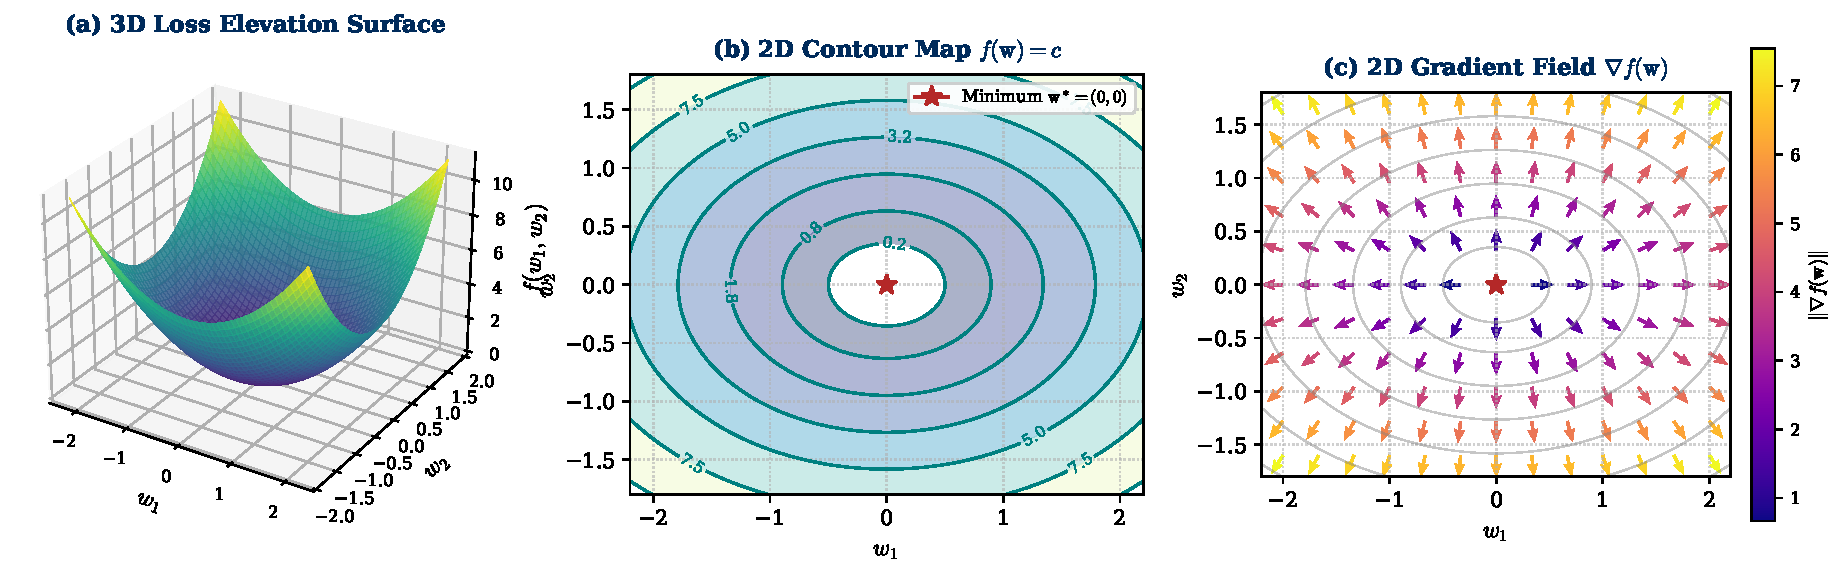
\includegraphics[width=\linewidth]{figures/gd_landscape_3panels.pdf}
\caption{Three synchronized representations of an optimization landscape $f(x, y)$: (Left) 3D surface plot displaying elevation peaks, valleys, and saddle regions; (Middle) 2D contour map showing level curves $f(x, y) = c$, where concentric closed loops enclose local minima or maxima; (Right) 2D vector field of gradients, where vector lengths indicate slope magnitude and arrows point in the direction of steepest ascent.}
\label{fig:gd_landscape_3panels}
\end{figure}

As displayed in Figure~\ref{fig:gd_landscape_3panels}:
\begin{enumerate}
  \item \textbf{3D Surface Plot (Elevation)}: Directly graphs the scalar cost value $z = f(x, y)$ as a function of the two parameters. Elevation reflects loss magnitude; global and local minima correspond to valleys.
  \item \textbf{2D Contour Map (Level Curves)}: Slices the 3D surface horizontally at constant loss elevations $f(x, y) = c$. Concentric closed isocurves enclose local extrema (minima or maxima). Spacing between contour lines indicates steepness: densely packed contours signify precipitous cliffs, whereas widely spaced contours indicate flat plateaus.
  \item \textbf{2D Gradient Vector Field}: Maps every coordinate $(x, y)$ to its gradient vector $\nabla f(x, y) = [\frac{\partial f}{\partial x}, \frac{\partial f}{\partial y}]^\top$. The arrows point in the direction of maximum instantaneous ascent, and their lengths represent the magnitude of the slope $\|\nabla f\|$.
\end{enumerate}

\subsection{Mathematical foundations: Differentiability and level curve orthogonality}
\label{sec:differentiability_and_orthogonality}

Before executing gradient updates, we must formalize two foundational mathematical principles emphasized in the AML curriculum:

\paragraph{The Differentiability Condition: Partial derivatives vs. true differentiability.}
Gradient descent updates require the objective function $f: \R^d \to \R$ to be differentiable. A frequent trap in mathematical analysis and oral examinations is confusing the existence of partial derivatives with true differentiability:
\begin{examinsight}[Oral Exam Pitfall: Differentiability vs. Partial Derivatives]
\textbf{The existence of all partial derivatives (or even all directional derivatives) does NOT imply that a function is differentiable!}\\
A multivariable function $f: \R^d \to \R$ is differentiable at $\mathbf{x}_0$ if and only if there exists a linear map (the gradient $\nabla f(\mathbf{x}_0)$) such that:
\begin{equation}
\lim_{\mathbf{h} \to \mathbf{0}} \frac{f(\mathbf{x}_0 + \mathbf{h}) - f(\mathbf{x}_0) - \nabla f(\mathbf{x}_0)^\top \mathbf{h}}{\|\mathbf{h}\|_2} = 0.
\label{eq:frechet_differentiability}
\end{equation}
By the Total Differential Theorem, a sufficient condition for differentiability is that all partial derivatives exist and are \textbf{continuous} ($f \in C^1$). If partial derivatives exist but are discontinuous, the function may fail to be differentiable, causing gradient descent to fail.
\end{examinsight}

To understand this distinction concretely, consider the classic counterexample:
\begin{equation}
f(x, y) = \begin{cases} 0 & \text{at } (x, y) = (0, 0), \\ \dfrac{x^2 y}{x^2 + y^2} & \text{elsewhere}. \end{cases}
\label{eq:differentiability_counterexample}
\end{equation}

\begin{figure}[H]
\centering
\begin{minipage}{0.48\linewidth}
  \centering
  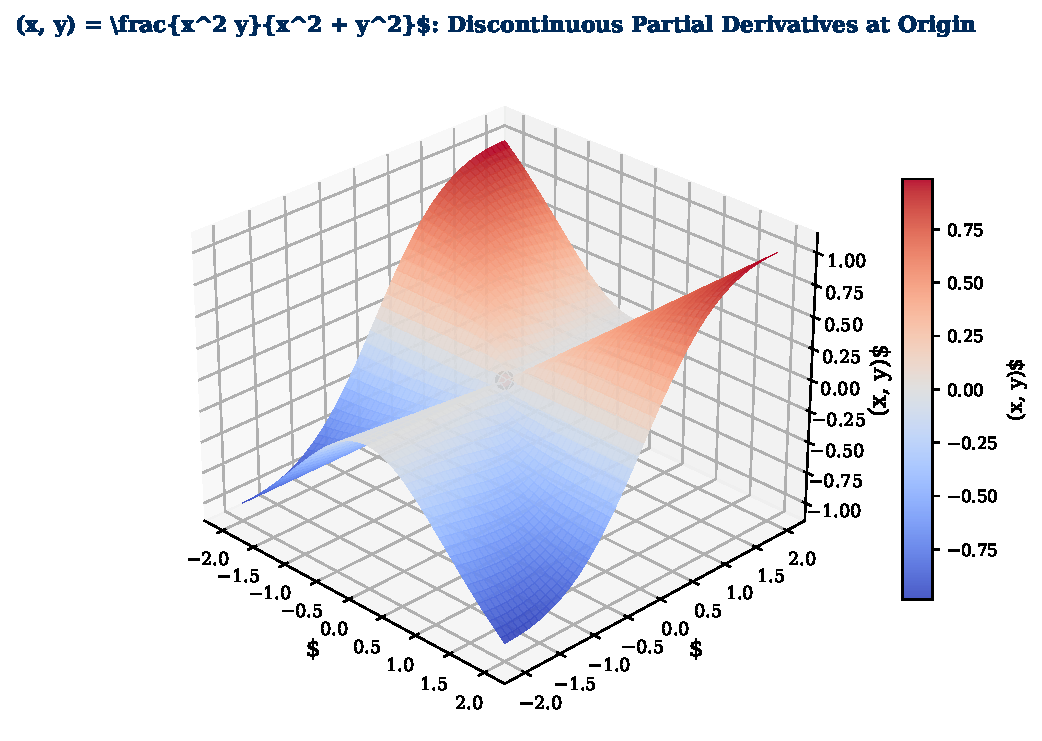
\includegraphics[width=0.95\linewidth]{figures/differentiability_counterexample_3d.pdf}
  \caption{3D surface plot of the counterexample function $f(x, y) = \frac{x^2 y}{x^2 + y^2}$ around the origin. Although partial derivatives exist everywhere, they are discontinuous at $(0, 0)$, rendering the surface non-differentiable.}
  \label{fig:differentiability_counterexample_3d}
\end{minipage}\hfill
\begin{minipage}{0.48\linewidth}
  \centering
  \begin{tikzpicture}[>=Stealth, scale=0.72, every node/.style={transform shape}]
    % Concentric elliptical contours of f(x,y)
    \draw[thick, gray!50] (0,0) ellipse (0.8cm and 0.5cm);
    \node[font=\tiny, gray!70] at (0, 0.6) {$f=0.5$};

    \draw[thick, deepdiveTeal!60] (0,0) ellipse (1.6cm and 1.0cm);
    \node[font=\tiny, deepdiveTeal!80] at (0, 1.15) {$f=1.5$};

    \draw[very thick, politoNavy] (0,0) ellipse (2.6cm and 1.6cm);
    \node[font=\scriptsize\bfseries, politoNavy] at (0, 1.8) {$\mathcal{C}_c: f(\mathbf{w}) = 2.5$};

    \draw[thick, gray!50] (0,0) ellipse (3.6cm and 2.2cm);
    \node[font=\tiny, gray!70] at (0, 2.4) {$f=4.0$};

    \draw[thick, gray!40] (0,0) ellipse (4.6cm and 2.8cm);
    \node[font=\tiny, gray!60] at (0, 3.0) {$f=6.0$};

    % Center minimum
    \fill[examred] (0,0) circle (2.5pt);
    \node[below=2pt, font=\scriptsize\bfseries, text=examred] at (0,0) {$\mathbf{w}^*$};

    % Marked point on level curve
    \coordinate (P) at (1.99, 1.03);
    \fill[politoNavy] (P) circle (3pt);
    \node[below left=2pt, font=\footnotesize\bfseries, text=politoNavy] at (P) {$\mathbf{w}_0$};

    % Tangent space line
    \draw[thick, dashed, gray!80] ($(P) + (1.61, -1.19)$) -- ($(P) + (-2.01, 1.48)$)
      node[above left, font=\scriptsize\bfseries, text=gray!90] {$\mathcal{T}_{\mathbf{w}_0}$};

    % Tangent vector v arrow
    \draw[->, very thick, deepdiveTeal] (P) -- ($(P) + (-1.21, 0.89)$)
      node[above, font=\footnotesize\bfseries, text=deepdiveTeal] {$\mathbf{v}$ ($df = 0$)};

    % Gradient vector: normal to tangent
    \draw[->, line width=1.6pt, examred] (P) -- ($(P) + (1.07, 1.45)$)
      node[above right, font=\footnotesize\bfseries, text=examred, align=left] {$\nabla f(\mathbf{w}_0)$};

    % Downhill negative gradient arrow
    \draw[->, line width=1.6pt, intuitiongreen] (P) -- ($(P) + (-1.07, -1.45)$)
      node[below right, font=\footnotesize\bfseries, text=intuitiongreen, align=left] {$-\nabla f(\mathbf{w}_0)$};

    % Right angle symbol
    \coordinate (RA1) at ($(P) + 0.28*(-0.805, 0.593)$);
    \coordinate (RA2) at ($(P) + 0.28*(-0.805, 0.593) + 0.28*(0.593, 0.805)$);
    \coordinate (RA3) at ($(P) + 0.28*(0.593, 0.805)$);
    \draw[thick, examred] (RA1) -- (RA2) -- (RA3);

    % Theorem callout
    \node[draw=politoNavy!70, fill=white, rounded corners=3pt, inner sep=3pt, font=\tiny, align=left] at (-1.8, -1.9) {
      $\langle \nabla f(\mathbf{w}_0), \mathbf{v} \rangle = 0 \quad \forall \mathbf{v} \in \mathcal{T}_{\mathbf{w}_0}$\\
      $\implies \nabla f \perp \text{Level Curves}$
    };
  \end{tikzpicture}
  \caption{Geometric orthogonality of the gradient to contour level curves. Along the isocurve $f(x, y) = 2.5$, the directional derivative along any tangent vector $\mathbf{v}$ is zero ($\langle \nabla f, \mathbf{v} \rangle = 0$). The negative gradient $-\nabla f$ points strictly perpendicular to the level curve in the direction of steepest descent.}
  \label{fig:gradient_orthogonal_level_curves}
\end{minipage}
\end{figure}

Evaluating the partial derivatives of Equation~\eqref{eq:differentiability_counterexample} at the coordinate origin via the difference quotient:
\begin{align}
\frac{\partial f}{\partial x}(0, 0) &= \lim_{h \to 0} \frac{f(h, 0) - f(0, 0)}{h} = \lim_{h \to 0} \frac{0 - 0}{h} = 0, \\
\frac{\partial f}{\partial y}(0, 0) &= \lim_{h \to 0} \frac{f(0, h) - f(0, 0)}{h} = \lim_{h \to 0} \frac{0 - 0}{h} = 0.
\end{align}
Both partial derivatives exist and equal zero at the origin. However, computing the partial derivative with respect to $y$ along the line $y = 0$ for any $x \ne 0$:
\begin{equation}
\frac{\partial f}{\partial y}(x, 0) = \left. \frac{x^2(x^2 + y^2) - x^2 y(2y)}{(x^2 + y^2)^2} \right|_{y=0} = \frac{x^4}{x^4} = 1.
\end{equation}
Meanwhile, along the $y$-axis ($x = 0$): $\frac{\partial f}{\partial y}(0, y) = 0$. Therefore, $\lim_{(x, y) \to (0, 0)} \frac{\partial f}{\partial y}(x, y)$ does not exist! The partial derivative is \textbf{discontinuous at the origin}, proving that $f(x, y)$ is not differentiable at $(0, 0)$, despite all directional derivatives being well-defined.

\paragraph{Orthogonality of the gradient to level curves.}
A second foundational geometric theorem is that the gradient vector is strictly \textbf{orthogonal} to the contour level curves (or level hypersurfaces in higher dimensions).

Let $\mathcal{C}_c \triangleq \{ \mathbf{w} \in \R^d : f(\mathbf{w}) = c \}$ be an isocurve of constant value $c$. Let $\mathbf{r}(t)$ be an arbitrary smooth path lying entirely within the level set, such that $f(\mathbf{r}(t)) = c$ for all $t$. Differentiating both sides with respect to scalar parameter $t$ via the multivariate chain rule:
\begin{equation}
\frac{d}{dt} f(\mathbf{r}(t)) = \nabla f(\mathbf{r}(t))^\top \mathbf{r}'(t) = 0.
\label{eq:level_curve_orthogonality_proof}
\end{equation}
Here, $\mathbf{r}'(t) \equiv \mathbf{v}$ is the tangent velocity vector along the contour curve. Equation~\eqref{eq:level_curve_orthogonality_proof} proves that:
\begin{equation}
\langle \nabla f(\mathbf{w}), \mathbf{v} \rangle = 0 \quad \text{for any tangent vector } \mathbf{v} \text{ to the isocurve}.
\end{equation}
Because the inner product vanishes, the directional derivative along the isocurve is zero: moving tangentially to a level set produces zero instantaneous change in loss. 

Conversely, the direction perpendicular to the tangent space maximizes the inner product, proving that the gradient vector $\nabla f(\mathbf{w})$ is \textbf{perpendicular to the level curves}, pointing toward steepest ascent, while the negative gradient $-\nabla f(\mathbf{w})$ points perpendicular to the level curves toward steepest descent (as illustrated in Figure~\ref{fig:gradient_orthogonal_level_curves}).

\subsection{Stationary points and initialization sensitivity}
\label{sec:stationary_points_initialization}

A point $\mathbf{x}^* \in \R^d$ where the gradient vanishes identically is defined as a \textbf{stationary point} (or critical point):
\begin{equation}
\nabla f(\mathbf{x}^*) = \mathbf{0}.
\label{eq:stationary_point_def}
\end{equation}
Evaluating the gradient descent update rule at a stationary point reveals an immediate consequence:
\begin{equation}
\mathbf{x}^{(t+1)} = \mathbf{x}^{(t)} - \alpha \nabla f(\mathbf{x}^{(t)}) = \mathbf{x}^{(t)} - \mathbf{0} = \mathbf{x}^{(t)}.
\end{equation}
Standard first-order gradient descent \textbf{gets stuck} at any stationary point, terminating all parameter updates.

However, a fundamental distinction must be drawn:
\begin{equation}
\text{Stationary Point } (\nabla f = \mathbf{0}) \quad \not\implies \quad \text{Local Minimum!}
\end{equation}
A stationary point can be a local minimum, a local maximum, or a saddle point. 

\begin{figure}[H]
\centering
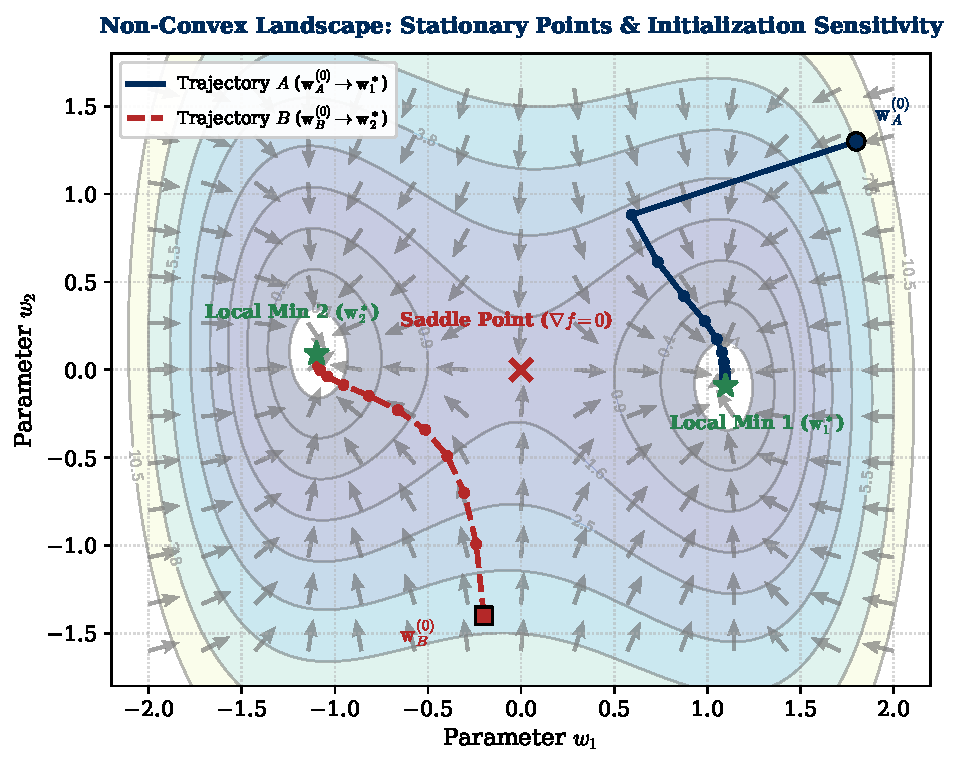
\includegraphics[width=0.55\linewidth]{figures/gd_trajectories_initialization.pdf}
\caption{Optimization trajectories on a non-convex vector field from different parameter initializations. Starting from the upper-right point, gradient updates follow the negative gradient arrows directly into a local minimum basin. Starting from the lower-left point, updates diverge along a completely different path toward a saddle region or alternative basin.}
\label{fig:gd_trajectories_initialization}
\end{figure}

As visualized in Figure~\ref{fig:gd_trajectories_initialization}, which stationary point gradient descent reaches depends entirely on the initial parameter configuration $\mathbf{x}^{(0)}$. In complex non-convex landscapes, different initializations lead to vastly different local basins or saddle geometries.

\subsection{Directional derivative and the proof of steepest descent}
\label{sec:directional_derivative_proof}

To formalize gradient descent from first principles, we analyze how a multivariate function changes along arbitrary spatial trajectories.

Let $f: \R^d \to \R$ be continuously differentiable ($C^1$). Let $\mathbf{u} \in \R^d$ be an arbitrary unit direction vector ($\|\mathbf{u}\|_2 = 1$). The \textbf{directional derivative} of $f$ at point $\mathbf{w}$ along direction $\mathbf{u}$ is defined as the limit:
\begin{equation}
D_\mathbf{u} f(\mathbf{w}) = \lim_{\epsilon \to 0} \frac{f(\mathbf{w} + \epsilon \mathbf{u}) - f(\mathbf{w})}{\epsilon}.
\label{eq:directional_derivative_def}
\end{equation}
By multivariable Taylor theorem, expanding $f(\mathbf{w} + \epsilon \mathbf{u})$ around $\mathbf{w}$:
\begin{equation}
f(\mathbf{w} + \epsilon \mathbf{u}) = f(\mathbf{w}) + \epsilon \nabla f(\mathbf{w})^\top \mathbf{u} + \mathcal{O}(\epsilon^2).
\end{equation}
Substituting this expansion into Equation~\eqref{eq:directional_derivative_def}:
\begin{equation}
D_\mathbf{u} f(\mathbf{w}) = \lim_{\epsilon \to 0} \frac{\epsilon \nabla f(\mathbf{w})^\top \mathbf{u} + \mathcal{O}(\epsilon^2)}{\epsilon} = \nabla f(\mathbf{w})^\top \mathbf{u}.
\label{eq:directional_derivative_inner_product}
\end{equation}
The rate of change along direction $\mathbf{u}$ is given by the inner product of the gradient vector $\nabla f(\mathbf{w})$ with $\mathbf{u}$.

To minimize $f(\mathbf{w})$, we seek the unit direction $\mathbf{u}^*$ that minimizes the directional derivative (i.e., maximizes the rate of instantaneous decrease):
\begin{equation}
\mathbf{u}^* = \arg\min_{\|\mathbf{u}\|_2 = 1} D_\mathbf{u} f(\mathbf{w}) = \arg\min_{\|\mathbf{u}\|_2 = 1} \nabla f(\mathbf{w})^\top \mathbf{u}.
\label{eq:steepest_descent_problem}
\end{equation}
By the Cauchy-Schwarz inequality, for any two vectors $\mathbf{a}, \mathbf{b} \in \R^d$:
\begin{equation}
|\mathbf{a}^\top \mathbf{b}| \le \|\mathbf{a}\|_2 \|\mathbf{b}\|_2 \implies -\sum_{j=1}^d a_j b_j \ge -\|\mathbf{a}\|_2 \|\mathbf{b}\|_2.
\end{equation}
Applying this bound to Equation~\eqref{eq:steepest_descent_problem} with $\mathbf{a} = \nabla f(\mathbf{w})$ and $\mathbf{b} = \mathbf{u}$ (where $\|\mathbf{u}\|_2 = 1$):
\begin{equation}
\nabla f(\mathbf{w})^\top \mathbf{u} \ge -\|\nabla f(\mathbf{w})\|_2 \|\mathbf{u}\|_2 = -\|\nabla f(\mathbf{w})\|_2.
\label{eq:cauchy_schwarz_lower_bound}
\end{equation}
Equality holds if and only if vector $\mathbf{u}$ is collinear with $\nabla f(\mathbf{w})$ and points in the opposite direction:
\begin{equation}
\mathbf{u}^* = -\frac{\nabla f(\mathbf{w})}{\|\nabla f(\mathbf{w})\|_2}.
\label{eq:steepest_descent_direction}
\end{equation}
This rigorous derivation proves Cauchy's 1847 theorem~\cite{cauchy1847methode}: \textbf{the negative gradient direction $-\nabla f(\mathbf{w})$ is the direction of steepest instantaneous descent}.

Geometrically, because $\nabla f(\mathbf{w})$ is strictly perpendicular to the level curves of a continuous surface, stepping along $-\nabla f(\mathbf{w})$ guarantees maximum loss reduction per unit distance moved in high-dimensional spaces.

\subsection{First-order Taylor expansion and the gradient descent update}
\label{sec:first_order_taylor}

We parameterize a finite step of length $\eta > 0$ along direction $\mathbf{u}^*$, yielding displacement $\Delta \mathbf{w} = -\eta \nabla f(\mathbf{w})$. The first-order Taylor series approximation around point $\mathbf{w}_t$ is:
\begin{equation}
f(\mathbf{w}_t - \eta \nabla f(\mathbf{w}_t)) \approx f(\mathbf{w}_t) - \eta \|\nabla f(\mathbf{w}_t)\|_2^2 + \mathcal{O}(\eta^2).
\label{eq:taylor_first_order}
\end{equation}
Because $\|\nabla f(\mathbf{w}_t)\|_2^2 > 0$ for any non-stationary point, there exists a sufficiently small step size $\eta > 0$ such that the second-order remainder is dominated by the linear decrease:
\begin{equation}
f(\mathbf{w}_t - \eta \nabla f(\mathbf{w}_t)) < f(\mathbf{w}_t).
\end{equation}
This establishes the classical \textbf{Gradient Descent update rule}:
\begin{equation}
\mathbf{w}_{t+1} = \mathbf{w}_t - \eta \nabla f(\mathbf{w}_t),
\label{eq:gradient_descent_update}
\end{equation}
where $\eta > 0$ is the \textbf{learning rate} (step size hyperparameter).

\subsection{Learning rate dynamics: Under-stepping vs. divergence}
\label{sec:learning_rate_dynamics}

The magnitude of the learning rate $\eta$ critically dictates optimization stability:

\begin{figure}[H]
\centering
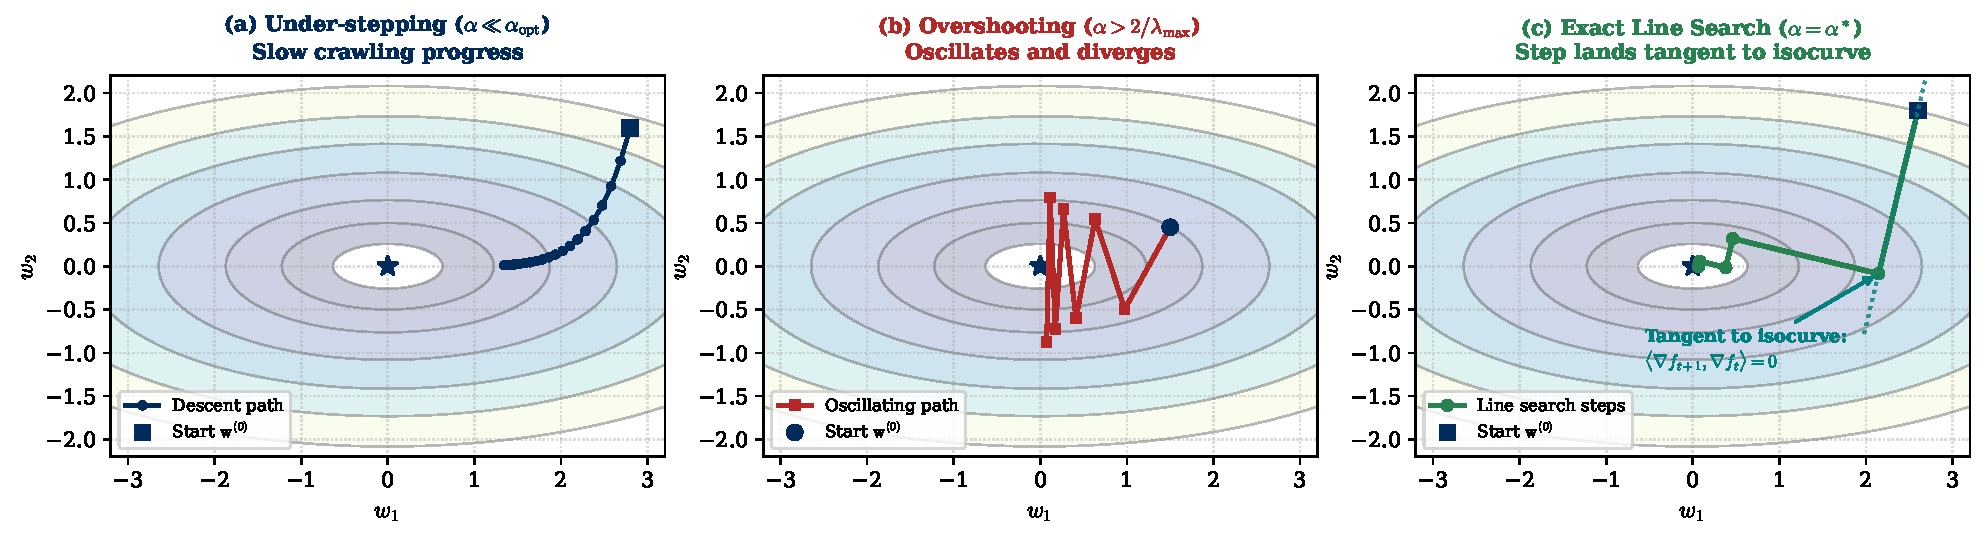
\includegraphics[width=\linewidth]{figures/learning_rate_dynamics_contours.pdf}
\caption{Contour dynamics of gradient descent under varying step sizes $\alpha$: (Left) An excessively small learning rate causes crawling, agonizingly slow progress along the contour gradient; (Middle) An excessively large learning rate overshoots the minimum, oscillating across valley walls with increasing amplitude and ultimately diverging; (Right) An optimal step size determined via line search $\arg\min_\alpha f(\mathbf{x}^{(t)} - \alpha \nabla f(\mathbf{x}^{(t)}))$, where each update lands precisely where the descent direction is tangent to a contour isocurve.}
\label{fig:slide_learning_rates}
\end{figure}

As illustrated across the contour landscapes in Figure~\ref{fig:slide_learning_rates}:
\begin{itemize}
  \item \textbf{Effective Step Length}: An essential mathematical nuance is that the geometric length of the parameter update is not simply the scalar learning rate $\alpha$, but rather the norm-scaled quantity $\alpha \|\nabla f(\mathbf{x}^{(t)})\|$. In regions where the gradient is steep, the parameter displacement is proportionally magnified; conversely, on shallow plateaus where $\|\nabla f\| \approx 0$, progress stalls regardless of $\alpha$.
  \item \textbf{Under-stepping ($\alpha \to 0$)}: When $\alpha$ is excessively conservative, parameter updates $\Delta \mathbf{x}^{(t)}$ are microscopic. Iterations advance imperceptibly, requiring thousands of steps to cross moderate distances and rendering the optimizer vulnerable to premature convergence on deceptive plateaus.
  \item \textbf{Overshooting and Divergence ($\alpha \gg \alpha_{\text{crit}}$)}: When $\alpha$ exceeds the critical threshold dictated by the maximum eigenvalue of the Hessian ($\alpha > 2/\lambda_{\max}$, proven in Section~\ref{sec:condition_number_ravines}), the first-order Taylor approximation breaks down completely. Updates violently oscillate back and forth between opposing valley walls with geometrically increasing amplitude, driving objective values toward infinity: $\lim_{t \to \infty} f(\mathbf{x}^{(t)}) = \infty$.
  \item \textbf{Optimal Step Size via Exact Line Search}: In classical optimization, the optimal step size is determined adaptively by solving a one-dimensional sub-problem along the negative gradient ray:
    \begin{equation}
    \alpha^* = \arg\min_{\alpha > 0} f\left(\mathbf{x}^{(t)} - \alpha \nabla f(\mathbf{x}^{(t)})\right).
    \label{eq:exact_line_search}
    \end{equation}
    Evaluating the optimality condition by differentiating with respect to $\alpha$ via the multivariate chain rule:
    \begin{equation}
    \frac{d}{d\alpha} f\left(\mathbf{x}^{(t)} - \alpha \nabla f(\mathbf{x}^{(t)})\right) = -\nabla f\left(\mathbf{x}^{(t+1)}\right)^\top \nabla f\left(\mathbf{x}^{(t)}\right) = 0.
    \label{eq:line_search_orthogonality}
    \end{equation}
    Equation~\eqref{eq:line_search_orthogonality} reveals a fundamental geometric theorem: at the exact line-search minimizer, the new gradient $\nabla f(\mathbf{x}^{(t+1)})$ is strictly perpendicular to the previous search direction $-\nabla f(\mathbf{x}^{(t)})$. In terms of contour topology, this means the gradient direction at the landing point is \textbf{tangent to the local isocurve} (level set), producing the characteristic orthogonal zig-zag trajectory shown in the right panel of Figure~\ref{fig:slide_learning_rates}.
\end{itemize}

\subsection{Learning rate decay schedules: Linear, inverse, and exponential}
\label{sec:learning_rate_decay_schedules}

Fixing a constant scalar learning rate $\alpha$ forces an undesirable trade-off: a large learning rate enables rapid traversal of distant plateaus early in training but prevents convergence near the minimum due to endless cross-valley oscillations; conversely, a small learning rate ensures stable fine-grained convergence but crawls agonizingly slowly at initialization.

To reconcile these competing objectives, the learning rate can be modulated dynamically over iterations according to a deterministic \textbf{decay schedule} parameterized by a decay factor $\rho > 0$:

\paragraph{Linear decay schedule.}
The linear decay schedule interpolates parameter updates uniformly from an initial step size $\alpha^{(0)}$ down to a designated final floor $\alpha^{(\rho)}$ over a budget of $\rho$ iterations:
\begin{equation}
\alpha^{(t+1)} = \left(1 - \frac{t}{\rho}\right)\alpha^{(0)} + \frac{t}{\rho}\alpha^{(\rho)}, \quad \text{for } 0 \le t \le \rho.
\label{eq:linear_decay_schedule}
\end{equation}
At iteration $t = 0$, $\alpha^{(1)} = \alpha^{(0)}$. At the terminal horizon $t = \rho$, the learning rate contracts precisely to $\alpha^{(\rho)}$ (typically chosen orders of magnitude smaller than $\alpha^{(0)}$). For iterations $t > \rho$, the rate remains fixed at $\alpha^{(\rho)}$. This schedule provides predictable, constant-rate deceleration.

\paragraph{Inverse decay schedule (Time-based decay).}
The inverse decay schedule attenuates the step size inversely with the elapsed iteration count:
\begin{equation}
\alpha^{(t+1)} = \frac{\alpha^{(t)}}{1 + \rho t}.
\label{eq:inverse_decay_schedule}
\end{equation}
In its direct non-recursive formulation, $\alpha^{(t)} = \frac{\alpha^{(0)}}{1 + \rho t}$. This schedule enforces an asymptotic decay rate of $\mathcal{O}(1/t)$, mirroring the classical Robbins-Monro stochastic convergence rate (detailed in Section~\ref{sec:robbins_monro}) while ensuring rapid initial dampening that smoothly transitions into a long-tailed fine-tuning regime.

\paragraph{Exponential decay schedule.}
The exponential decay schedule applies continuous geometric dampening scaled by decay rate $\rho > 0$:
\begin{equation}
\alpha^{(t+1)} = \alpha^{(0)} e^{-\rho t}.
\label{eq:exponential_decay_schedule}
\end{equation}
Because the step size contracts by a constant multiplicative factor $e^{-\rho}$ at every iteration, exponential decay rapidly quenches parameter updates. In contemporary deep learning practice, this is frequently discretized into \emph{step decay} (e.g., decaying $\alpha$ by a factor of $0.1$ or $0.2$ every fixed number of epochs).

Although first-order gradient descent guarantees monotonic cost reduction on smooth surfaces when the step size is sufficiently small, its foundational premise---that the objective function is well-approximated by a flat tangent hyperplane---breaks down on realistic optimization surfaces. When a loss landscape features high anisotropic curvature, such as elongated ravines where the slope across the walls is orders of magnitude steeper than along the floor, gradient descent exhibits pathological cross-valley bouncing and stalls completely. To diagnose and transcend these geometric limitations, we must incorporate second-order curvature information encoded by the Hessian matrix, as developed in Section~\ref{sec:second_order_curvature}.

\section{Second-order curvature, the Hessian matrix, and ill-conditioned ravines}
\label{sec:second_order_curvature}

First-order optimization methods navigate loss landscapes solely on the basis of instantaneous slope, assuming that local descent directions remain reliable over finite distances. However, real-world objective surfaces are curved, undulating, and non-isotropic. The rate at which the gradient itself varies across parameter space---quantified by second-order partial derivatives---critically determines whether an update step successfully descends toward a minimum or violently overshoots into divergence.

The most notorious impediment to first-order optimization is the geometry of \textbf{ill-conditioned ravines}: long, narrow valleys flanked by steep canyon walls and possessing a gently sloping floor. In such landscapes, the curvature across the valley walls dwarfs the curvature along the valley base. Because gradient descent updates are constrained by the maximum curvature to prevent explosive divergence across the walls, parameter updates along the gentle floor crawl at a glacial, near-imperceptible pace. The optimizer spends nearly all its computational effort oscillating perpendicularly between opposing walls rather than advancing toward the true minimizer.

This section develops the mathematical framework of second-order optimization and curvature analysis. We begin by formulating the Hessian matrix and the second-order Taylor expansion, proving how its eigenvalues dictate directional curvature. We then contrast the isotropic quadratic surrogate minimized by first-order gradient descent with the true osculating quadratic model minimized by the Newton-Raphson method, illustrating their distinct step behaviors via native geometric schematics. Finally, we formalize the Hessian condition number $\kappa$, derive the exact upper bound on the stable learning rate $\eta < 2/\lambda_{\max}$, and demonstrate why extreme condition numbers induce catastrophic oscillations in standard gradient descent.

\subsection{The Hessian matrix and second-order Taylor expansion}
\label{sec:hessian_matrix}

Let $f: \R^d \to \R$ be twice continuously differentiable ($C^2$). The second-order Taylor series approximation of $f$ around point $\mathbf{w}$ for an arbitrary displacement $\Delta \mathbf{w} \in \R^d$ is:
\begin{equation}
f(\mathbf{w} + \Delta \mathbf{w}) \approx f(\mathbf{w}) + \nabla f(\mathbf{w})^\top \Delta \mathbf{w} + \frac{1}{2} \Delta \mathbf{w}^\top \mathbf{H}(\mathbf{w}) \Delta \mathbf{w},
\label{eq:second_order_taylor}
\end{equation}
where $\mathbf{H}(\mathbf{w}) \in \R^{d \times d}$ is the \textbf{Hessian matrix} of second-order partial derivatives:
\begin{equation}
\mathbf{H}_{jk}(\mathbf{w}) = \frac{\partial^2 f(\mathbf{w})}{\partial w_j \partial w_k}, \quad j, k \in \{1, \dots, d\}.
\label{eq:hessian_def}
\end{equation}
By Schwarz's theorem on the equality of mixed partials, $\frac{\partial^2 f}{\partial w_j \partial w_k} = \frac{\partial^2 f}{\partial w_k \partial w_j}$, guaranteeing that $\mathbf{H}$ is a real symmetric matrix ($\mathbf{H} = \mathbf{H}^\top$).

By the spectral theorem, the symmetric Hessian admits an orthogonal eigendecomposition:
\begin{equation}
\mathbf{H} = \mathbf{Q} \mathbf{\Lambda} \mathbf{Q}^\top = \sum_{i=1}^d \lambda_i \mathbf{q}_i \mathbf{q}_i^\top,
\label{eq:hessian_spectral}
\end{equation}
where $\mathbf{Q} = [\mathbf{q}_1, \dots, \mathbf{q}_d] \in \R^{d \times d}$ is an orthonormal matrix of eigenvectors ($\mathbf{q}_i^\top \mathbf{q}_j = \delta_{ij}$), and $\mathbf{\Lambda} = \operatorname{diag}(\lambda_1, \dots, \lambda_d)$ contains real eigenvalues ordered such that $\lambda_{\max} \equiv \lambda_1 \ge \lambda_2 \ge \dots \ge \lambda_d \equiv \lambda_{\min}$.

The quadratic term $\frac{1}{2} \Delta \mathbf{w}^\top \mathbf{H} \Delta \mathbf{w}$ characterizes directional curvature:
\begin{itemize}[noitemsep]
  \item If $\Delta \mathbf{w}$ aligns with eigenvector $\mathbf{q}_i$, the second-order change is $\frac{1}{2} \lambda_i \|\Delta \mathbf{w}\|_2^2$.
  \item A positive eigenvalue ($\lambda_i > 0$) signifies positive curvature (the function curves upward like a bowl).
  \item A negative eigenvalue ($\lambda_i < 0$) signifies negative curvature (the function curves downward like a dome).
  \item A zero eigenvalue ($\lambda_i = 0$) signifies flat curvature (the function is locally linear along $\mathbf{q}_i$).
\end{itemize}

\paragraph{Optimal step size under second-order curvature.}
Substituting the gradient descent step $\Delta \mathbf{w} = -\eta \mathbf{g}$ (where $\mathbf{g} = \nabla f(\mathbf{w})$) into Equation~\eqref{eq:second_order_taylor}:
\begin{equation}
f(\mathbf{w} - \eta \mathbf{g}) \approx f(\mathbf{w}) - \eta \mathbf{g}^\top \mathbf{g} + \frac{1}{2} \eta^2 \mathbf{g}^\top \mathbf{H} \mathbf{g}.
\label{eq:gd_step_taylor2}
\end{equation}
To find the step size $\eta^*$ that maximizes expected decrease, we differentiate Equation~\eqref{eq:gd_step_taylor2} with respect to scalar $\eta$ and set the derivative to zero:
\begin{equation}
\frac{d}{d\eta} \left[ f(\mathbf{w}) - \eta \|\mathbf{g}\|_2^2 + \frac{1}{2} \eta^2 \mathbf{g}^\top \mathbf{H} \mathbf{g} \right] = -\|\mathbf{g}\|_2^2 + \eta \mathbf{g}^\top \mathbf{H} \mathbf{g} = 0 \implies \eta^* = \frac{\mathbf{g}^\top \mathbf{g}}{\mathbf{g}^\top \mathbf{H} \mathbf{g}}.
\label{eq:optimal_eta_hessian}
\end{equation}
If the gradient vector happens to align with the dominant eigenvector of the Hessian ($\mathbf{g} \approx \mathbf{q}_1$), the optimal learning rate contracts to $\eta^* = 1/\lambda_{\max}$. Moreover, convergence requires:
\begin{equation}
0 < \eta < \frac{2}{\lambda_{\max}(\mathbf{H})}.
\label{eq:learning_rate_stability_bound}
\end{equation}
If $\eta \ge 2/\lambda_{\max}$, the quadratic term exceeds the linear decrease, and the iterates diverge.

\subsection{Second-order optimization: Newton-Raphson vs. Gradient Descent surrogates}
\label{sec:newton_vs_gd_surrogates}

To comprehend the fundamental divergence between first-order and second-order optimization, we examine the implicit local surrogate models that guide their respective update steps.

At each iteration $\vw$, first-order gradient descent with step size $\eta$ implicitly minimizes a first-order Taylor expansion regularized by an isotropic proximal penalty:
\begin{equation}
\Delta \vw_{\text{GD}} = \argmin_{\Delta \vw} \left[ f(\vw) + \nabla f(\vw)^\top \Delta \vw + \frac{1}{2\eta} \|\Delta \vw\|_2^2 \right] = -\eta \nabla f(\vw).
\label{eq:gd_quadratic_surrogate}
\end{equation}
Geometrically, Equation~\eqref{eq:gd_quadratic_surrogate} models the loss landscape as an \textbf{isotropic spherical bowl} with uniform curvature $1/\eta$ along all spatial directions. The optimizer completely ignores directional variation in terrain steepness, stepping strictly in the direction of steepest instantaneous ascent without regard to whether the slope curves sharply upward or flattens out.

In sharp contrast, the classical multivariate \textbf{Newton-Raphson method} minimizes the \textbf{true osculating second-order Taylor expansion}:
\begin{equation}
q_{\text{Newton}}(\Delta \vw) = f(\vw) + \nabla f(\vw)^\top \Delta \vw + \frac{1}{2} \Delta \vw^\top \mathbf{H}(\vw) \Delta \vw.
\label{eq:newton_taylor_model}
\end{equation}
Assuming the Hessian $\mathbf{H}(\vw)$ is positive definite ($\mathbf{H} \succ 0$), setting the gradient of the surrogate to zero yields:
\begin{equation}
\nabla_{\Delta \vw} q_{\text{Newton}}(\Delta \vw) = \nabla f(\vw) + \mathbf{H}(\vw) \Delta \vw = \mathbf{0} \implies \Delta \vw_{\text{Newton}} = -[\mathbf{H}(\vw)]^{-1} \nabla f(\vw).
\label{eq:newton_step_derivation}
\end{equation}
The Newton-Raphson parameter update is therefore:
\begin{equation}
\vw_{t+1} = \vw_t - [\mathbf{H}(\vw_t)]^{-1} \nabla f(\vw_t).
\label{eq:newton_update_rule}
\end{equation}

\begin{figure}[H]
\centering
\begin{minipage}{0.48\linewidth}
  \centering
  \begin{tikzpicture}[scale=0.82]
    % 1D Surrogate Comparison
    \draw[-{Stealth[length=2mm]}, thick, gray!70] (-0.3, 0) -- (6.0, 0) node[right, font=\scriptsize] {$w$};
    \draw[-{Stealth[length=2mm]}, thick, gray!70] (0, -0.3) -- (0, 4.5) node[above, font=\scriptsize] {Loss};
    \node[font=\bfseries\sffamily, text=politoNavy] at (3.0, 4.3) {(a) 1D Local Quadratic Surrogates};

    % True objective f(w) = 0.2*(x-3.8)^2 + 0.08*(x-3.8)^3 + 0.6
    \draw[very thick, politoNavy, domain=0.4:5.4, samples=80] plot (\x, {0.2*(\x-3.8)^2 + 0.08*(\x-3.8)^3 + 0.6});
    \node[font=\scriptsize\bfseries, text=politoNavy] at (5.2, 1.6) {$f(w)$};

    % Current point w_t at x = 1.2
    \coordinate (wt) at (1.2, {0.2*(1.2-3.8)^2 + 0.08*(1.2-3.8)^3 + 0.6});
    \fill[black] (wt) circle (2.2pt);
    \node[above left=1pt, font=\scriptsize\bfseries] at (wt) {$w_t$};

    % First-order tangent line
    \draw[thick, dashed, gray!60, domain=0.4:3.0] plot (\x, {1.8 + (-0.95)*(\x-1.2)});
    \node[font=\tiny, text=gray!80, rotate=-42] at (2.2, 0.65) {Tangent Plane};

    % GD surrogate (isotropic bowl with scalar step)
    \draw[thick, dashed, examred, domain=0.5:3.2, samples=60] plot (\x, {1.8 - 0.95*(\x-1.2) + 0.9*(\x-1.2)^2});
    \fill[examred] (1.73, 0) circle (1.8pt) node[below, font=\scriptsize\bfseries, text=examred] {$w_{\text{GD}}$};
    \draw[dotted, examred] (1.73, 0) -- (1.73, 1.3);

    % Newton surrogate (exact osculating quadratic)
    \draw[thick, intuitiongreen, domain=0.8:5.2, samples=60] plot (\x, {1.8 - 0.95*(\x-1.2) + 0.18*(\x-1.2)^2});
    \fill[intuitiongreen] (3.84, 0) circle (1.8pt) node[below, font=\scriptsize\bfseries, text=intuitiongreen] {$w_{\text{Newton}}$};
    \draw[dotted, intuitiongreen] (3.84, 0) -- (3.84, 0.55);

    \node[font=\tiny, align=left, text=examred] at (1.1, 3.2) {GD Surrogate $q_{\text{GD}}$\\(Isotropic bowl $\frac{1}{2\eta}(w-w_t)^2$)};
    \node[font=\tiny, align=left, text=intuitiongreen] at (4.5, 3.2) {Newton Surrogate $q_{\text{Newton}}$\\(Osculating $\frac{1}{2}H(w-w_t)^2$)};
  \end{tikzpicture}
\end{minipage}\hfill
\begin{minipage}{0.48\linewidth}
  \centering
  \begin{tikzpicture}[scale=0.82]
    % 2D Step Direction on Anisotropic Contours
    \draw[-{Stealth[length=2mm]}, thick, gray!60] (-3.4, 0) -- (3.6, 0) node[right, font=\scriptsize] {$w_1$ (Gentle base)};
    \draw[-{Stealth[length=2mm]}, thick, gray!60] (0, -2.2) -- (0, 2.4) node[above, font=\scriptsize] {$w_2$ (Steep wall)};
    \node[font=\bfseries\sffamily, text=politoNavy] at (0, 2.6) {(b) Anisotropic Elliptical Contours};

    % Elliptical level curves centered at origin (0, 0)
    \draw[politoNavy!30, thick] (0, 0) ellipse (3.1 and 1.5);
    \draw[politoNavy!50, thick] (0, 0) ellipse (2.3 and 1.05);
    \draw[politoNavy!70, thick] (0, 0) ellipse (1.5 and 0.65);
    \draw[politoNavy!90, thick] (0, 0) ellipse (0.7 and 0.28);

    % Optimum
    \node[star, star points=5, star point ratio=2.2, fill=intuitiongreen, inner sep=1.8pt] at (0, 0) {};
    \node[below left=1pt, font=\scriptsize\bfseries, text=intuitiongreen] at (0, 0) {$\mathbf{w}^*$};

    % Starting point w_0
    \coordinate (w0) at (2.4, 1.15);
    \fill[black] (w0) circle (2.2pt);
    \node[above right, font=\scriptsize\bfseries] at (w0) {$\mathbf{w}_0$};

    % GD Step: perpendicular to level curve (steepest descent)
    \draw[-{Stealth[length=2.5mm]}, very thick, examred] (w0) -- ($(w0) + (-0.6, -1.25)$) 
      node[below right, font=\scriptsize\bfseries, text=examred, align=left] {GD Step $-\eta \nabla f$\\(Orthogonal to contour)};
    \draw[dotted, thick, examred] ($(w0) + (-0.6, -1.25)$) -- ($(w0) + (-1.1, 0.1)$) -- ($(w0) + (-1.5, -0.7)$);

    % Newton Step: directly to minimum!
    \draw[-{Stealth[length=2.5mm]}, very thick, intuitiongreen] (w0) -- (0, 0)
      node[pos=0.45, above right, font=\scriptsize\bfseries, text=intuitiongreen, align=left] {Newton Step $-\mathbf{H}^{-1}\nabla f$\\(Points straight to $\mathbf{w}^*$)};
  \end{tikzpicture}
\end{minipage}
\caption{Geometric comparison between first-order Gradient Descent and second-order Newton-Raphson optimization. (a) In one dimension, gradient descent implicitly constructs an isotropic quadratic surrogate with fixed artificial curvature $1/\eta$, yielding small incremental steps; Newton-Raphson constructs the true osculating quadratic model matching local Hessian curvature, leaping directly to the surrogate minimum. (b) On anisotropic elliptical contours ($\kappa \gg 1$), the negative gradient $-\nabla f$ is strictly perpendicular to level curves, directing updates into steep valley walls and causing oscillatory zig-zags; the inverse Hessian $\mathbf{H}^{-1}$ rescales and rotates coordinates by inverse directional curvatures, guiding the Newton step straight to the global minimizer $\mathbf{w}^*$ in a single leap on quadratic surfaces.}
\label{fig:newton_vs_gd_surrogates}
\end{figure}

\begin{intuition}[Spectral Action of the Inverse Hessian]
To understand how Newton's method eliminates ill-conditioning, express the step in the orthonormal eigenbasis of the Hessian $\mathbf{H} = \mathbf{Q} \mathbf{\Lambda} \mathbf{Q}^\top$. Rotating coordinate displacements to $\Delta \tilde{\vw} = \mathbf{Q}^\top \Delta \vw$ and gradients to $\tilde{\mathbf{g}} = \mathbf{Q}^\top \nabla f(\vw)$:
\begin{equation}
\Delta \tilde{\vw}_{\text{Newton}} = -\mathbf{\Lambda}^{-1} \tilde{\mathbf{g}} = -\begin{bmatrix} \tilde{g}_1 / \lambda_1 \\ \tilde{g}_2 / \lambda_2 \\ \vdots \\ \tilde{g}_d / \lambda_d \end{bmatrix}.
\label{eq:newton_eigenspace_action}
\end{equation}
Equation~\eqref{eq:newton_eigenspace_action} demonstrates the profound auto-adaptive scaling of second-order optimization:
\begin{itemize}[noitemsep]
  \item Along directions of high curvature ($\lambda_i = \lambda_{\max} \gg 0$), the step is aggressively dampened by $1/\lambda_{\max}$, eliminating cross-ravine overshooting.
  \item Along directions of low curvature ($\lambda_i = \lambda_{\min} \approx 0$), the step is massively amplified by $1/\lambda_{\min}$, accelerating rapidly along the flat valley base.
\end{itemize}
If the objective function is purely quadratic, Newton's method reaches the exact minimizer in a \textbf{single step} ($\vw_1 = \vw^*$), rendering convergence speed completely invariant to the condition number $\kappa$!
\end{intuition}

\subsection{The condition number and ill-conditioned ravines}
\label{sec:condition_number_ravines}

A fundamental computational bottleneck for first-order gradient descent is the phenomenon of \textbf{ill-conditioned ravines} (also known as valleys or canyons).

\begin{definition}[Hessian condition number]
For a convex objective with positive definite Hessian ($\mathbf{H} \succ 0$, so all $\lambda_i > 0$), the \textbf{condition number} $\kappa \ge 1$ is defined as the ratio of maximum to minimum eigenvalue:
\begin{equation}
\kappa(\mathbf{H}) = \frac{\lambda_{\max}(\mathbf{H})}{\lambda_{\min}(\mathbf{H})}.
\label{eq:condition_number_def}
\end{equation}
\end{definition}

When $\kappa \approx 1$, the contour lines of the loss surface are isotropic hyperspheres. The gradient vector points directly toward the minimum, and gradient descent converges rapidly.

However, when $\kappa \gg 1$ (e.g., $\kappa = 10^3$ or $10^5$), the problem is termed \textbf{ill-conditioned}. The contour lines form elongated, highly eccentric ellipsoids.

\begin{figure}[H]
\centering
\begin{minipage}{0.48\linewidth}
  \centering
  \begin{tikzpicture}[scale=0.68, every node/.style={transform shape}]
    % Axes
    \draw[-{Stealth}, gray!60, thick] (-3.8, 0) -- (4.0, 0) node[right, font=\footnotesize] {$\mathbf{q}_2$ ($\lambda_{\min}$)};
    \draw[-{Stealth}, gray!60, thick] (0, -2.0) -- (0, 2.0) node[above, font=\footnotesize] {$\mathbf{q}_1$ ($\lambda_{\max}$)};

    % Contours
    \draw[politoNavy!35, thick] (0, 0) ellipse (3.5 and 1.6);
    \draw[politoNavy!55, thick] (0, 0) ellipse (2.7 and 1.15);
    \draw[politoNavy!75, thick] (0, 0) ellipse (1.9 and 0.75);
    \draw[politoNavy!90, thick] (0, 0) ellipse (1.2 and 0.4);
    \draw[politoNavy, thick] (0, 0) ellipse (0.5 and 0.15);

    % Minimizer
    \node[star, star points=5, star point ratio=2.25, fill=intuitiongreen, inner sep=2pt, label={below left:\scriptsize $\mathbf{w}^*$}] at (0, 0) {};

    % Trajectory
    \coordinate (p0) at (3.1, 1.35);
    \coordinate (p1) at (2.8, -1.05);
    \coordinate (p2) at (2.5, 0.82);
    \coordinate (p3) at (2.2, -0.62);
    \coordinate (p4) at (1.9, 0.48);
    \coordinate (p5) at (1.6, -0.35);
    \coordinate (p6) at (1.3, 0.25);

    \draw[-{Stealth}, thick, examred] (p0) -- (p1);
    \draw[-{Stealth}, thick, examred] (p1) -- (p2);
    \draw[-{Stealth}, thick, examred] (p2) -- (p3);
    \draw[-{Stealth}, thick, examred] (p3) -- (p4);
    \draw[-{Stealth}, thick, examred] (p4) -- (p5);
    \draw[-{Stealth}, thick, examred] (p5) -- (p6);

    \foreach \p in {p0,p1,p2,p3,p4,p5,p6} {
      \fill[examred] (\p) circle (1.6pt);
    }
    \node[above right, font=\scriptsize\bfseries, text=examred] at (p0) {$\mathbf{w}_0$};

    \node[font=\scriptsize, text=examred, align=center] at (2.2, -1.6) {Cross-ravine\\oscillations};
    \node[font=\scriptsize, text=deepdiveTeal, align=center] at (-1.8, 1.2) {Slow progress\\along base};
  \end{tikzpicture}
\end{minipage}\hfill
\begin{minipage}{0.48\linewidth}
  \centering
  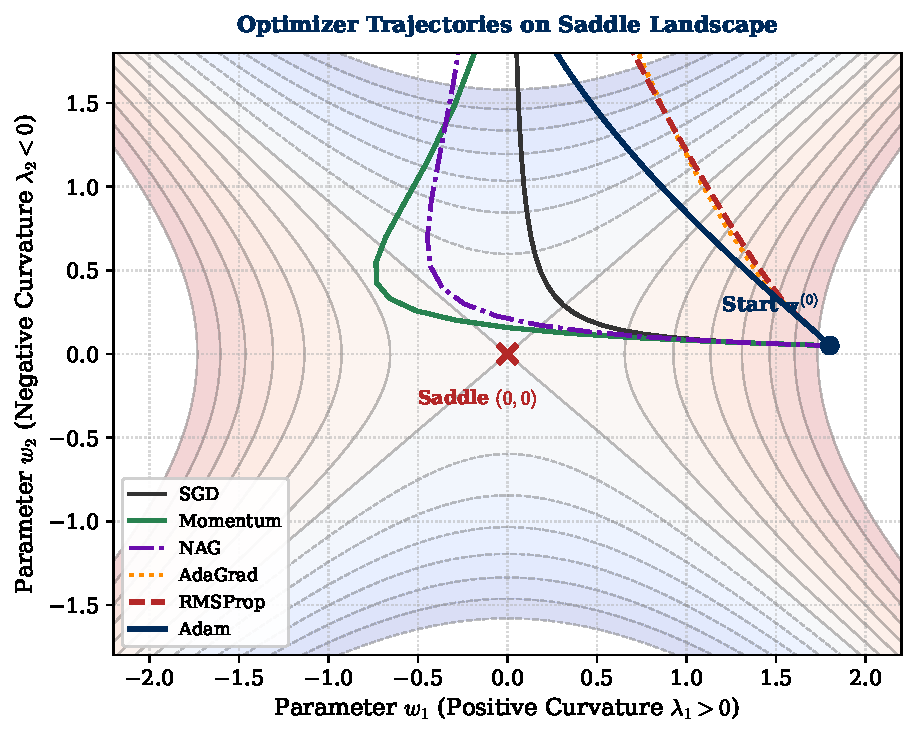
\includegraphics[width=\linewidth]{figures/cs231n_optimizer_comparison.pdf}
\end{minipage}
\caption{Optimization dynamics in ill-conditioned ravines and complex landscapes. Left: Native vector representation of an ill-conditioned quadratic valley ($\kappa = \lambda_{\max}/\lambda_{\min} \gg 1$), where first-order gradient descent oscillates violently across the steep walls along $\mathbf{q}_1$ while making negligible progress along the flat base $\mathbf{q}_2$. Right: Benchmark comparison across optimizers (SGD, Momentum, NAG, AdaGrad, AdaDelta, RMSProp) traversing a saddle topology, demonstrating how momentum and adaptive learning rates overcome anisotropic curvature.}
\label{fig:slide_ill_conditioned_ravine}
\end{figure}

As visualized in Figure~\ref{fig:slide_ill_conditioned_ravine}:
\begin{itemize}
  \item Along the direction of maximum curvature $\mathbf{q}_1$ (across the ravine walls), the loss changes rapidly with eigenvalue $\lambda_{\max}$.
  \item Along the direction of minimum curvature $\mathbf{q}_2$ (along the ravine base leading to the minimum), the loss changes extremely slowly with eigenvalue $\lambda_{\min}$.
  \item The stability bound in Equation~\eqref{eq:learning_rate_stability_bound} restricts the global learning rate to $\eta < 2/\lambda_{\max}$.
  \item Because $\eta$ must be chosen small to prevent explosive divergence across the steep walls, progress along the flat base is scaled by $\eta \lambda_{\min} < 2 \frac{\lambda_{\min}}{\lambda_{\max}} = \frac{2}{\kappa} \ll 1$.
\end{itemize}
Consequently, first-order gradient descent oscillates violently back and forth between the opposing walls of the ravine, making negligible forward progress toward the true minimizer.

While Newton-Raphson optimization elegantly eliminates ill-conditioning by rotating and rescaling the descent trajectory via the inverse Hessian matrix, its practical application to modern neural networks is thwarted by an insurmountable computational barrier. Computing the full $d \times d$ Hessian requires evaluating second-order derivatives across millions to billions of parameters, demanding prohibitive memory storage ($\mathcal{O}(d^2)$) and an impossible cubic inversion cost ($\mathcal{O}(d^3)$ arithmetic operations per step). Machine learning practitioners are thus confronted with a critical imperative: how can an optimizer overcome cross-ravine oscillations and accelerate along the gentle base of ill-conditioned valleys using \textit{only first-order gradient evaluations}? This fundamental question leads directly to Polyak's classical momentum and the lineage of adaptive first-order optimizers developed in Section~\ref{sec:first_order_acceleration_methods}.

\section{First-order acceleration methods: Momentum and unified matrix scaling}
\label{sec:first_order_acceleration_methods}

In high-dimensional non-convex optimization, standard first-order gradient descent behaves like a memoryless physical system: at every iteration, the parameter vector acts as an idealized massless particle that instantly resets its velocity to match the instantaneous negative gradient. While this reactive behavior works satisfactorily on perfectly isotropic quadratic surfaces, it fails catastrophically in the presence of anisotropic curvature and ill-conditioned ravines ($\kappa \gg 1$). In such geometries, the optimizer is buffeted back and forth between opposing valley walls, dissipating nearly all its computational energy in high-frequency cross-valley oscillations while making negligible longitudinal progress toward the minimum.

To overcome this fundamental limitation without incurring the prohibitive $\mathcal{O}(d^3)$ cost of explicit second-order Hessian inversion, statistical learning turns to the principles of classical mechanics. By imbuing the optimizer with \textbf{physical momentum}, the parameter vector is modeled not as a massless point, but as a heavy marble rolling down a frictioned potential well. Historical gradient vectors are accumulated into an internal velocity state, allowing persistent directional forces along the valley floor to build up constructive kinetic energy while high-frequency cross-ravine gradient oscillations cancel each other out destructively.

This section systematically constructs the theory of first-order acceleration methods. We begin with Polyak's classical momentum formulation, detailing its physical velocity accumulation and oscillation-dampening mechanisms. We then derive the exact asymptotic terminal velocity on persistent slopes, proving the celebrated $1/(1-\lambda)$ acceleration factor. Next, we unroll the recursive optimization dynamics to expose standard gradient descent as uniform historical weighting and momentum as an exponentially decayed memory filter. Finally, we formulate the unified diagonal scaling matrix framework $\boldsymbol{\Gamma}_i^t$, revealing how AdaGrad, RMSprop, and Adam adaptively scale step sizes across individual coordinates to conquer disparate curvatures.

\subsection{Classical momentum: Velocity accumulation and oscillation dampening}
\label{sec:classical_momentum}

The classical momentum method, formulated by Boris Polyak in 1964~\cite{polyak1964some}, draws direct inspiration from physical mechanics. Rather than treating the parameter vector as a massless particle whose velocity instantly matches the local negative gradient, the optimizer models a heavy marble rolling down a frictioned potential well.

The algorithm introduces an internal state vector $\mathbf{v}^{(t)} \in \R^d$, termed the \textbf{velocity}, and updates parameters according to the coupled recurrence:
\begin{align}
\mathbf{v}^{(t+1)} &= \lambda \mathbf{v}^{(t)} - \alpha \nabla f(\mathbf{x}^{(t)}), \label{eq:momentum_velocity_update} \\
\mathbf{x}^{(t+1)} &= \mathbf{x}^{(t)} + \mathbf{v}^{(t+1)}, \label{eq:momentum_position_update}
\end{align}
where $\alpha > 0$ is the learning rate, and $\lambda \in [0, 1)$ is the \textbf{momentum coefficient} (or friction parameter, typically set to $\lambda = 0.9$ or $0.99$).

\paragraph{Physical mechanism in ill-conditioned valleys.}
When $\lambda = 0$, the velocity simplifies to $\mathbf{v}^{(t+1)} = -\alpha \nabla f(\mathbf{x}^{(t)})$, collapsing immediately to standard gradient descent. 
When $\lambda > 0$, the velocity retains an exponential moving average of historical gradient directions:
\begin{itemize}[noitemsep]
  \item \textbf{Transverse cross-ravine direction ($\mathbf{q}_1$)}: Because the optimizer repeatedly bounces back and forth across the opposing valley walls, the signs of consecutive partial derivatives alternate: $\nabla f(\mathbf{x}^{(t)})_{\mathbf{q}_1} \approx -\nabla f(\mathbf{x}^{(t-1)})_{\mathbf{q}_1}$. In the velocity accumulator of Equation~\eqref{eq:momentum_velocity_update}, these opposing vectors cancel out destructively:
  \begin{equation}
  \mathbf{v}^{(t+1)}_{\mathbf{q}_1} \approx \lambda \mathbf{v}^{(t)}_{\mathbf{q}_1} - \alpha \nabla f(\mathbf{x}^{(t)})_{\mathbf{q}_1} \approx \mathbf{0}.
  \end{equation}
  This destructive interference aggressively dampens high-frequency cross-ravine oscillations.
  \item \textbf{Longitudinal base direction ($\mathbf{q}_2$)}: Along the gentle descent floor of the valley leading toward the minimizer, consecutive gradients point consistently in the same downhill direction: $\nabla f(\mathbf{x}^{(t)})_{\mathbf{q}_2} \approx \nabla f(\mathbf{x}^{(t-1)})_{\mathbf{q}_2}$. Here, the historical velocity terms add constructively, accumulating directional speed along the base.
\end{itemize}

\subsection{Effective terminal step length and aligned gradient acceleration}
\label{sec:aligned_gradient_acceleration}

A central pedagogical result is quantifying the exact acceleration gain when gradients are persistently aligned.

Suppose the optimizer traverses a uniform slope where the gradient remains constant over consecutive iterations: $\nabla f(\mathbf{x}^{(t)}) \approx \mathbf{g}$. Assuming initial velocity $\mathbf{v}^{(0)} = \mathbf{0}$, unrolling the recurrence in Equation~\eqref{eq:momentum_velocity_update} yields:
\begin{align}
\mathbf{v}^{(1)} &= -\alpha \mathbf{g}, \nonumber \\
\mathbf{v}^{(2)} &= -\lambda \alpha \mathbf{g} - \alpha \mathbf{g} = -\alpha (1 + \lambda) \mathbf{g}, \nonumber \\
\mathbf{v}^{(3)} &= -\lambda \alpha (1 + \lambda) \mathbf{g} - \alpha \mathbf{g} = -\alpha (1 + \lambda + \lambda^2) \mathbf{g}, \nonumber \\
&\;\;\vdots \nonumber \\
\mathbf{v}^{(t+1)} &= -\alpha \mathbf{g} \sum_{k=0}^t \lambda^k.
\label{eq:momentum_geometric_series}
\end{align}
Because $\lambda \in [0, 1)$, the finite summation in Equation~\eqref{eq:momentum_geometric_series} is a geometric progression. Taking the limit as $t \to \infty$:
\begin{equation}
\lim_{t \to \infty} \sum_{k=0}^t \lambda^k = \frac{1}{1 - \lambda}.
\end{equation}
Consequently, the terminal velocity and effective parameter displacement per step converge to:
\begin{equation}
\lim_{t \to \infty} \|\mathbf{v}^{(t+1)}\| = \frac{1}{1 - \lambda} \alpha \|\mathbf{g}\| = \frac{1}{1 - \lambda} \alpha \|\nabla f\|.
\label{eq:terminal_momentum_step}
\end{equation}
Equation~\eqref{eq:terminal_momentum_step} reveals the remarkable speedup factor of momentum:
\begin{itemize}[noitemsep]
  \item For standard gradient descent, the step length along a flat plateau with gradient $\|\nabla f\|$ is strictly $\alpha \|\nabla f\|$.
  \item For momentum with $\lambda = 0.9$, the effective step length expands to $\frac{1}{1 - 0.9}\alpha \|\nabla f\| = \mathbf{10 \alpha \|\nabla f\|}$ ($10\times$ acceleration).
  \item For momentum with $\lambda = 0.99$, the effective step length expands to $\frac{1}{1 - 0.99}\alpha \|\nabla f\| = \mathbf{100 \alpha \|\nabla f\|}$ ($100\times$ acceleration).
\end{itemize}
This dynamic amplification enables momentum to surge rapidly through flat regions and provides the kinetic energy required to carry parameter updates over shallow local barriers into deeper, more generalizing minima basins.

\subsection{Mathematical unrolling: Standard gradient descent vs. momentum}
\label{sec:unrolling_gd_momentum}

To understand how momentum transforms optimization trajectories over an entire training run, we analyze the concept of \textbf{unrolling the optimization recurrence}.

\paragraph{Unrolling standard gradient descent.}
For standard gradient descent without momentum, parameter updates follow $\mathbf{x}^{(t+1)} = \mathbf{x}^{(t)} - \alpha \nabla f(\mathbf{x}^{(t)})$. Unrolling step by step from initialization $\mathbf{x}^{(0)}$:
\begin{align}
\mathbf{x}^{(1)} &= \mathbf{x}^{(0)} - \alpha \nabla f(\mathbf{x}^{(0)}), \nonumber \\
\mathbf{x}^{(2)} &= \mathbf{x}^{(1)} - \alpha \nabla f(\mathbf{x}^{(1)}) = \mathbf{x}^{(0)} - \alpha \nabla f(\mathbf{x}^{(0)}) - \alpha \nabla f(\mathbf{x}^{(1)}), \nonumber \\
&\;\;\vdots \nonumber \\
\mathbf{x}^{(t+1)} &= \mathbf{x}^{(0)} - \alpha \sum_{i=1}^t \nabla f(\mathbf{x}^{(i)}).
\label{eq:unrolled_gd}
\end{align}
Equation~\eqref{eq:unrolled_gd} shows that in standard gradient descent, the net parameter displacement $\mathbf{x}^{(t+1)} - \mathbf{x}^{(0)}$ is simply the unweighted sum of all historical gradients, multiplied by constant step size $-\alpha$. Every historical gradient receives identical weighting, regardless of whether it was computed at the start of training or in the current iteration.

\paragraph{Unrolling gradient descent with momentum.}
Now consider the momentum update defined by Equations~\eqref{eq:momentum_velocity_update}--\eqref{eq:momentum_position_update}. Assuming $\mathbf{v}^{(0)} = \mathbf{0}$, the velocity at any iteration $k \ge 1$ is an exponentially decayed sum of past gradients:
\begin{equation}
\mathbf{v}^{(k)} = -\alpha \sum_{j=1}^k \lambda^{k-j} \nabla f(\mathbf{x}^{(j-1)}).
\end{equation}
Since $\mathbf{x}^{(t+1)} = \mathbf{x}^{(0)} + \sum_{k=1}^{t+1} \mathbf{v}^{(k)}$, the cumulative displacement after $t+1$ steps is:
\begin{equation}
\mathbf{x}^{(t+1)} = \mathbf{x}^{(0)} - \alpha \sum_{k=1}^{t+1} \sum_{j=1}^k \lambda^{k-j} \nabla f(\mathbf{x}^{(j-1)}).
\end{equation}
To determine the net coefficient multiplying each individual gradient $\nabla f(\mathbf{x}^{(i)})$ (for $i = 1, \dots, t$), we observe how often $\nabla f(\mathbf{x}^{(i)})$ enters into subsequent velocity terms:
\begin{itemize}[noitemsep]
  \item At iteration $k = i+1$, $\nabla f(\mathbf{x}^{(i)})$ enters with weight $-\alpha \lambda^0 = -\alpha$.
  \item At iteration $k = i+2$, it persists decayed by $-\alpha \lambda^1$.
  \item At iteration $k = i+3$, it persists decayed by $-\alpha \lambda^2$.
  \item $\dots$
  \item At iteration $k = t+1$, it persists decayed by $-\alpha \lambda^{t-i}$.
\end{itemize}
Summing these contributions across all subsequent steps gives a finite geometric series of length $t - i + 1$:
\begin{equation}
\sum_{m=0}^{t-i} \lambda^m = \frac{1 - \lambda^{t-i+1}}{1 - \lambda} = \frac{1 - \lambda^{t+1-i}}{1 - \lambda}.
\end{equation}
Substituting this closed-form coefficient into the unrolled parameter position yields the exact momentum unrolling formula:
\begin{equation}
\mathbf{x}^{(t+1)} = \mathbf{x}^{(0)} - \alpha \sum_{i=1}^t \left( \frac{1 - \lambda^{t+1-i}}{1 - \lambda} \right) \nabla f(\mathbf{x}^{(i)}).
\label{eq:unrolled_momentum}
\end{equation}
For early gradients where $t - i \gg 0$, $\lambda^{t+1-i} \to 0$, so their cumulative weight saturates at $-\frac{\alpha}{1 - \lambda}$. For very recent gradients ($i \approx t$), the weight is approximately $-\alpha$. This provides a smooth, recency-weighted memory filter over the optimization trajectory.

\subsection{Unified diagonal scaling matrix framework: Unifying AdaGrad, RMSprop, and Adam}
\label{sec:unified_diagonal_scaling}

The unrolled formulations of Equations~\eqref{eq:unrolled_gd} and~\eqref{eq:unrolled_momentum} represent special cases of a far more general algebraic structure. Any first-order optimization method can be expressed in the \textbf{unified unrolled form}:
\begin{equation}
\mathbf{x}^{(t+1)} = \mathbf{x}^{(0)} - \alpha \sum_{i=1}^t \boldsymbol{\Gamma}_i^t \nabla f(\mathbf{x}^{(i)}),
\label{eq:unified_scaling_matrix}
\end{equation}
where $\boldsymbol{\Gamma}_i^t \in \R^{d \times d}$ is a time-varying \textbf{diagonal scaling matrix}:
\begin{equation}
\boldsymbol{\Gamma}_i^t = \operatorname{diag}\left( \gamma_{i, 1}^t, \, \gamma_{i, 2}^t, \, \dots, \, \gamma_{i, d}^t \right).
\end{equation}

This formulation highlights a profound architectural insight behind Equation~\eqref{eq:unified_scaling_matrix}: standard momentum applies a single scalar coefficient to all coordinates simultaneously. However, in complex high-dimensional architectures, different parameters experience drastically different gradient magnitudes and curvatures. The diagonal scaling matrix $\boldsymbol{\Gamma}_i^t$ enables the optimizer to assign coordinate-specific acceleration strengths and adaptive step sizes along each individual coordinate direction.

This unified matrix formulation elegantly subsumes the entire lineage of modern deep learning optimizers:
\begin{enumerate}
  \item \textbf{Standard Gradient Descent}: $\boldsymbol{\Gamma}_i^t = \mathbf{I}$, assigning uniform isotropic scalar weighting across all coordinates.
  \item \textbf{Classical Momentum}: $\boldsymbol{\Gamma}_i^t = \left(\frac{1 - \lambda^{t+1-i}}{1 - \lambda}\right)\mathbf{I}$, assigning identical exponentially accumulated scalar weights to all coordinates.
  \item \textbf{AdaGrad (Adaptive Gradient Algorithm)}~\cite{duchi2011adaptive}: Accumulates historical squared gradients per coordinate: $G_{t, jj} = \sum_{k=1}^t (\nabla f(\mathbf{x}^{(k)}))_j^2$. The scaling entries are set to:
    \begin{equation}
    \gamma_{i, j}^t \propto \frac{1}{\sqrt{G_{t, jj} + \epsilon}}.
    \end{equation}
    Coordinates with historically frequent or steep gradients are dampened, while coordinates with rare or small gradients receive larger relative steps.
  \item \textbf{RMSprop (Root Mean Square Propagation)}~\cite{goodfellow2016deep}: Resolves AdaGrad's premature learning rate collapse by replacing monotonic sum $G_t$ with an exponentially decaying moving average of squared gradients:
    \begin{equation}
    v_{t, j} = \beta v_{t-1, j} + (1 - \beta) (\nabla f(\mathbf{x}^{(t)}))_j^2, \quad \gamma_{i, j}^t \propto \frac{1}{\sqrt{v_{t, j} + \epsilon}}.
    \end{equation}
  \item \textbf{Adam (Adaptive Moment Estimation)}~\cite{kingma2014adam}: Combines both principles simultaneously: it computes first-moment momentum tracking in the numerator (velocity accumulation) and second-moment uncentered variance tracking in the denominator (RMSprop scaling), with bias-correction factors to compensate for zero-initialization. In the unrolled view of Equation~\eqref{eq:unified_scaling_matrix}, Adam corresponds to a fully adaptive diagonal matrix $\boldsymbol{\Gamma}_i^t$ that dynamically re-scales each parameter coordinate based on its individual signal-to-noise ratio.
\end{enumerate}

Although momentum and adaptive diagonal scaling provide powerful mechanisms for traversing ill-conditioned valleys and accelerating through flat regions, they were originally conceived within the paradigm of convex or locally unimodal optimization. Deep neural architectures, however, present a radically more complex challenge: the composition of multi-layer nonlinear transformations shatters convexity completely, creating high-dimensional loss landscapes populated by astronomically many critical points---including local minima, local maxima, and complex saddle surfaces. Furthermore, simply locating an empirical minimum does not ensure predictive success, as different minima exhibit wildly divergent generalization properties on unseen data. To optimize deep models effectively, we must therefore investigate the topology of critical points and the delicate interplay between curvature and generalization, as explored in Section~\ref{sec:critical_points_deep_learning}.

\section{Critical points and optimization in deep learning: Generalization vs. global minima}
\label{sec:critical_points_deep_learning}

In classical convex optimization, the landscape of the objective function is inherently benign: every stationary point where the gradient vanishes is guaranteed to be a global minimum, ensuring that local search trajectories converge to globally optimal parameters regardless of initialization. In deep neural networks, however, permutation symmetries among hidden units and the cascaded nesting of non-linear activations shatter convexity completely. The resulting parameter space is characterized by an intricate, non-convex terrain punctuated by an astronomical proliferation of critical points, flat plateaus, and treacherous ravines.

For decades, the central fear in non-convex optimization was that gradient-based algorithms would become irrevocably trapped in suboptimal, high-loss local minima. However, modern high-dimensional probability and random matrix theory have revolutionized our understanding of deep loss surfaces: in millions of dimensions, the probability that all eigenvalues of the Hessian are simultaneously positive at a high loss elevation decays exponentially to zero. The primary obstacles that impede training are not isolated local minima, but rather high-index saddle points and vast degenerate plateaus. Crucially, the ultimate objective of machine learning is not to achieve the absolute lowest empirical training loss, but to identify parameter configurations that generalize robustly to unseen test distributions.

This section investigates the topology of critical points in deep learning and formalizes the geometry of generalization. We first establish the spectral classification of critical points via Hessian eigenvalues, characterizing local minima, local maxima, and saddle points. We then unpack the modern consensus dispelling the local minima myth through the theoretical insights of Dauphin et al., showing how saddle points proliferate in high dimensions. Next, we analyze the geometry of generalization by contrasting sharp minima with flat minima under distribution shift, demonstrating why wide basins prevent catastrophic generalization gaps. Finally, we establish why iterative first-order optimization remains indispensable even on strictly convex problems due to computational and numerical stability constraints.

\subsection{Classification of critical points via Hessian eigenvalues}
\label{sec:hessian_classification}

At a critical point $\mathbf{w}^*$, the linear Taylor term in Equation~\eqref{eq:second_order_taylor} vanishes, leaving the local behavior entirely governed by the quadratic form $\frac{1}{2} \Delta \mathbf{w}^\top \mathbf{H}(\mathbf{w}^*) \Delta \mathbf{w}$:
\begin{enumerate}
  \item \textbf{Local Minimum}: The Hessian is positive definite ($\mathbf{H} \succ 0$, all $\lambda_i > 0$). Any displacement strictly increases the loss: $f(\mathbf{w}^* + \Delta \mathbf{w}) > f(\mathbf{w}^*)$.
  \item \textbf{Local Maximum}: The Hessian is negative definite ($\mathbf{H} \prec 0$, all $\lambda_i < 0$). Any displacement strictly decreases the loss: $f(\mathbf{w}^* + \Delta \mathbf{w}) < f(\mathbf{w}^*)$.
  \item \textbf{Saddle Point}: The Hessian has mixed eigenvalues ($\exists \lambda_i > 0$ and $\exists \lambda_j < 0$). The function curves upward along eigenvector $\mathbf{q}_i$ and curves downward along eigenvector $\mathbf{q}_j$.
\end{enumerate}

\begin{figure}[H]
\centering
\begin{minipage}{0.48\linewidth}
  \centering
  \begin{tikzpicture}[>=Stealth, scale=0.75, every node/.style={transform shape}]
    % Axes
    \draw[->, thick, gray!80] (-3.2, 0) -- (3.2, 0) node[right, font=\tiny\bfseries, text=politoNavy] {$w_1$ ($\lambda_1 > 0$)};
    \draw[->, thick, gray!80] (0, -2.6) -- (0, 2.6) node[above, font=\tiny\bfseries, text=examred] {$w_2$ ($\lambda_2 < 0$)};

    % Inflow arrows along w1 axis (Stable manifold)
    \draw[->, very thick, politoNavy] (2.8, 0) -- (1.4, 0);
    \draw[->, very thick, politoNavy] (1.4, 0) -- (0.5, 0);
    \draw[->, very thick, politoNavy] (-2.8, 0) -- (-1.4, 0);
    \draw[->, very thick, politoNavy] (-1.4, 0) -- (-0.5, 0);

    % Outflow arrows along w2 axis (Unstable manifold)
    \draw[->, very thick, examred] (0, 0.5) -- (0, 1.4);
    \draw[->, very thick, examred] (0, 1.4) -- (0, 2.4);
    \draw[->, very thick, examred] (0, -0.5) -- (0, -1.4);
    \draw[->, very thick, examred] (0, -1.4) -- (0, -2.4);

    % Hyperbolic streamlines in quadrants
    % Quadrant 1
    \draw[thick, deepdiveTeal, domain=0.45:2.6, samples=50] plot (\x, {0.8/\x});
    \draw[->, thick, deepdiveTeal] (1.2, {0.8/1.2}) -- (1.0, {0.8/1.0});

    \draw[thick, deepdiveTeal, domain=0.8:2.8, samples=50] plot (\x, {2.0/\x});
    \draw[->, thick, deepdiveTeal] (1.8, {2.0/1.8}) -- (1.5, {2.0/1.5});

    % Quadrant 2
    \draw[thick, deepdiveTeal, domain=-2.6:-0.45, samples=50] plot (\x, {-0.8/\x});
    \draw[->, thick, deepdiveTeal] (-1.2, {-0.8/-1.2}) -- (-1.0, {-0.8/-1.0});

    \draw[thick, deepdiveTeal, domain=-2.8:-0.8, samples=50] plot (\x, {-2.0/\x});
    \draw[->, thick, deepdiveTeal] (-1.8, {-2.0/-1.8}) -- (-1.5, {-2.0/-1.5});

    % Quadrant 3
    \draw[thick, deepdiveTeal, domain=-2.6:-0.45, samples=50] plot (\x, {0.8/\x});
    \draw[->, thick, deepdiveTeal] (-1.2, {0.8/-1.2}) -- (-1.0, {0.8/-1.0});

    \draw[thick, deepdiveTeal, domain=-2.8:-0.8, samples=50] plot (\x, {2.0/\x});
    \draw[->, thick, deepdiveTeal] (-1.8, {2.0/-1.8}) -- (-1.5, {2.0/-1.5});

    % Quadrant 4
    \draw[thick, deepdiveTeal, domain=0.45:2.6, samples=50] plot (\x, {-0.8/\x});
    \draw[->, thick, deepdiveTeal] (1.2, {-0.8/1.2}) -- (1.0, {-0.8/1.0});

    \draw[thick, deepdiveTeal, domain=0.8:2.8, samples=50] plot (\x, {-2.0/\x});
    \draw[->, thick, deepdiveTeal] (1.8, {-2.0/1.8}) -- (1.5, {-2.0/1.5});

    % Critical saddle point at origin
    \fill[white] (0,0) circle (3pt);
    \draw[line width=1.3pt, examred] (-0.12, -0.12) -- (0.12, 0.12);
    \draw[line width=1.3pt, examred] (-0.12, 0.12) -- (0.12, -0.12);
    \node[below left=2pt, font=\tiny\bfseries, text=examred] at (0,0) {Saddle $\mathbf{w}^* = \mathbf{0}$};

    % Annotation callout
    \node[draw=politoNavy!70, fill=white, rounded corners=3pt, font=\tiny, align=left, inner sep=3pt] at (2.0, -1.9) {
      $f = w_1^2 - w_2^2$\\
      $\mathbf{H} = \mathrm{diag}(+2, -2)$\\
      Inflow along $w_1$\\
      Outflow along $w_2$
    };
  \end{tikzpicture}
  \caption{Vector field and contour topology around critical points, illustrating how gradients vanish ($\nabla f = \mathbf{0}$) at stationary points and distinguishing a hyperbolic saddle point from a local minimum basin.}
  \label{fig:slide_saddle_point}
\end{minipage}\hfill
\begin{minipage}{0.48\linewidth}
  \centering
  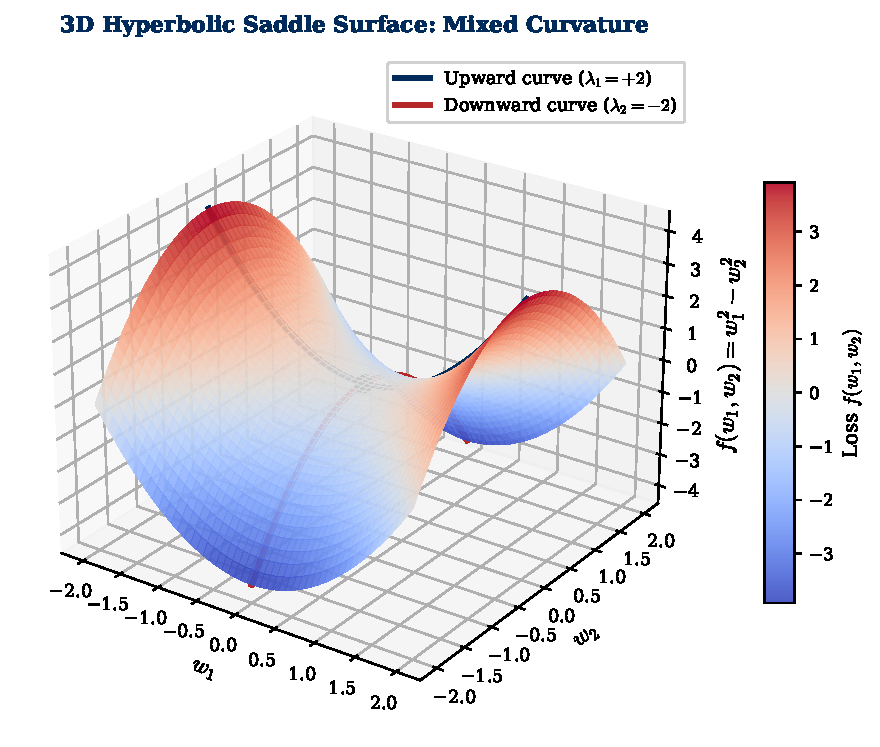
\includegraphics[width=\linewidth]{figures/saddle_point_landscape.pdf}
  \caption{High-resolution 3D visualization of the hyperbolic saddle surface, illustrating mixed eigenvalues $\lambda_1 > 0$ and $\lambda_2 < 0$.}
  \label{fig:manim_saddle_point}
\end{minipage}
\end{figure}

Figures~\ref{fig:slide_saddle_point} and~\ref{fig:manim_saddle_point} illustrate a canonical hyperbolic saddle surface $f(w_1, w_2) = w_1^2 - w_2^2$. At the origin $(0, 0)$, the gradient is zero: $\nabla f = [2w_1, -2w_2]^\top = [0, 0]^\top$. The Hessian matrix is constant:
\begin{equation}
\mathbf{H} = \begin{bmatrix} 2 & 0 \\ 0 & -2 \end{bmatrix},
\end{equation}
yielding eigenvalues $\lambda_1 = +2 > 0$ (along the $w_1$ axis) and $\lambda_2 = -2 < 0$ (along the $w_2$ axis).

\subsection{Proliferation of saddle points in high dimensions (Dauphin et al., 2014)}
\label{sec:dauphin_saddle_points}

In popular machine learning discourse, a persistent misconception is that training deep neural networks fails because first-order gradient descent gets trapped in poor local minima.

In a landmark paper presented at NeurIPS 2014, Dauphin, Bengio et al.~\cite{dauphin2014identifying} disproved this hypothesis using random matrix theory and Bray-Dean statistical physics of high-dimensional non-convex glasses. They established that:
\begin{enumerate}
  \item In a $d$-dimensional parameter space ($d \sim 10^7$ to $10^{11}$ in modern deep learning), the probability that all $d$ random eigenvalues of the Hessian share the same positive sign scales asymptotically as:
  \begin{equation}
  \mathbb{P}(\mathbf{H} \succ 0) \propto \left(\frac{1}{2}\right)^d \approx 0.
  \label{eq:saddle_point_probability}
  \end{equation}
  For $d = 1000$, $(1/2)^{1000} \approx 10^{-301}$, which is physically zero. Therefore, almost all critical points encountered in deep architectures are \textbf{saddle points}, not local minima!
  \item High-loss critical points are overwhelmingly surrounded by directions of negative curvature ($\lambda_i < 0$), providing open escape paths. True local minima exist almost exclusively near the bottom of the loss landscape, where empirical risk is already low and model generalization is strong.
  \item However, because $\|\nabla f(\mathbf{w})\| \approx 0$ in the vicinity of a saddle point, standard first-order gradient descent decelerates dramatically, spending exponential time navigating plateau-like saddle neighborhoods unless escaping noise is injected.
\end{enumerate}

\subsection{Why we are rarely interested in the global optimum}
\label{sec:global_optimum_fallacy}

In modern statistical learning, a foundational insight overturns classical intuition:
\begin{center}
\textbf{\Large\color{politoNavy} ``We are rarely interested in the global optimum!''}
\end{center}

In classical convex optimization, the global minimum is the undisputed goal. In deep learning, however, searching for the absolute global minimum of the empirical risk $\hat{\risk}_N(\mathbf{w})$ is not merely unnecessary—it is actively hazardous:
\begin{enumerate}
  \item \textbf{Overparameterization and Memorization}: Modern deep networks contain vastly more parameters than training samples ($d \gg N$). A network with millions of parameters possesses sufficient capacity to achieve zero empirical loss ($\hat{\risk}_N(\mathbf{w}^*) = 0$) by memorizing every arbitrary training sample, including mislabeled instances and random noise.
  \item \textbf{Generalization Failure}: Reaching the absolute global minimum of empirical loss often drives parameters into extreme overfitted configurations. Because the training set $\mathcal{D}_N$ is merely a finite empirical sample from underlying distribution $P$, perfectly fitting $\mathcal{D}_N$ creates huge errors on unseen test data ($\risk(h_{\mathbf{w}^*}) \gg 0$).
  \item \textbf{Sub-optimal Local Basins Generalize Better}: Any reasonable local minimum that achieves low (but non-zero) loss and resides in a broad, well-behaved basin yields vastly superior generalization compared to the degenerate empirical global optimum.
\end{enumerate}

\subsection{Flat vs. sharp minima: Hessian spectrum and test distribution generalization}
\label{sec:flat_vs_sharp_minima}

To formalize why certain local minima generalize while others overfit, optimization theory examines the \textbf{spectral flatness} of the loss basin (Hochreiter \& Schmidhuber~\cite{hochreiter1997flat}; Keskar et al.~\cite{keskar2017large}):

\begin{figure}[H]
\centering
\resizebox{0.96\linewidth}{!}{%
\begin{tikzpicture}
  % Panel A: Flat vs Sharp Minima under Distribution Shift
  \begin{axis}[
    name=plot1,
    width=8.8cm, height=6.2cm,
    axis lines=left,
    xlabel={Parameter $\mathbf{w}$},
    ylabel={Loss $\mathcal{L}(\mathbf{w})$},
    xmin=0.5, xmax=8.4,
    ymin=0, ymax=3.3,
    ticks=none,
    title={\textbf{(a) Generalization gap under distribution shift}},
    title style={font=\footnotesize, at={(0.5,1.05)}, anchor=south}
  ]
    % Train loss
    \addplot[very thick, politoNavy, domain=1.0:6.5, samples=150] 
      {1.8 + 0.05*(x-4.0)^2 - 1.5*exp(-(x-2.0)^2 / 0.10) - 1.2*exp(-(x-5.2)^2 / 1.5)}
      node[pos=1.0, right, font=\scriptsize\bfseries, text=politoNavy] {Train $\hat{\mathcal{R}}_N$};

    % Test loss (shifted by Delta w = 0.4)
    \addplot[very thick, examred, dashed, domain=1.0:6.5, samples=150] 
      {1.8 + 0.05*(x-0.4-4.0)^2 - 1.5*exp(-(x-0.4-2.0)^2 / 0.10) - 1.2*exp(-(x-0.4-5.2)^2 / 1.5)}
      node[pos=1.0, right, font=\scriptsize\bfseries, text=examred] {Test $\mathcal{R}_{\mathrm{test}}$};

    % Sharp minimum point at x = 2.0
    \draw[dotted, thick, gray!70] (axis cs:2.0, 0) -- (axis cs:2.0, 1.78);
    \fill[politoNavy] (axis cs:2.0, 0.50) circle (2.2pt);
    \fill[examred] (axis cs:2.0, 1.78) circle (2.2pt);
    \node[above left, font=\scriptsize\bfseries, text=politoNavy] at (axis cs:2.0, 0.50) {$\mathbf{w}^*_{\mathrm{sharp}}$};
    
    % Vertical gap at sharp minimum
    \draw[{Stealth[length=4pt]}-{Stealth[length=4pt]}, thick, examred] (axis cs:2.0, 0.56) -- (axis cs:2.0, 1.72);
    \node[right, font=\scriptsize\bfseries, text=examred, align=left] at (axis cs:2.05, 1.15) {Large gap\\(overfitting)};

    % Flat minimum point at x = 5.2
    \draw[dotted, thick, gray!70] (axis cs:5.2, 0) -- (axis cs:5.2, 0.75);
    \fill[politoNavy] (axis cs:5.2, 0.67) circle (2.2pt);
    \fill[examred] (axis cs:5.2, 0.75) circle (2.2pt);
    \node[below, font=\scriptsize\bfseries, text=politoNavy] at (axis cs:5.2, 0.58) {$\mathbf{w}^*_{\mathrm{flat}}$};

    % Small gap at flat minimum
    \draw[{Stealth[length=3pt]}-{Stealth[length=3pt]}, thick, intuitiongreen] (axis cs:5.2, 0.69) -- (axis cs:5.2, 0.73);
    \node[above, font=\scriptsize\bfseries, text=intuitiongreen, align=center] at (axis cs:5.3, 1.20) {Small gap\\(generalizes)};

    % Basin labels
    \node[above, font=\scriptsize\bfseries, text=politoNavy] at (axis cs:2.0, 2.7) {Sharp Minimum};
    \node[above, font=\scriptsize\bfseries, text=politoNavy] at (axis cs:5.2, 2.7) {Flat Basin};
  \end{axis}

  % Panel B: Escaping Sharp Traps via Momentum and Stochastic Noise
  \begin{axis}[
    name=plot2,
    at={($(plot1.east)+(1.8cm, 0)$)},
    anchor=west,
    width=8.8cm, height=6.2cm,
    axis lines=left,
    xlabel={Parameter $\mathbf{w}$},
    ylabel={Loss $\mathcal{L}(\mathbf{w})$},
    xmin=0.5, xmax=8.4,
    ymin=0, ymax=3.3,
    ticks=none,
    title={\textbf{(b) Escaping sharp traps via momentum \& SGD noise}},
    title style={font=\footnotesize, at={(0.5,1.05)}, anchor=south}
  ]
    % Loss landscape
    \addplot[very thick, politoNavy, domain=1.0:6.5, samples=150] 
      {1.8 + 0.05*(x-4.0)^2 - 1.5*exp(-(x-2.0)^2 / 0.10) - 1.2*exp(-(x-5.2)^2 / 1.5)}
      node[pos=1.0, right, font=\scriptsize\bfseries, text=politoNavy] {Loss $f(\mathbf{w})$};

    % Initial point w0
    \coordinate (w0) at (axis cs:1.3, 1.75);
    \shade[ball color=examred] (w0) circle (4pt) node[above left, font=\scriptsize\bfseries, text=examred] {$\mathbf{w}_0$};

    % GD path into sharp trap
    \draw[-{Stealth[length=4pt]}, thick, gray!80, dashed] (w0) to[out=-50, in=170] (axis cs:2.0, 0.52);
    \fill[gray!80] (axis cs:2.0, 0.50) circle (2.5pt);
    \node[above, font=\scriptsize\bfseries, text=gray!80, align=center] at (axis cs:1.6, 0.55) {GD stalls\\in trap};

    % Momentum trajectory flowing along the curve and overcoming barrier
    \draw[-{Stealth[length=5pt]}, very thick, deepdiveTeal] (axis cs:2.0, 0.54) 
      to[out=70, in=185] (axis cs:3.5, 1.68)
      to[out=5, in=170] (axis cs:4.4, 1.15)
      to[out=-10, in=180] (axis cs:5.2, 0.70);
    
    % Ball at the barrier
    \shade[ball color=deepdiveTeal] (axis cs:3.5, 1.70) circle (4pt);
    \node[above, font=\scriptsize\bfseries, text=deepdiveTeal, align=center] at (axis cs:3.5, 2.05) {Velocity $\mathbf{v}$ carries\\over barrier};

    % Ball in flat basin
    \shade[ball color=intuitiongreen] (axis cs:5.2, 0.67) circle (4pt);
    \node[below, font=\scriptsize\bfseries, text=intuitiongreen, align=center] at (axis cs:5.2, 0.55) {Wide Flat Basin\\(generalizes)};

    % Basin labels
    \node[above, font=\scriptsize\bfseries, text=politoNavy] at (axis cs:2.0, 2.7) {Sharp Trap};
    \node[above, font=\scriptsize\bfseries, text=politoNavy] at (axis cs:5.2, 2.7) {Flat Basin};
  \end{axis}
\end{tikzpicture}%
}
\caption{The geometry of generalization in non-convex optimization. (a) Under empirical-to-test distribution shift $\Delta \mathbf{w}$, evaluating a sharp minimum $\mathbf{w}^*_{\mathrm{sharp}}$ (large Hessian eigenvalues $\lambda_i \gg 0$) causes test loss to explode ($\Delta \mathcal{R} \gg 0$), resulting in severe overfitting. Conversely, a flat minimum $\mathbf{w}^*_{\mathrm{flat}}$ (small Hessian eigenvalues $\lambda_i \approx 0$) experiences negligible loss increase, ensuring robust generalization. (b) Standard gradient descent readily gets trapped in narrow, high-loss sharp valleys, whereas momentum velocity $\mathbf{v}$ and stochastic mini-batch noise provide the kinetic energy to escape barriers and settle into wide, flat basins.}
\label{fig:flat_vs_sharp_minima}
\end{figure}

As demonstrated in Figure~\ref{fig:flat_vs_sharp_minima}:
\begin{itemize}
  \item \textbf{Sharp Minima ($\lambda_{\max} \gg 0$)}: Characterized by narrow, steep ravines. Because the empirical training distribution $\hat{P}$ differs slightly from the true underlying distribution $P$, the test loss landscape is shifted horizontally by some small displacement $\Delta \mathbf{w}$. In a sharp well, moving $\mathbf{w}^*_{\text{sharp}} + \Delta \mathbf{w}$ catapults the loss value up the steep canyon wall, causing a catastrophic generalization gap.
  \item \textbf{Flat Minima ($\lambda_{\max} \approx 0$)}: Characterized by wide, gentle valleys. Under the exact same parameter displacement $\Delta \mathbf{w}$, the test loss remains virtually unchanged: $\mathcal{R}_{\text{test}}(\mathbf{w}^*_{\text{flat}} + \Delta \mathbf{w}) \approx \hat{\mathcal{R}}_N(\mathbf{w}^*_{\text{flat}})$. Flat minima are inherently robust to distribution shift and parameter quantization.
  \item \textbf{Kinetic Escape}: While standard batch gradient descent easily gets trapped in steep, non-generalizing local basins, momentum velocity $\mathbf{v}$ and stochastic mini-batch noise $\boldsymbol{\xi}_t$ act as dynamic perturbations that kick parameters over low barriers, naturally filtering out sharp wells in favor of expansive flat basins.
\end{itemize}

\subsection{The imperative for numerical optimization even on convex problems}
\label{sec:convex_problems_numerical_optimization}

This raises an essential theoretical question: \emph{if a machine learning problem is convex and possesses an exact analytical solution, why do we still use iterative gradient descent?}

\begin{enumerate}
  \item \textbf{Computational Complexity and Memory Scaling in OLS}:
    For linear regression, the closed-form normal equations yield $\mathbf{w}^* = (\mathbf{X}^\top \mathbf{X})^{-1}\mathbf{X}^\top \mathbf{y}$. 
    Forming the Gram matrix $\mathbf{X}^\top \mathbf{X}$ requires $\mathcal{O}(N d^2)$ operations, and inverting it via Cholesky or LU decomposition requires $\mathcal{O}(d^3)$ arithmetic operations and $\mathcal{O}(d^2)$ memory storage.
    When $d = 10^5$ (common in text, genomic, or computer vision representations), storing $d \times d$ floating-point matrices requires $40\text{ GB}$ of RAM, and computing $d^3 = 10^{15}$ operations is intractable.
    In contrast, first-order gradient descent scales as $\mathcal{O}(Nd)$ per iteration and requires only $\mathcal{O}(d)$ memory, enabling optimization on commodity hardware.
  \item \textbf{Numerical Stability and Ill-Conditioning}:
    When features are collinear, the condition number $\kappa(\mathbf{X}^\top \mathbf{X}) = (\kappa(\mathbf{X}))^2$ is squared! Direct matrix inversion suffers from catastrophic floating-point cancellation. Iterative gradient descent (especially when regularized via weight decay or early stopping) provides vastly superior numerical stability.
  \item \textbf{Non-Existence of Closed Forms in Generalized Linear Models}:
    As proven in Section~\ref{sec:no_closed_form_solution}, composing linear predictors with non-linear sigmoid or softmax links destroys linear algebra solvability. For logistic regression, closed-form inversion is mathematically impossible, leaving iterative optimization as the sole viable path.
\end{enumerate}

Although first-order gradient descent equipped with momentum and adaptive scaling provides a robust framework for navigating non-convex landscapes toward flat minima, its full-batch formulation suffers from a crushing operational bottleneck in modern data-rich environments: computing the exact gradient requires evaluating forward and backward passes across every single training observation in the dataset. When training sets scale to millions or billions of examples, evaluating a single full-batch parameter update becomes prohibitively sluggish, requiring hours or days of compute. Moreover, deterministic full-batch trajectories lack any exploratory stochasticity to jump over low energetic barriers separating sharp, overfitted wells from wide, generalizing valleys. To unlock efficient learning on massive datasets while harnessing beneficial stochastic perturbation, we must transition from deterministic batch optimization to stochastic gradient descent and mini-batch dynamics in Section~\ref{sec:sgd_and_minibatch}.

\section{Stochastic gradient descent (SGD), mini-batch dynamics, and large-scale learning bounds}
\label{sec:sgd_and_minibatch}

The empirical risk objective in supervised learning is structured as an arithmetic average of loss terms computed across individual training samples. By linearity of differentiation, computing the exact full-batch gradient requires summing the loss gradients evaluated over the entire dataset. In an era where benchmark datasets encompass millions of high-resolution images, billions of web documents, or continuous streaming logs, executing this exhaustive summation for every parameter update creates a paralyzing computational bottleneck that brings optimization to a virtual standstill.

Stochastic gradient descent (SGD) resolves this computational crisis through a profound statistical principle: an average computed over a small, randomly sampled subset of observations serves as an unbiased estimator of the true population expectation. While this subsampling injects high-frequency variance into parameter updates, this stochastic noise is far from a mere nuisance: it acts as a beneficial thermal agitation---an implicit Langevin regularizer that actively prevents parameters from settling into narrow, sharp overfitted minima, nudging the optimization trajectory toward wide, flat basins with superior generalization capabilities.

This section develops the complete theoretical and empirical foundations of stochastic and mini-batch optimization. We begin by dissecting the two computational bottlenecks of full-batch gradient descent (dataset size $n$ and parameter dimension $d$) and evaluate batch vs. stochastic vs. mini-batch estimators through concrete benchmark speedup calculations on MNIST. We then formalize the algorithmic epoch cycle, derive the statistical unbiasedness and $\mathcal{O}(1/m)$ variance reduction of mini-batch gradients, and explain why SGD does not halt at the minimum but fluctuates within a steady-state covariance cloud. Next, we establish the Robbins-Monro conditions governing almost-sure convergence, synthesize the asymptotic learning bounds of Bousquet and Bottou, and contrast all gradient estimation paradigms in an exhaustive comparative matrix. Finally, we conclude with a grand synthesis bridging linear optimization to deep representation learning.

\subsection{The two computational bottlenecks of gradient descent}
\label{sec:two_bottlenecks_gd}

Formally, the empirical risk objective $\hat{\mathcal{R}}_n(\boldsymbol{\theta})$ is defined as the arithmetic mean of loss functions evaluated over $n$ training observations:
\begin{equation}
\ell(\boldsymbol{\theta}) = \frac{1}{n} \sum_{i=1}^n \hat{\ell}_i(\boldsymbol{\theta}), \quad \text{where } \hat{\ell}_i(\boldsymbol{\theta}) \equiv \ell(f_{\boldsymbol{\theta}}(\mathbf{x}_i), y_i).
\label{eq:sum_loss_structure}
\end{equation}
By linearity of differentiation, computing the full batch gradient requires evaluating:
\begin{equation}
\nabla \ell(\boldsymbol{\theta}) = \frac{1}{n} \sum_{i=1}^n \nabla \hat{\ell}_i(\boldsymbol{\theta}).
\label{eq:full_batch_gradient}
\end{equation}

Equation~\eqref{eq:full_batch_gradient} exposes the \textbf{two fundamental bottlenecks} that render full-batch gradient descent impractical for contemporary machine learning:
\begin{enumerate}
  \item \textbf{Bottleneck 1: Number of examples $n$}. In modern datasets (ImageNet, web corpora), $n$ ranges from $10^6$ to $10^{12}$. Evaluating all $n$ forward-backward passes to execute a single parameter step takes hours or days, stalling progress completely.
  \item \textbf{Bottleneck 2: Number of parameters $d$}. Neural networks contain millions to billions of parameters ($d \sim 10^7$--$10^{11}$). Storing, communicating, and computing gradients across $d$ dimensions per sample magnifies computational overhead.
\end{enumerate}

\subsection{Batch vs. stochastic vs. mini-batch estimators and the MNIST speedup}
\label{sec:gradient_estimators_taxonomy}

To break the dataset size bottleneck $n$, we approximate the full summation over training set $\mathcal{T}$ ($|\mathcal{T}| = n$) by evaluating the gradient over a small, representative, uniformly drawn subset $\mathcal{B} \subset \mathcal{T}$ of cardinality $m \ll n$ (termed a \textbf{mini-batch}):
\begin{equation}
\frac{1}{m} \sum_{i \in \mathcal{B}} \nabla \hat{\ell}_i(\boldsymbol{\theta}) \approx \frac{1}{n} \sum_{i \in \mathcal{T}} \nabla \hat{\ell}_i(\boldsymbol{\theta}).
\label{eq:minibatch_approximation}
\end{equation}

\paragraph{A concrete benchmark speedup calculation: MNIST.}
To appreciate the computational advantage concretely, consider the canonical MNIST handwritten digit benchmark:
\begin{itemize}[noitemsep]
  \item Full training set size: $n = 60{,}000$ images.
  \item Mini-batch size: $m = 10$ images.
  \item Speedup factor per gradient update:
  \begin{equation}
  \text{Speedup} = \frac{n}{m} = \frac{60{,}000}{10} = \mathbf{6{,}000 \times \text{ faster per step!}}
  \end{equation}
\end{itemize}
In the time full-batch GD takes to evaluate a single update, mini-batch SGD executes 6,000 parameter updates, making massive progress across the loss terrain.

\subsection{Algorithmic cycle and epoch progression}
\label{sec:algorithmic_cycle_epochs}

The procedural execution of mini-batch stochastic gradient descent proceeds cyclically:
\begin{enumerate}
  \item \textbf{Initialization}: Initialize parameter vector $\boldsymbol{\theta}^{(0)} \in \R^d$ (e.g., via He or Xavier initialization).
  \item \textbf{Mini-Batch Sampling}: Uniformly sample a mini-batch $\mathcal{B} \subset \mathcal{T}$ of size $m$.
  \item \textbf{Downhill Parameter Step}: Update parameters in the negative gradient direction (optionally incorporating momentum velocity):
    \begin{equation}
    \boldsymbol{\theta} \leftarrow \boldsymbol{\theta} - \alpha \nabla \ell_{\boldsymbol{\theta}}(\mathcal{B}).
    \label{eq:minibatch_algorithmic_step}
    \end{equation}
  \item \textbf{Recurrence and Epoch Completion}: Repeat steps 2--3. When accumulated mini-batches exhaustively cover the entire training set $\mathcal{T}$, one \textbf{epoch} is completed. Training iterates across multiple epochs until validation performance plateaus.
\end{enumerate}

\begin{remark}[Constant Update Cost]
A crucial property is that the update cost per iteration is $\mathcal{O}(m \cdot d)$, which is \textbf{strictly constant regardless of the total size of dataset $\mathcal{T}$}. This invariance enables deep learning algorithms to scale gracefully to virtually infinite streaming datasets.
\end{remark}

\subsection{Statistical properties: Unbiasedness, variance scaling, and steady-state oscillations}
\label{sec:minibatch_statistics}

We formalize the statistical properties of the stochastic gradient estimator:

\paragraph{Unbiasedness.}
Let indices in mini-batch $\mathcal{B}$ be drawn uniformly at random without replacement from $\{1, \dots, n\}$. The expected value of the estimator is:
\begin{equation}
\mathbb{E}_{\mathcal{B}}\left[ \frac{1}{m} \sum_{i \in \mathcal{B}} \nabla \hat{\ell}_i(\boldsymbol{\theta}) \right] = \frac{1}{m} \sum_{i \in \mathcal{B}} \mathbb{E}\left[ \nabla \hat{\ell}_i(\boldsymbol{\theta}) \right] = \frac{1}{m} \cdot m \cdot \left( \frac{1}{n} \sum_{k=1}^n \nabla \hat{\ell}_k(\boldsymbol{\theta}) \right) = \nabla \ell(\boldsymbol{\theta}).
\label{eq:unbiased_gradient}
\end{equation}
The mini-batch gradient is an \textbf{unbiased estimator} of the true full-batch gradient.

\paragraph{Variance reduction via batch size $m$.}
Let $\sigma^2 = \frac{1}{n} \sum_{i=1}^n \|\nabla \hat{\ell}_i(\boldsymbol{\theta}) - \nabla \ell(\boldsymbol{\theta})\|_2^2$ denote sample gradient variance. The covariance of the mini-batch estimator satisfies:
\begin{equation}
\mathbb{E}\left[ \left\| \frac{1}{m} \sum_{i \in \mathcal{B}} \nabla \hat{\ell}_i(\boldsymbol{\theta}) - \nabla \ell(\boldsymbol{\theta}) \right\|_2^2 \right] = \frac{\sigma^2}{m} \left( \frac{n - m}{n - 1} \right) \approx \frac{\sigma^2}{m}.
\label{eq:minibatch_variance_reduction}
\end{equation}
Variance contracts as $\mathcal{O}(1/m)$, while computational cost scales as $\mathcal{O}(m)$. Due to the square-root law of diminishing returns ($\operatorname{StdDev} \propto 1/\sqrt{m}$), increasing batch size from $m = 32$ to $1024$ increases compute by $32\times$, but only reduces noise by $\sqrt{32} \approx 5.65\times$. Hence, moderate batch sizes ($32 \le m \le 256$) offer the optimal trade-off between parallel throughput and stochastic exploration.

\begin{figure}[H]
\centering
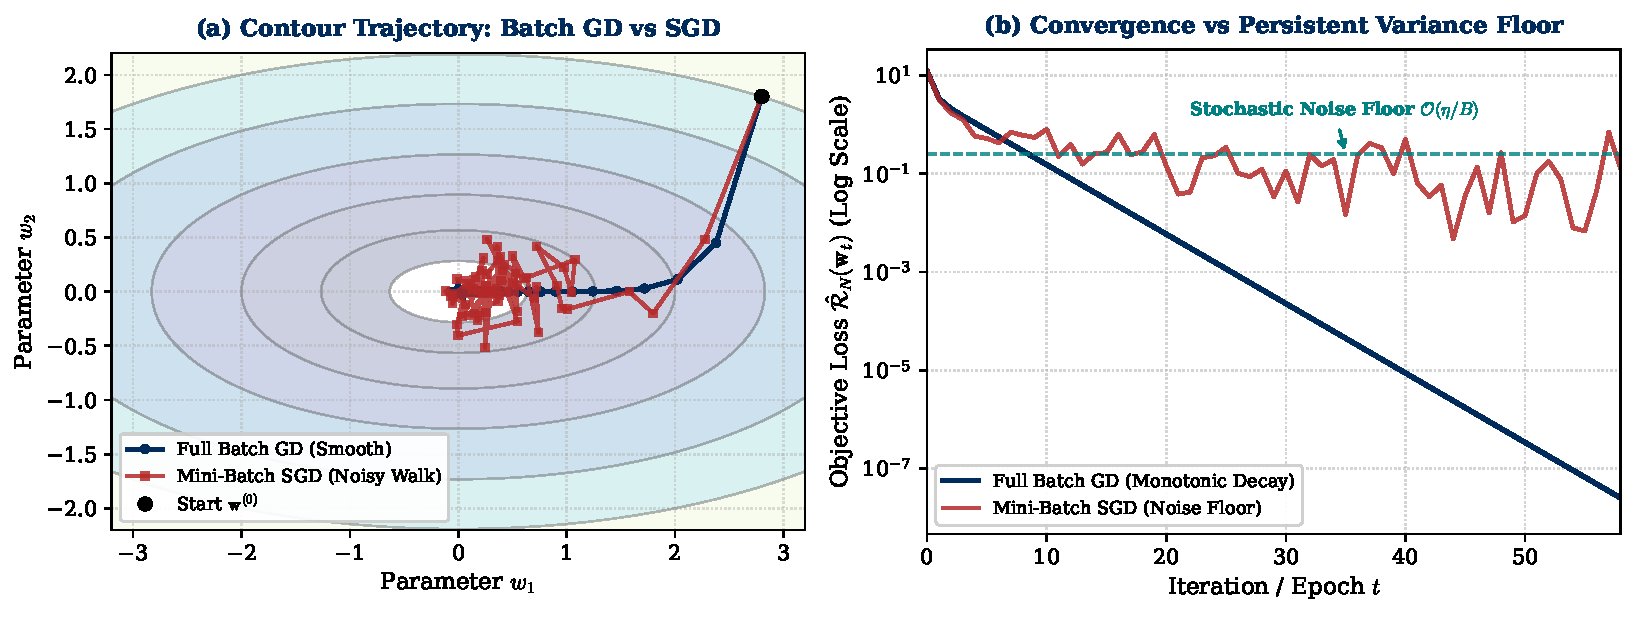
\includegraphics[width=0.95\linewidth]{figures/sgd_oscillations_dynamics.pdf}
\caption{Stochastic gradient descent dynamics: (Left) Contour trajectory showing the noisy Brownian-like walk around the loss minimum without exact stationary convergence; (Right) Parameter weight evolution over epochs on a logarithmic scale, illustrating rapid initial progress followed by persistent steady-state stochastic variance fluctuations induced by random data subsampling.}
\label{fig:slide_minibatch_dynamics}
\end{figure}

\paragraph{Steady-state fluctuations around the minimum.}
As illustrated in Figure~\ref{fig:slide_minibatch_dynamics}, a defining hallmark of SGD is that \textbf{it does not halt at the minimum}:
\begin{equation}
\lim_{t \to \infty} \mathbb{E}\left[ \|\boldsymbol{\theta}_t - \boldsymbol{\theta}^*\|_2^2 \right] \approx \mathcal{O}(\alpha \sigma^2).
\end{equation}
Even when the true gradient vanishes at the minimizer ($\nabla \ell(\boldsymbol{\theta}^*) = \mathbf{0}$), individual sample gradients $\nabla \hat{\ell}_i(\boldsymbol{\theta}^*)$ do not vanish! Consequently, mini-batch gradients retain stochastic noise, causing parameters to wander indefinitely in a steady-state covariance cloud around $\boldsymbol{\theta}^*$.

\subsection{Robbins-Monro convergence conditions for stochastic optimization}
\label{sec:robbins_monro}

To extinguish persistent stochastic oscillations and guarantee almost sure convergence to a stationary point ($\lim_{t \to \infty} \boldsymbol{\theta}_t = \boldsymbol{\theta}^*$), the learning rate sequence $\{\alpha_t\}_{t=1}^\infty$ must be decayed.

In their foundational 1951 paper on stochastic approximation, Herbert Robbins and Sutton Monro~\cite{robbins1951stochastic} established the necessary and sufficient conditions:
\begin{equation}
\sum_{t=1}^\infty \alpha_t = \infty \quad \text{and} \quad \sum_{t=1}^\infty \alpha_t^2 < \infty.
\label{eq:robbins_monro_conditions}
\end{equation}
\begin{itemize}[noitemsep]
  \item \textbf{Condition 1 ($\sum \alpha_t = \infty$)}: Guarantees infinite exploration horizon. The cumulative distance parameters can travel is unbounded, ensuring the optimizer never stalls before reaching the minimum basin.
  \item \textbf{Condition 2 ($\sum \alpha_t^2 < \infty$)}: Guarantees variance extinction. Because cumulative error variance accumulates as $\sum \alpha_t^2 \sigma^2 < \infty$, stochastic fluctuations vanish asymptotically at $\boldsymbol{\theta}^*$.
\end{itemize}

\subsection{Asymptotic upper bounds for large-scale learning (Bottou \& Bousquet, 2008)}
\label{sec:bottou_bousquet_bounds}

The seminal theoretical framework of Léon Bottou and Olivier Bousquet~\cite{bottou2008tradeoffs} (NeurIPS 2008, \emph{``The Tradeoffs of Large Scale Learning''}) rigorously demonstrates why SGD achieves superior generalization compared to full-batch GD under bounded computational budgets.

Consider a convex learning problem with training set size $n$, parameter dimension $d$, and objective condition number $\kappa$. We seek to achieve target accuracy $\rho > 0$ on excess true risk:
\begin{equation}
\left| \ell(h_{\boldsymbol{\theta}}) - \ell(f^*) \right| < \rho,
\label{eq:excess_risk_target}
\end{equation}
where $\ell(h_{\boldsymbol{\theta}})$ is the expected risk of the learned hypothesis, and $\ell(f^*)$ is the Bayes optimal risk.

\begin{table}[H]
\centering
\caption{Asymptotic upper bounds for reaching excess risk $\rho$ on convex problems (Bottou \& Bousquet, NeurIPS 2008). Here $\kappa$ and $\nu$ are constants governing objective conditioning and gradient variance.}
\label{tab:bottou_bousquet_bounds}
\begin{tabularx}{0.92\textwidth}{lXX}
\toprule
\textbf{Optimization Algorithm} & \textbf{Computational Cost per Iteration} & \textbf{Iterations to Reach Target Error $\rho$} \\
\midrule
Full Batch Gradient Descent (GD) & $\mathcal{O}(n \cdot d)$ & $\mathcal{O}\left(\kappa \log \frac{1}{\rho}\right)$ \\
\addlinespace
Stochastic Gradient Descent (SGD) & $\mathcal{O}(d)$ & $\frac{\nu \kappa^2}{\rho} + o\left(\frac{1}{\rho}\right)$ \\
\bottomrule
\end{tabularx}
\end{table}

\paragraph{The profound theoretical implication: Total computational cost.}
Evaluating the total computational work required to reach accuracy $\rho$:
\begin{align}
\text{Total Work}_{\text{GD}} &= \mathcal{O}(nd) \times \mathcal{O}\left(\kappa \log \frac{1}{\rho}\right) = \mathcal{O}\left( n \cdot d \cdot \kappa \log \frac{1}{\rho} \right), \label{eq:total_work_gd} \\
\text{Total Work}_{\text{SGD}} &= \mathcal{O}(d) \times \left( \frac{\nu \kappa^2}{\rho} + o\left(\frac{1}{\rho}\right) \right) = \mathcal{O}\left( \frac{d \cdot \nu \kappa^2}{\rho} \right). \label{eq:total_work_sgd}
\end{align}

\begin{examinsight}[Oral Exam Milestone: Why SGD Generalizes Better]
Observe the fundamental distinction between Equations~\eqref{eq:total_work_gd} and~\eqref{eq:total_work_sgd}:
\begin{center}
\textbf{The total computational cost of SGD does NOT depend on the number of training examples $n$!}
\end{center}
In large-scale machine learning where computation time is limited:
\begin{itemize}[noitemsep]
  \item \textbf{Full Batch GD} spends vast computational resources computing ultra-precise gradients over a fixed, finite dataset $\mathcal{D}_n$, driving empirical training error to zero but over-fitting sample noise.
  \item \textbf{SGD} takes cheap, noisy steps that each touch new, unvisited samples. For a fixed computational budget of floating-point operations (FLOPs), SGD processes orders of magnitude more distinct data samples from distribution $P$.
\end{itemize}
Because statistical generalization error is bounded by the total amount of unique data processed rather than optimization precision on a small set, \textbf{SGD achieves strictly superior generalization error (true risk)}!
\end{examinsight}

\subsection{Practical considerations in modern deep learning SGD}
\label{sec:practical_sgd_deep_learning}

To conclude the optimization framework, we synthesize five foundational practical principles for deploying SGD in contemporary neural networks:

\begin{enumerate}
  \item \textbf{Data Shuffling to Eliminate Ordering Bias}:
    Mini-batches must be drawn by randomly shuffling the dataset at the start of every epoch. If data exhibits sequential correlation (e.g., all class~1 digits grouped together), sequential mini-batches will violently drag parameters toward class~1, causing catastrophic forgetting of preceding classes and inducing cyclic optimization orbits.
  \item \textbf{Hardware Parallelization and SIMD Efficiency}:
    While pure SGD ($m = 1$) is optimal in theory, single-sample operations fail to exploit GPU parallelism. Mini-batch sizes $m \in \{32, 64, 128, 256, 512\}$ are chosen to match GPU Streaming Multiprocessor warp sizes and saturate Tensor Core matrix multiplication units (GEMM).
  \item \textbf{Two-Phase Optimization Dynamics}:
    SGD exhibits an asymmetric temporal profile: \textbf{remarkably rapid initial progress} in early epochs as parameters drop down steep macro-gradients into low-loss valleys, followed by \textbf{slow asymptotic fine-tuning} where parameter wanderings are dominated by gradient variance.
  \item \textbf{Implicit Regularization of Small Mini-Batches}:
    Small mini-batches inject high stochastic gradient noise ($\propto \sigma^2 / m$). This noise acts as an implicit regularizer, preventing parameters from settling into sharp overfitted minima and nudging trajectories into wide flat basins. However, because variance is high, practitioners must reduce the learning rate $\alpha$ (or apply linear learning rate scaling $\alpha \propto m$) to preserve numerical stability.
  \item \textbf{The Practitioner's Fundamental Maxim}:
    This crystallizes the ultimate operational rule of deep learning optimization:
    \begin{center}
    \textbf{\large\color{politoNavy} ``SGD can find a low value of the loss quickly enough to be useful, even if it's not a minimum.''}
    \end{center}
    In real-world engineering, achieving an exact stationary point ($\nabla \ell = \mathbf{0}$) is neither required nor desirable. Finding a robust, flat basin with low empirical loss within practical time constraints delivers state-of-the-art generalization.
\end{enumerate}

\clearpage
\enlargethispage{\baselineskip}
\subsection{Systematic comparison of gradient descent paradigms}
\label{sec:systematic_comparison}

Table~\ref{tab:gradient_comparison} synthesizes the mathematical, computational, and algorithmic trade-offs across the gradient descent family.

\begin{table}[H]
\centering
\small
\renewcommand{\arraystretch}{0.90}
\caption{Systematic comparison of Batch Gradient Descent, Stochastic Gradient Descent (SGD), and Mini-Batch SGD.}
\label{tab:gradient_comparison}
\begin{tabularx}{\textwidth}{lXXX}
\toprule
\textbf{Property} & \textbf{Batch Gradient Descent} & \textbf{Stochastic GD (SGD)} & \textbf{Mini-Batch SGD} \\

\midrule
\textbf{Batch Size $B$} & $B = n$ (full dataset) & $B = 1$ (single sample) & $1 < B < n$ (typically $32$--$512$) \\
\textbf{Cost per Step} & $\mathcal{O}(n \cdot d)$ & $\mathcal{O}(d)$ & $\mathcal{O}(B \cdot d)$ \\
\textbf{Gradient Variance} & Zero (deterministic) & High ($\sigma^2$) & Controlled ($\sigma^2 / B$) \\
\textbf{Convergence Path} & Monotonic \& smooth & Erratic \& oscillatory & Controlled variance cloud \\
\textbf{Hardware Affinity} & Memory bound on large $n$ & Poor GPU SIMD usage & Highly optimized for GPU BLAS \\
\textbf{Saddle Point Escape} & Vulnerable to stall & High escape ability & Strong escape via noise \\
\textbf{Scaling with $n$} & Total work scales with $n$ & Total work independent of $n$ & Total work independent of $n$ \\
\textbf{Generalization} & Prone to sharp traps & Excellent (flat basins) & Optimal (balanced noise) \\
\bottomrule
\end{tabularx}
\end{table}

\subsection{Chapter synthesis and roadmap to representation learning}
\label{sec:chapter3_synthesis}

Across Chapters~1 through~3, we have traversed the foundational triad of statistical machine learning:
\begin{enumerate}[noitemsep,topsep=2pt,parsep=0pt,partopsep=0pt]
  \item \textbf{Statistical foundations (Chapter~1)}: Defining learning paradigms, hypothesis spaces, and the fundamental trade-off between empirical risk and true risk.
  \item \textbf{Decision-theoretic limits (Chapter~2)}: Formulating the Bayes optimal predictor, irreducible noise, and the estimation/approximation trade-off governing model capacity.
  \item \textbf{Loss geometry and optimization (Chapter~3)}: Moving from the non-convex pathologies of squared error in classification to cross-entropy, and replacing intractable analytical matrix inversions with first-order iterative methods (GD, Momentum, and Mini-batch SGD).
\end{enumerate}

The decisive realization uniting this theoretical arc is that \textbf{optimization in machine learning is subservient to generalization}. Unlike classical numerical analysis, where reaching an exact critical point ($\nabla \ell = \mathbf{0}$) is paramount, deep learning exploits stochastic gradient noise, momentum dynamics, and early stopping as implicit regularizers that bias trajectories away from sharp overfitted traps and toward wide, flat basins with superior test performance.

However, all models examined thus far have relied on \textbf{fixed linear representations} $\mathbf{w}^\top \mathbf{x} + b$. Even when paired with cross-entropy and trained via mini-batch SGD, a linear hyperplane cannot separate nonlinearly distributed data (such as the classical XOR problem or complex perceptual manifolds). To transcend this expressivity bottleneck, machine learning diverges into two great paradigms:
\begin{itemize}[noitemsep,topsep=2pt,parsep=0pt,partopsep=0pt]
  \item \textbf{Implicit feature spaces (Kernel Methods and SVMs)}: Projecting inputs into high- (or infinite-) dimensional Hilbert spaces via the kernel trick while retaining convex dual optimization.
  \item \textbf{Explicit hierarchical representations (Deep Neural Networks)}: Learning parameterized feature transformations end-to-end via composite nonlinear layers, where optimization gradients are propagated through intermediate representations using the chain rule (Backpropagation).
\end{itemize}
These representation learning paradigms form the core of the upcoming chapters.


